\chapter{Systematic Uncertainties and Cross Checks}
\label{sec:systematics}
%Follow the analysis note
The measured \bsmumu effective lifetime presented in Chapter~\ref{} is influenced by various systematic biases arising from different areas of the analysis procedure. In this Chapter the size of systematic biases is estimated and several cross checks are made on the measurement strategy to ensure the uncertainties quoted on the final results are correct. The total systematic uncertainties for measuring \tmumu and \Gmumu are give at the end of the Chapter.

All the work presented in this Chapter was completed for this Thesis.

\section{Fit Accuracy}
\label{sec:fitaccuracy}
The fit strategy used to measure the \bsmumu effective lifetime was presented in Chapter~\ref{sec:lifetimemeasurement}, the final fit configuration was chosen by optimising two different types of figures of merit;the mean and width of the pull distributions of free parameters in the fit and the expected uncertainties on \tmumu and \Gmumu. The values for these parameters for 10,000 toy studies using the final fit configuration and assuming the Standard Model \bsmumu branching fraction and effective lifetime are given in Table~\ref{tab:tabA}. The same toy set up as described in Section ~\ref{sec:toys} but in these toy studies only \bsmumu and combinatorial background decays are generated. 
\begin{table}[h]
\begin{center}
\begin{tabular}{cccccccc}
\hline
\multicolumn{2}{c}{$\mathcal{N}$(\bsmumu)} & \multicolumn{2}{c}{$\mathcal{N}$(Comb.)} & \multicolumn{2}{c}{$\lambda$} &  \multicolumn{2}{c}{\Gmumu} \\ \hline
Mean & Width & Mean & Width & Mean & Width &  Mean & Width & $\sigma$/\ps$^{-1}$\\ \hline
-0.097 & 1.020 & -0.062 & 1.030 & -0.013 & 0.992 & -0.000 & 0.993 \\
\hline
\end{tabular}
\vspace{0.7cm}                                                                                                                                               
\caption{Results from toy studies using the final fit configuration for the expected number of decays and assuming the Standard Model value to \tmumu. The mean and width of the pull distributions for the \bsmumu and combinatorial background yields and the slope of the combinatorial background mass \pdf, $\lambda$, are shown along with the median statistical uncertainty on \tmumu and \Gmumu. The uncertainties on the means are 0.010 and widths are 0.007 for all configurations.}
\label{tab:tabA}
\end{center}
\vspace{-1.0cm}                                                                                                                                               
\end{table}
Based on these results several aspects of the fit deserve further investigation, this includes the stability of the fit with different \tmumu values, the biased pull distribution for \bsmumu yields and the overall bias in the measured values of \tmumu and \Gmumu. The biased pull distributions for \tmumu were discussed in Section~\ref{sec:tauORinvtau}.

\subsection{Input lifetimes for toy studies}
The value of \Gmumu is accurately returned by the fit for the expected number of decays. However, it is necessary to understand if this is due to accurate background subtraction by the sPlot method or it it could be resulting from similarities between the decay time distributions of \bsmumu and combinatorial background decays. As a test, toy studies were performed for a range of generated \bsmumu lifetimes different to the Standard Model prediction. Only \bsmumu and combinatorial background decays were generated in the toy studies so that the small contamination from mis-identified backgrounds does not mask the effects of using different lifetimes. The results of 10,000 toy studies are shown in Table~\ref{tab:tabB} and the different lifetimes all return accurate pull distributions for the fitted \Gmumu values with means and widths consistent with 0 and 1, respectively. Therefore the fit returns an accurate measured value for a range of \bsmumu lifetimes.
\begin{table}[htp]
\begin{center}
\begin{tabular}{lcccccccc}
\hline
$\tau$ & \multicolumn{2}{c}{$\mathcal{N}$(\bsmumu)} & \multicolumn{2}{c}{$\mathcal{N}$(Comb.)} & \multicolumn{2}{c}{$\lambda$}  & \multicolumn{2}{c}{\Gmumu} \\ \hline
& Mean & Width & Mean & Width & Mean & Width & Mean & Width \\ \hline
 \tL & -0.098 & 1.019 & -0.062 & 1.018 & -0.003 & 0.987 & -0.010 & 1.018\\
$\tau_{B^{0}_{s}}$ & -0.102 & 1.017 & -0.059 & 1.032 & -0.027 & 0.996 & 0.001 & 0.989 \\
\hline
\end{tabular}
\vspace{0.7cm}                                                                                                                                               
\caption{Results from toy studies using the final fit configuration for the expected number of decays and using the lifetimes of the light \bs mass eigenstate and the mean \bs lifetime. The mean and width of the pull distributions for the \bsmumu and combinatorial background yields and the slope of the combinatorial background mass \pdf, $\lambda$, are shown along with the median statistical uncertainty on \tmumu and \Gmumu. The uncertainties on the means are 0.010 and widths are 0.007 for all configurations.}
\label{tab:tabB}
\end{center}
\vspace{-1.0cm}                                                                                                                                               
\end{table}

\subsection{\bsmumu yields}
The pull distributions for the \bsmumu yields in the mass fit have biased mean values of $\sim$ 0.010 \ps as shown in Tables~\ref{tab:tabA} and~\ref{tab:tabB}, implying that the mass fit does not accurately estimate the \bsmumu yield. However the pull distribution for \Gmumu is accurate therefore this bias in the \bsmumu yield could originate from a different source.

In the toy studies the number of expected decays, $N_{expt}$, in the mass range 4900 - 6000 \mevcc are given in Table~\ref{tab:expectedevents}. These numbers are used as the basis for the toy studies however the number of decays generated is fluctuated for each study about the expected value using a Poisson distribution, therefore the number of decays generated, $N_{gen}$, is different to the expected number.. This enables an extended maximum likelihood fit, where the total number of event is a free parameter, to be used to fit the mass distribution. To achieve an accurate pull distribution of the measured \bsmumu yields from the mass fit the uncertainties on the measured yields must be distributed according to a Gaussian function. This will be true in the high statistics limit where a Poisson distribution is a good approximation of a Gaussian distribution. However the current data available does not contain high statistics for \bsmumu decays therefore the uncertainty on the measured yields is proportional to $\sqrt{N_{gen}}$ and does not have a Gaussian distribution. This effect would shift the mean value of the pull distribution but not lead to an incorrect estimation of the \bsmumu yield. The `fractional bias', $N_{meas} - N_{gen}/N_{gen}$, where $N_{meas}$ is the measured \bsmumu yield is shown in Figure~\ref{} and supports this explanation by producing a mean consistent at zero, with a bias of 0.8 $\%$. 

\begin{figure}[htbp]
    \centering
        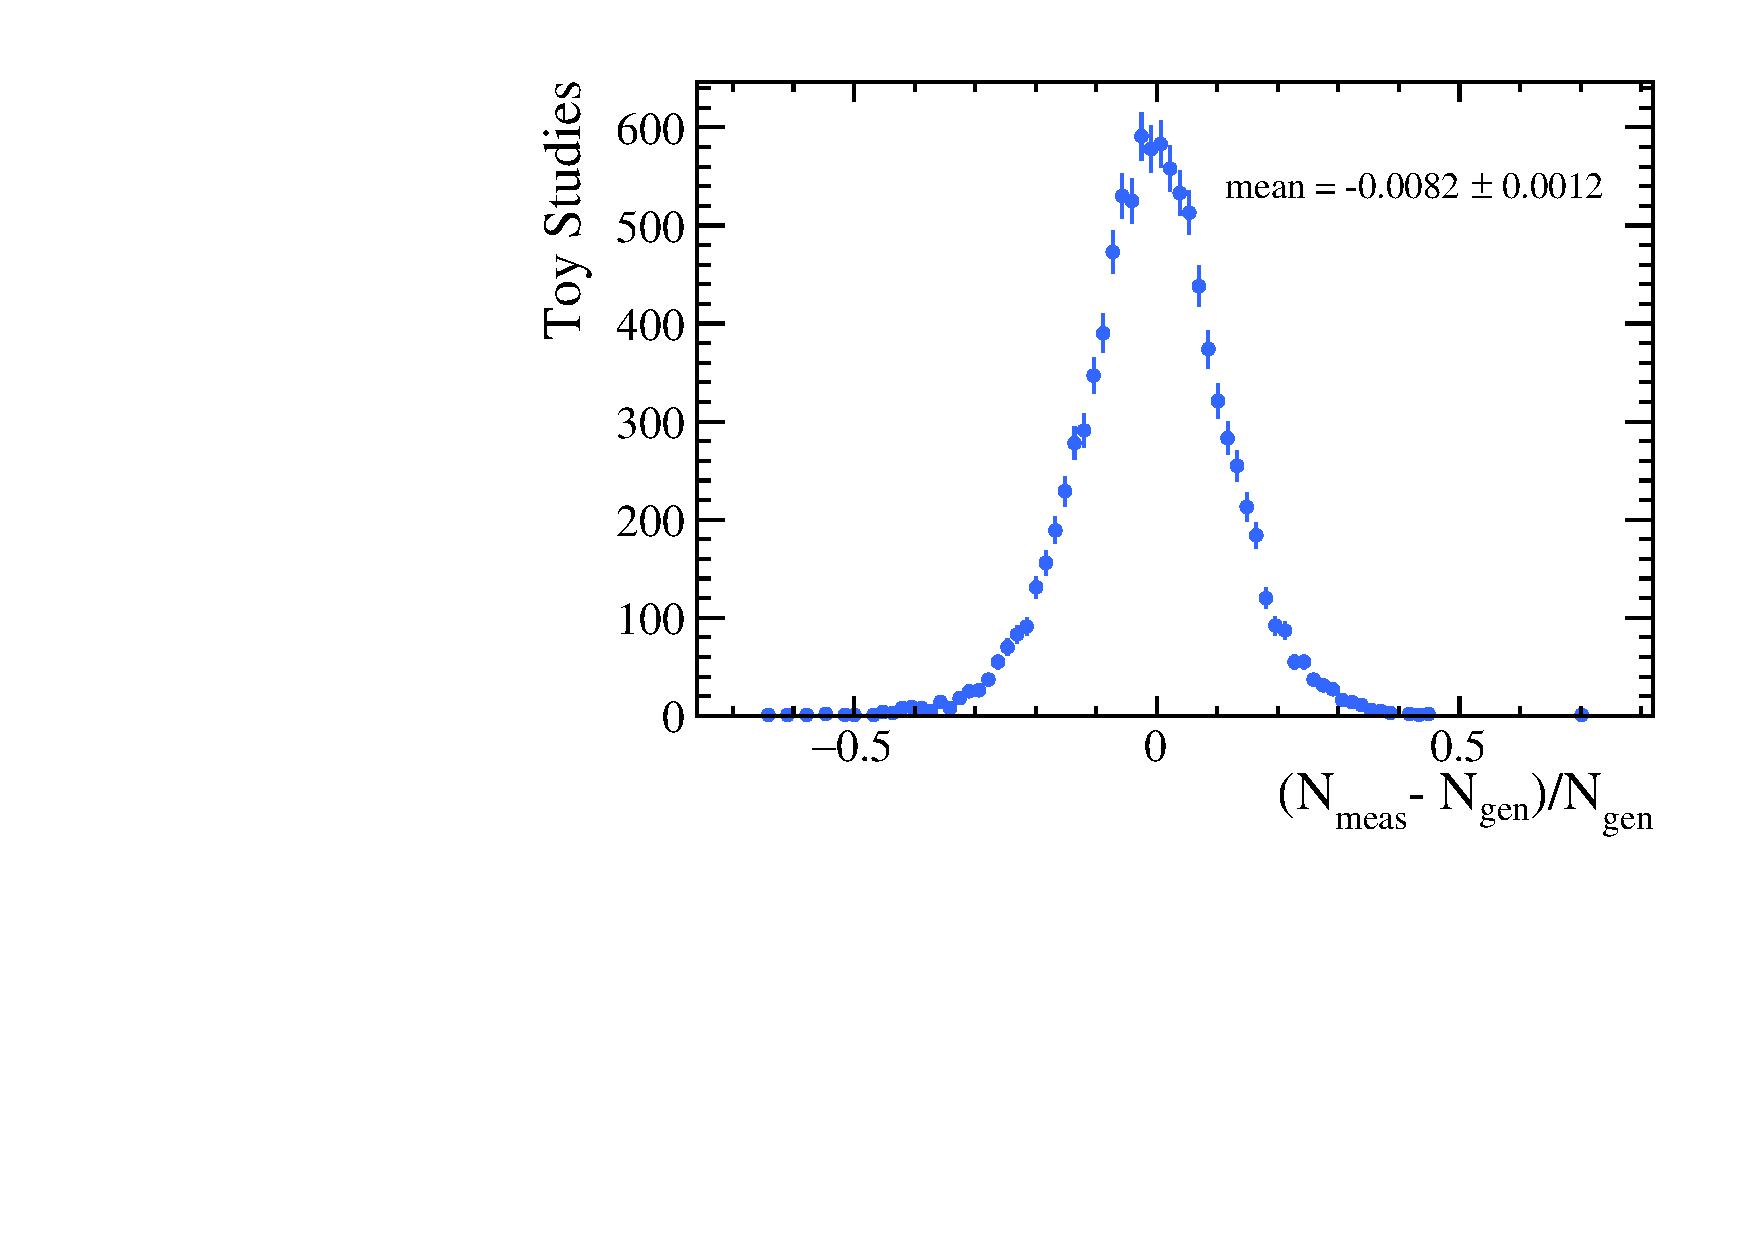
\includegraphics[width=0.6 \textwidth]{./Figs/LifetimeSystematics/Bs2MuMu_yield_fraction_bias_CKM16.pdf}
    \caption{Fractional bias of the measured \bsmumu yield from toy studies for 4.4 \fb.}
    \label{fig:FracBias}
\end{figure}


Furthermore, the pull distributions for \bsmumu yields for toy studies with higher statistics have means that move towards 0 as shown in Figure~\ref{fig:BsmumuYieldPulls} for 50 and 300 \fb. Therefore the mass fit returns accurate yields for \bsmumu and the biased pull distribution arises from the low statistics of the data set. The same reasoning can be applied to the pull distribution of the yields of combinatorial background decays that have a sightly less bias mean value of 0.007 compared to the \bsmumu yields.

\begin{figure}[htbp]
    \centering
        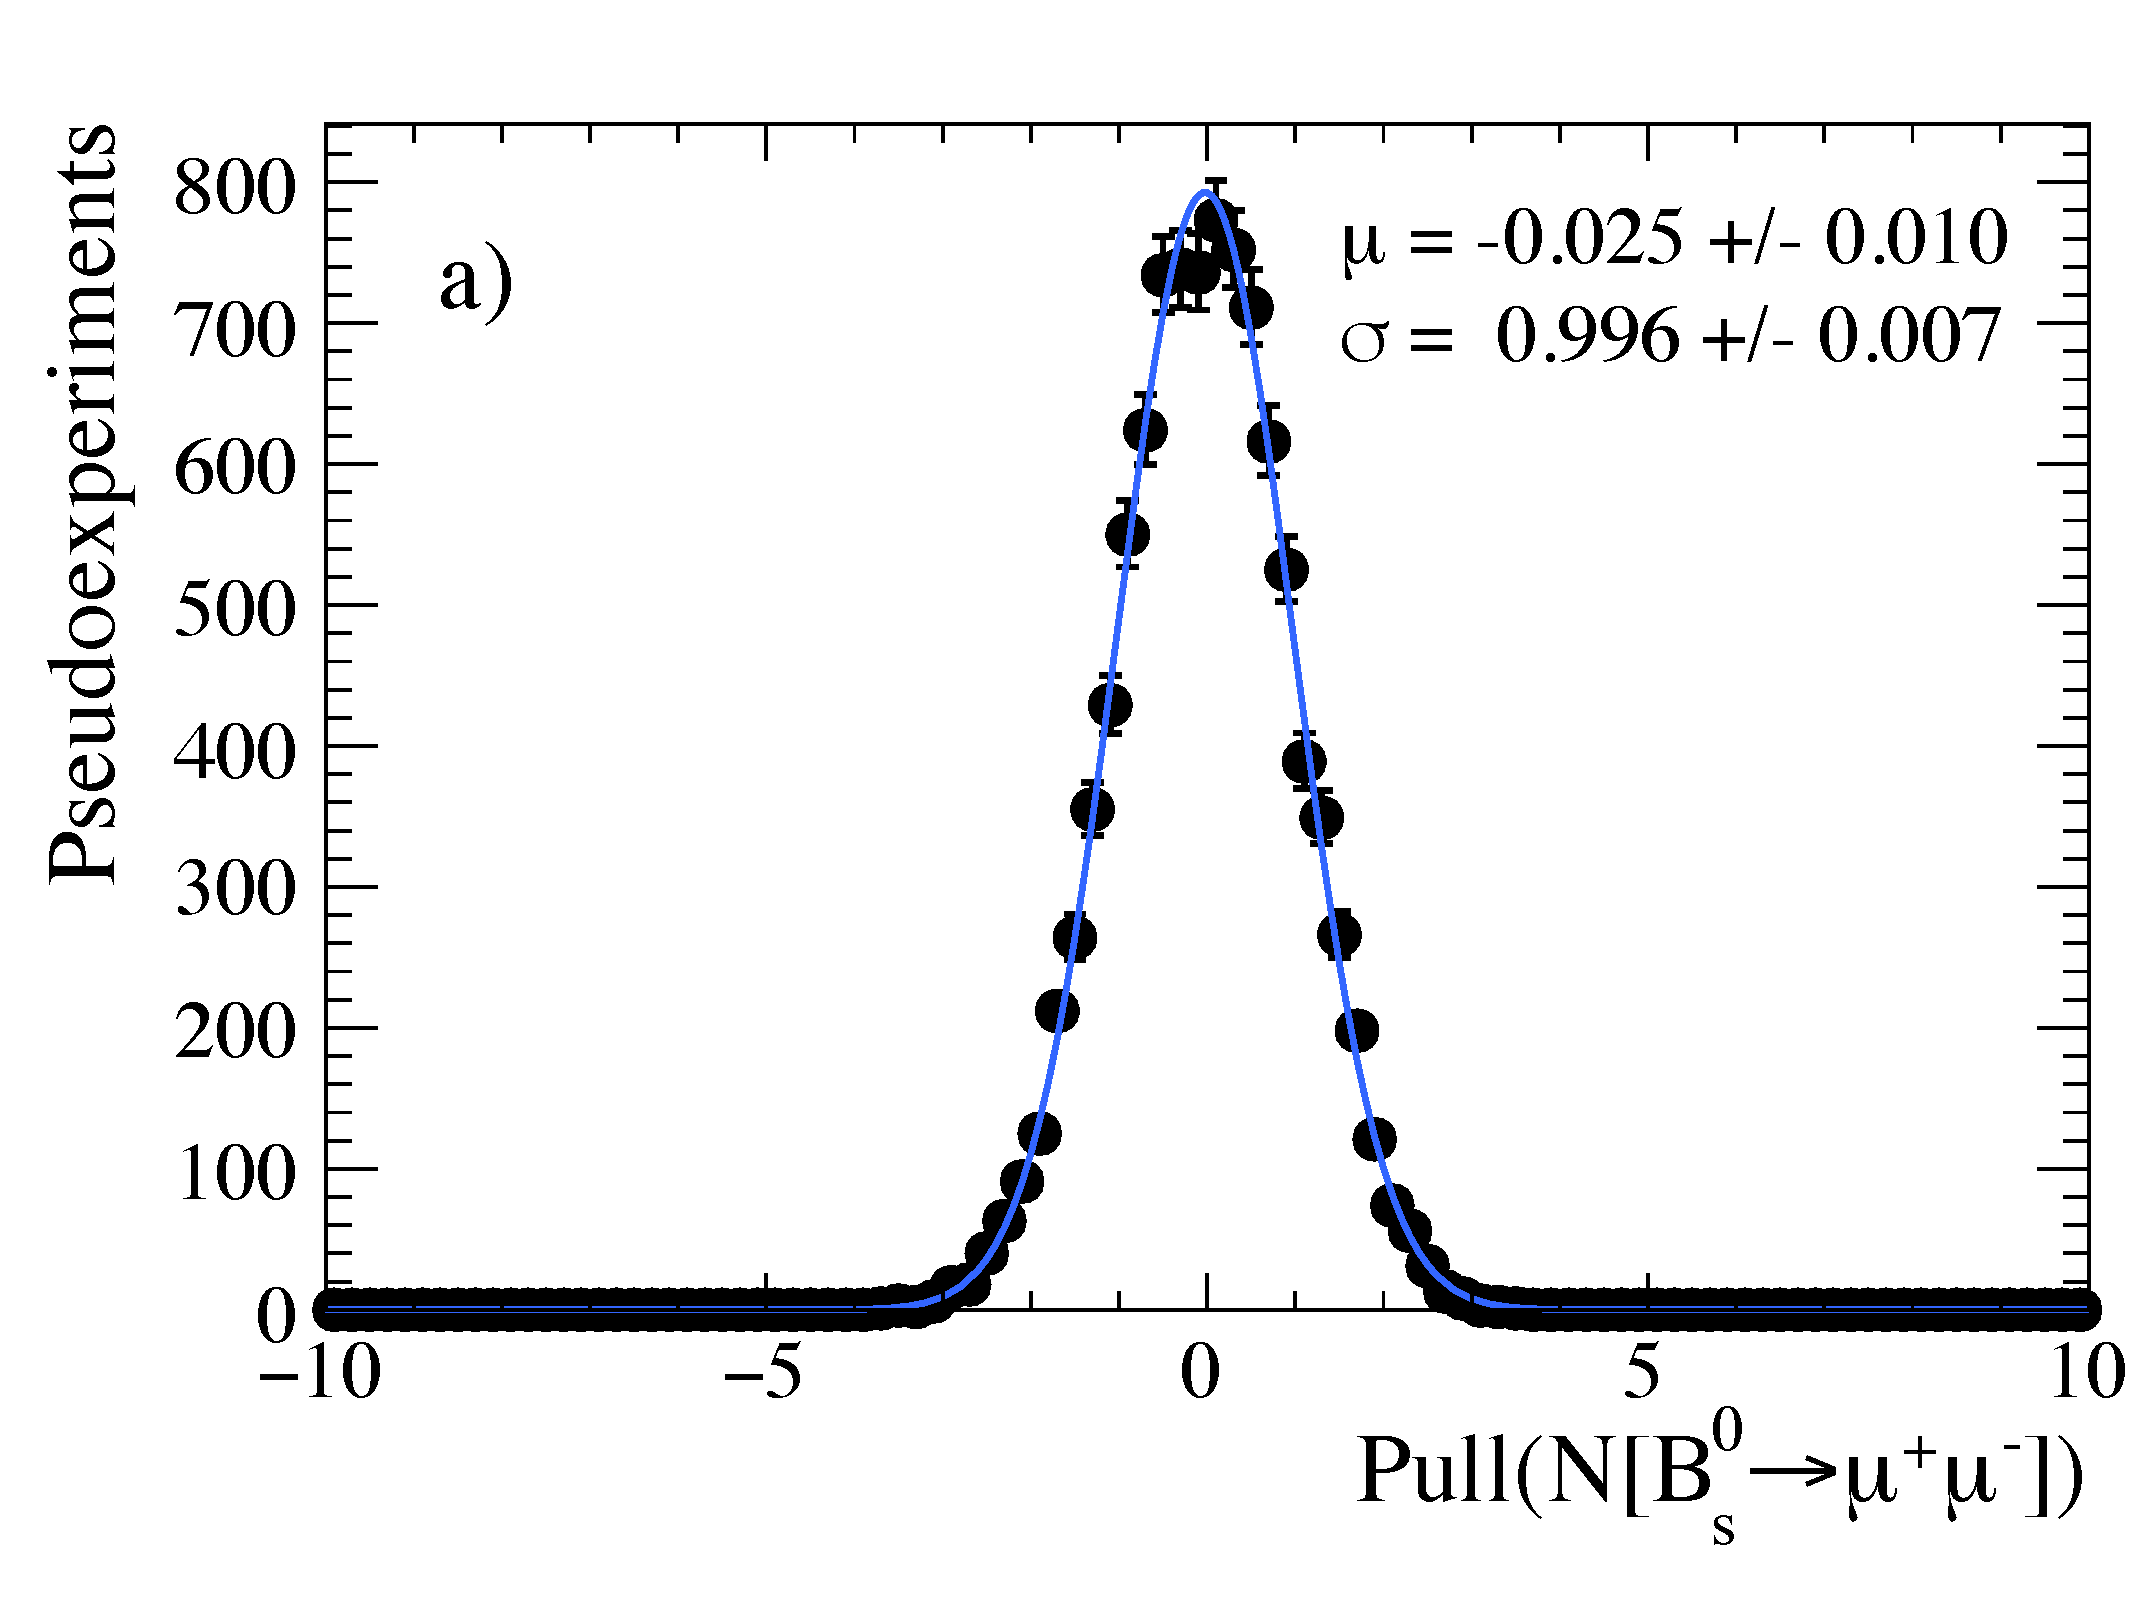
\includegraphics[width=0.49 \textwidth]{./Figs/LifetimeSystematics/Bs2MuMu_yield_pull_50fb.pdf}
        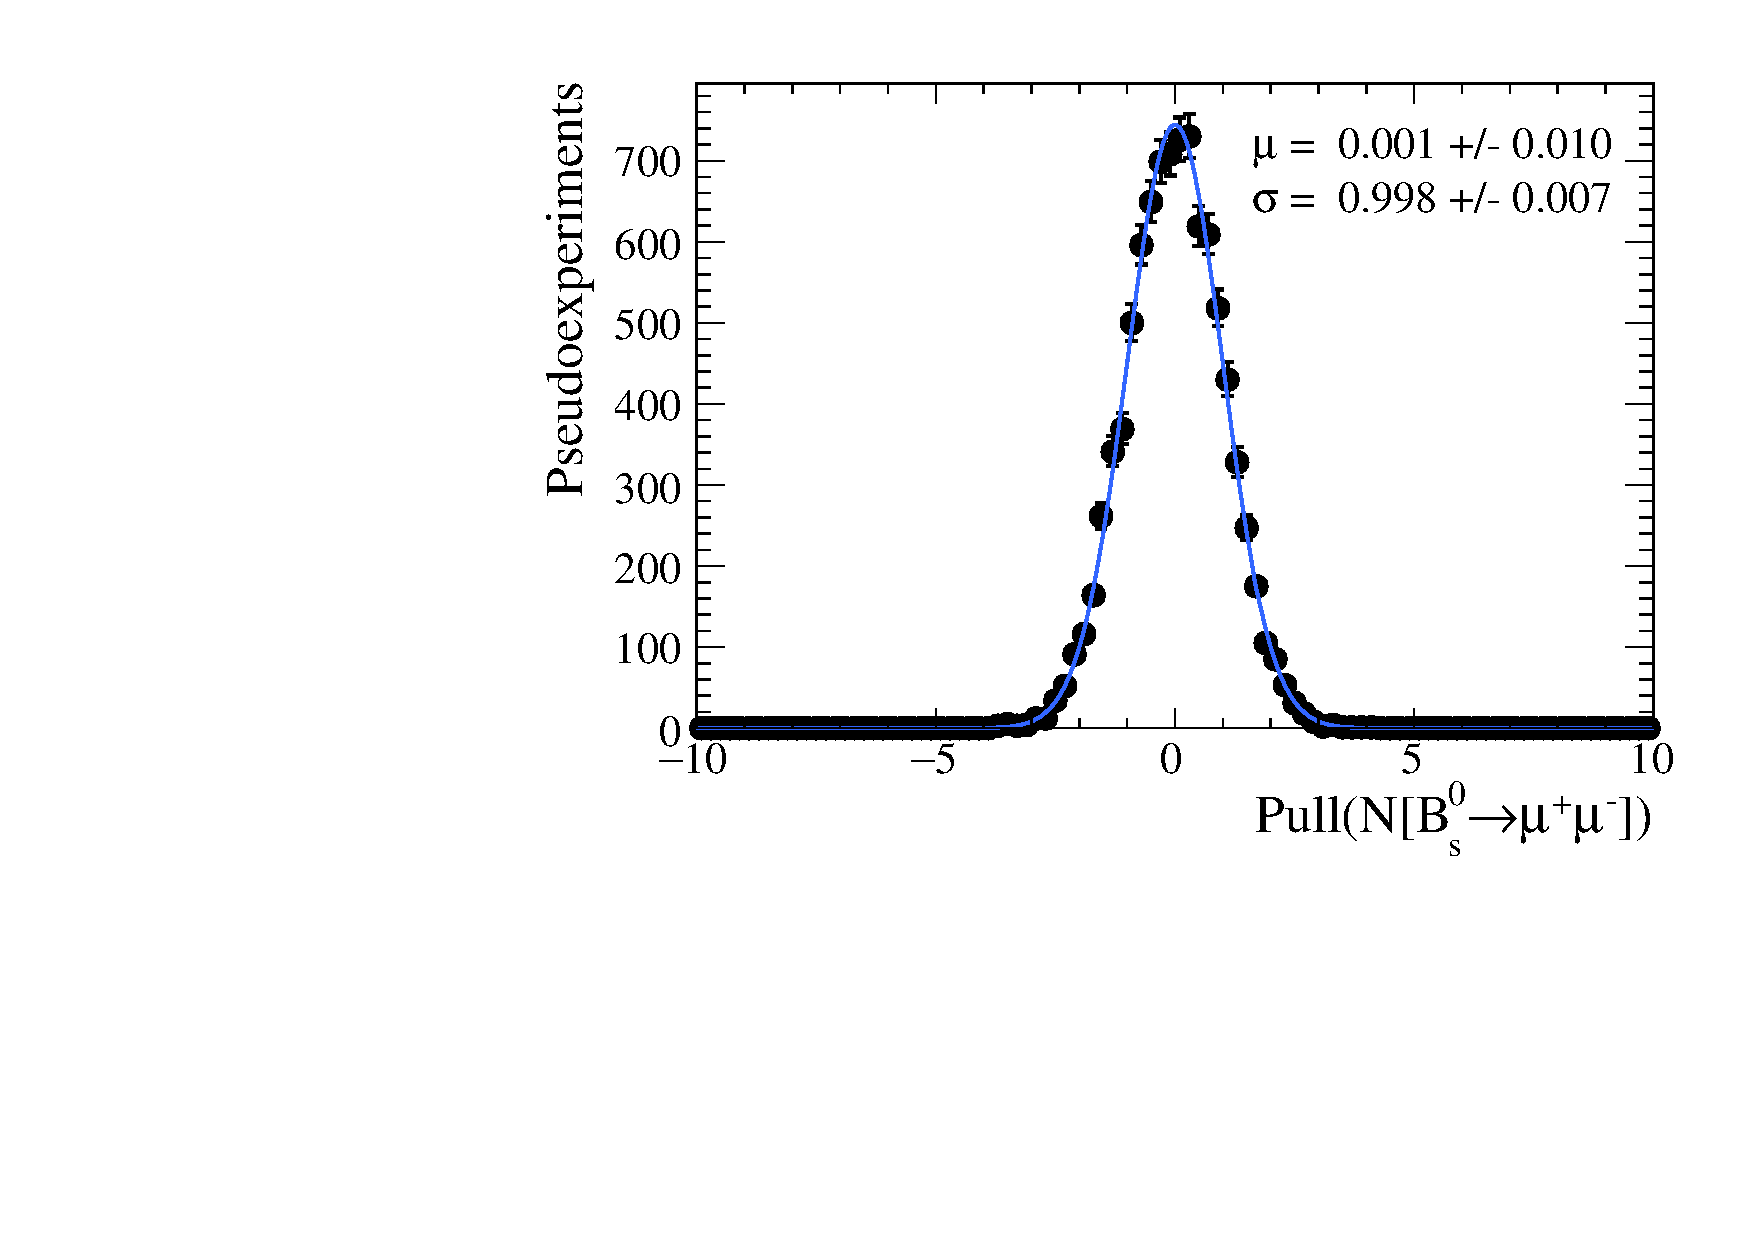
\includegraphics[width=0.49 \textwidth]{./Figs/LifetimeSystematics/Bs2MuMu_yield_pull_300fb.pdf}
    \caption{Pull distribution for \bsmumu measured yields from toy studies with 50 and 300 \fb.}
    \label{fig:BsmumuYieldPulls}
\end{figure}


\subsection{Overall bias on \tmumu and \Gmumu}
The remaining area of the fit to investigate is any underlying bias in the fit on the measured values of \tmumu and \Gmumu. (As discussed in Section~\ref{} the pull distribution for the measured effective lifetime is biased for the expected number of statistics but the pull distribution for \Gmumu produces a mean and width consistent with 0 and 1, respectively. However the coverage of the uncertainties of both \mmumu and \Gmumu are reasonable and the biased \tmumu pull arises from the likelihood function as discussed in Section~\ref{sec:tauORinvtau}. 

The overall bias in the fit for measuring \tmumu and \Gmumu is evaluated from the difference between the measured and generated values from toy studies. A total of 10,000 toy studies are performed generating only \bsmumu and combinatorial background decays so the fit bias is not masked by contamination from mis-identified backgrounds.  The bias arising from the small contribution of mis-identified backgrounds in the mass range of the fit is evaluated in Section~\ref{}. The difference between the measured and generated \tmumu and \Gmumu values is evaluated for toy studies for the expected and observed number of \bsmumu decays. The fit bias is evaluated for the observed number of decays because these are fewer than expected. The resulting distributions are shown in Figure~\ref{}. The mean of the \Gmumu difference distribution is consistent with 0 and the mean of the \tmumu difference distribution is 0.03 \ps for the observed number of decays.  Therefore giving a systematic uncertainty of 0.03ps for the fit accuracy of \tmumu and no systematic uncertainty for \Gmumu.

\begin{figure}[htbp]
    \centering
        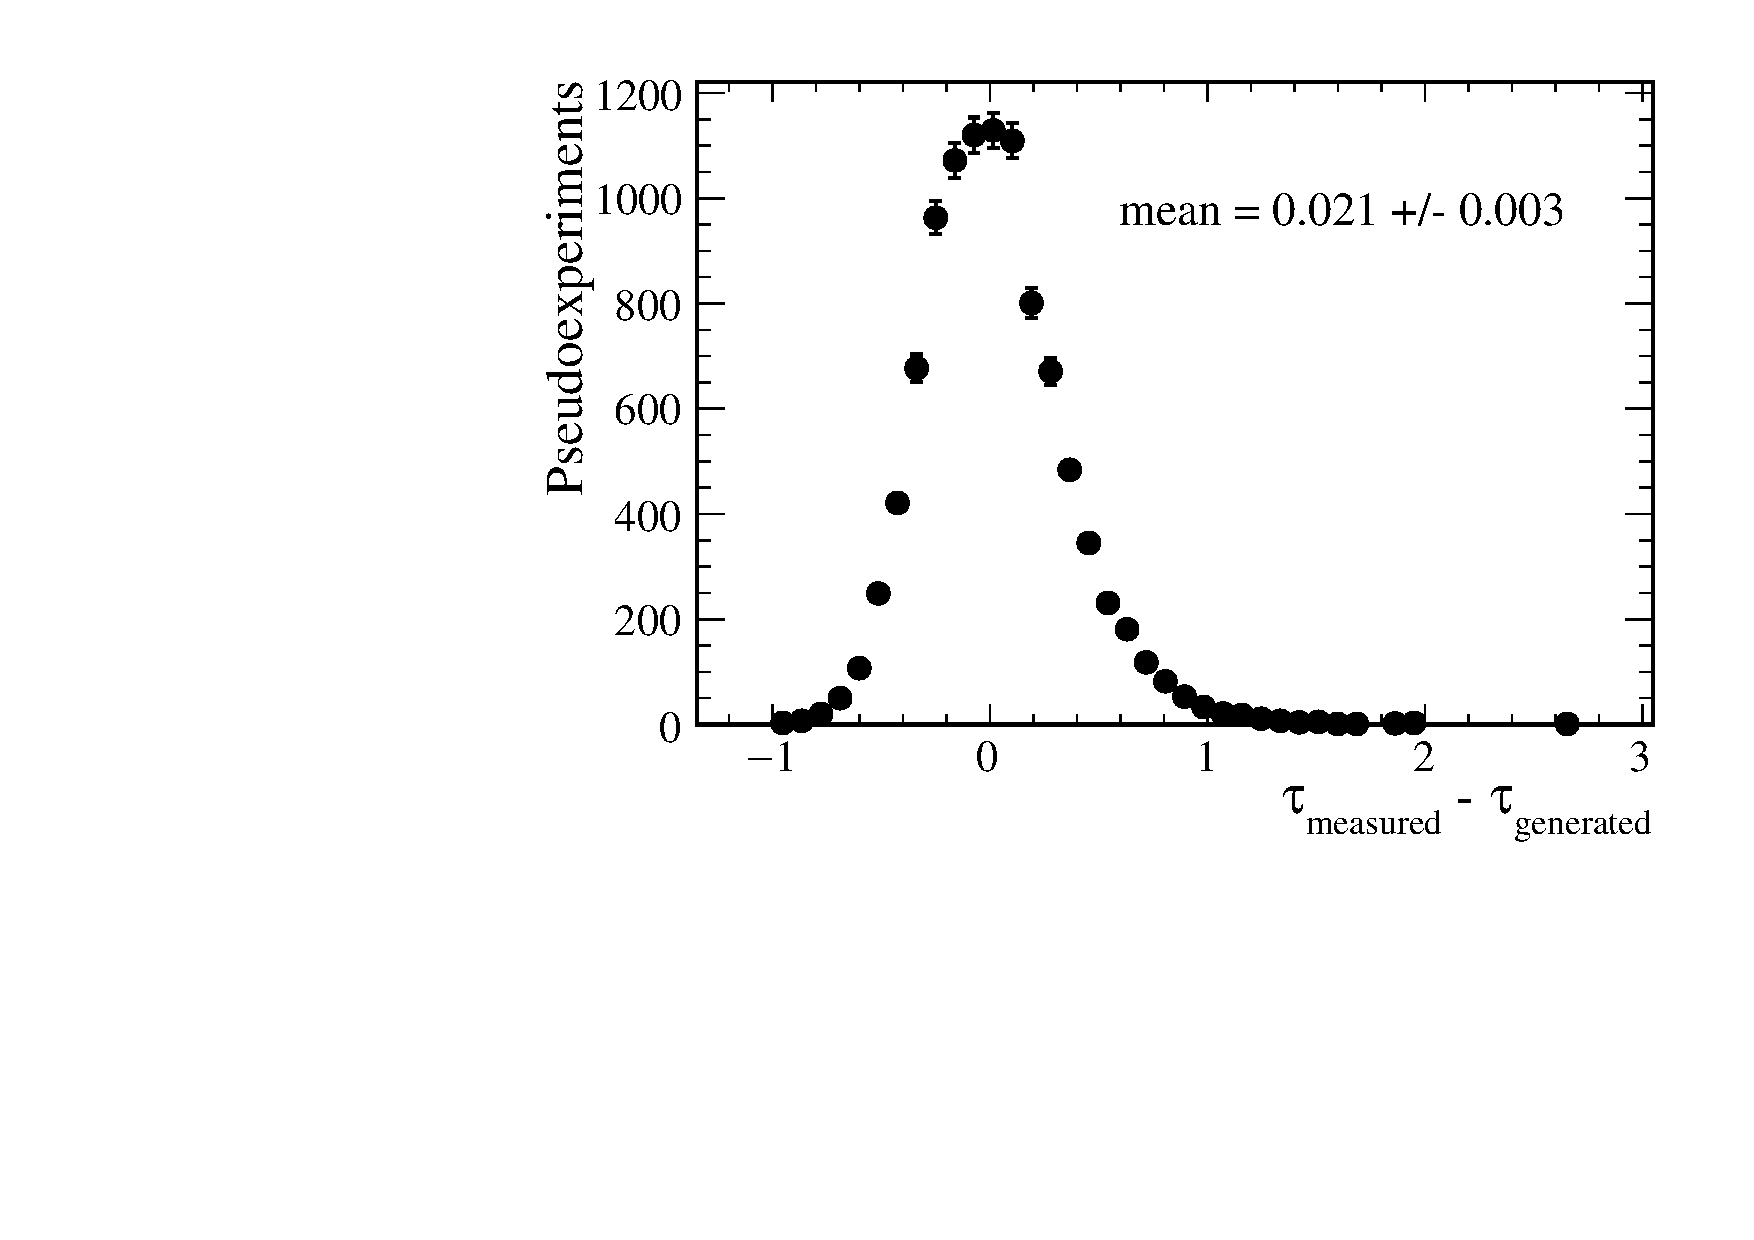
\includegraphics[width=0.49 \textwidth]{./Figs/LifetimeSystematics/tau_meas-tau_gen_expected.pdf}
        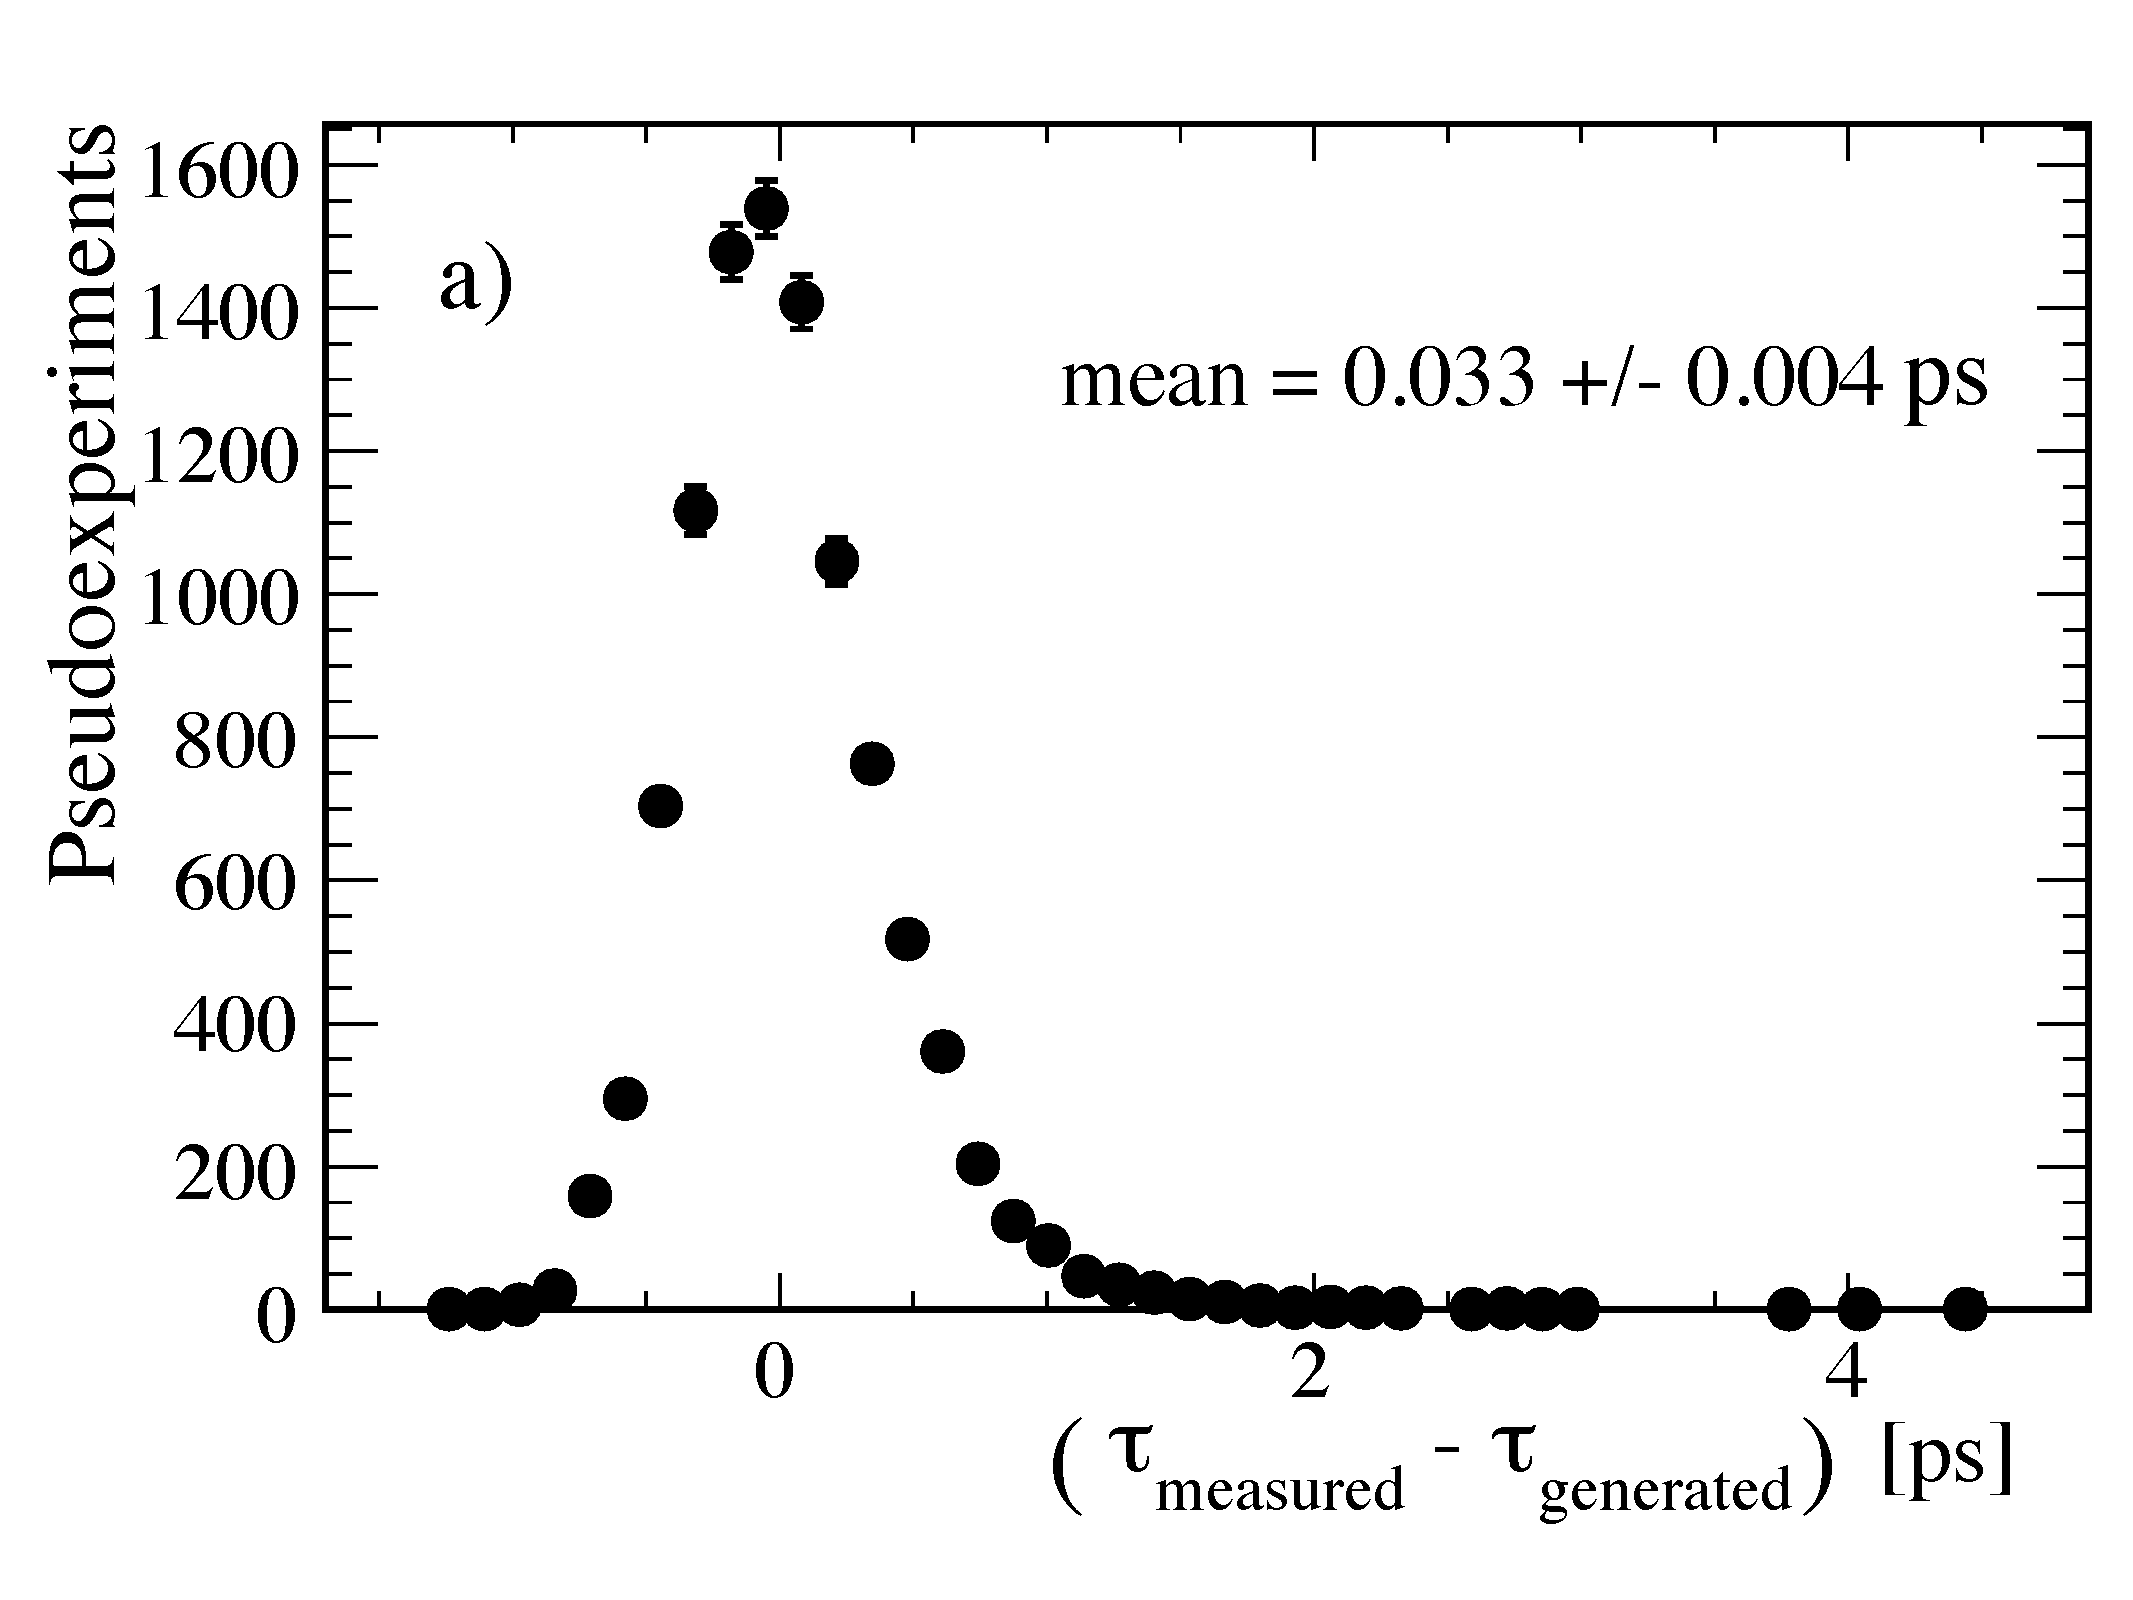
\includegraphics[width=0.49 \textwidth]{./Figs/LifetimeSystematics/tau_meas_tau_gen_observed.pdf}
    \caption{Overall bias in \tmumu, evaluated as the difference between the measured, $\tau_{measured}$, and the generated, $\tau_{generated}$, lifetimes for toy studies using the expected (left) and observed (right) \bsmumu and combinatorial background yields.}
    \label{fig:BsmumuYieldPulls}
\end{figure}


\section{Background contamination}
\label{sec:BKGcontaim}
The mass fit configuration used to measure the \bsmumu effective lifetime only includes components for \bsmumu and combinatorial background decays and only candidates with a \bs mass between 5320 - 6000 \mevcc are used in the mass fit. Although the majority of background decays from mis-identified semi-leptonic and \bhh decays and \bdmumu decays fall outside this mass window, as shown in Figure~\ref{fig:toygen} the tails of some backgrounds still end up in the mass window. The backgrounds that need to be considered are \bdmumu, \bhh, \lambdab, \bdpimunu, \bsKmunu, \bupimumu, \bdpimumu, \bcjpsimunu, with \bhh, \bdmumu and \lambda being of particular importance. 

The number of expected background decays and their mass \pdfs in the mass range 4900 - 6000 \mevcc were computed using the methods described in Chapter~\ref{sec:BFanalysis}. The number of decays from each background type expected in the smaller mass range 5320 - 6000 \mevcc are computed by integrating the mass \pdfs. The expected yields for each background in both mass ranges are given in Table~\ref{tab:tabC}. The expected yields are all $<$ 1 for each background source. 
\begin{table}[htbp]
\begin{center}
\begin{tabular}{lcc}
\hline
Decay & \multicolumn{2}{c}{Expected yield in mass range} \\ 
 & 4900 - 6000 \mevcc & 5320 - 6000 \mevcc \\ \hline
\bsmumu & 30.9 & 30.5 \\ 
\bdmumu & 3.3& 0.2\\ 
\bhh & 9.7& 0.9\\ 
\lambdab &  13.3 & 0.6\\ 
\bdpimunu & 40.5 & 0.1 \\ 
\bsKmunu &  9.1 & 0.0\\ 
\bupimumu &  6.0 & 0.0\\ 
\bdpimumu  &  4.9 & 0.6\\ 
\bcjpsimunu  &  9.8 & 0.0\\ 
Combinatorial background & 66.2 & 40.6\\ 
\hline
\end{tabular}
\vspace{0.7cm}                                                                                                                                               
\caption{Number of expected decays in data passing the \bsmumu effective lifetime selection in the mass ranges 4900 - 6000 \mevcc and 5320 - 6000 \mevcc.}
\label{tab:tabC}
\end{center}
\vspace{-1.0cm}                                                                                                                                               
\end{table}

The impact of backgrounds not modelled in the mass fit on the measured lifetime and inverse lifetime is evaluated using two sets of toy studies. The toy studies have the same general set up as described in Section~\ref{sec:toys}. One set of toy studies assumes there are no background other than the combinatorial background and therefore only \bsmumu and combinatorial background candidates are generated. The second set of toy studies generates all possible background decays. The expected yields are fluctuated using a Poisson distribution around their expected values to 1 decimal place. For each configuration 10,000 toy studies were performed and the pull distributions for \Gmumu of each toy set up is compared. The pull distributions for \tmumu are not used due to their non-Gaussian distribution disused in Section~\ref{sec:tauORinvtau}. 

The inclusion of all the background decays causes a shift in the mean of the \Gmumu pull distribution of 0.025 \ps$^{-1}$ as shown in Figure~\ref{fig:bkdcontam}. Therefore, assuming the expected uncertainty in Section~\ref{sec:toyresults} of 0.28 \ps for \tmumu the systematic shift from not including all backgrounds in the fit configuration is 0.007 \ps.% for \tmumu and Y for \Gmumu. 

\begin{figure}[htbp]
    \centering
        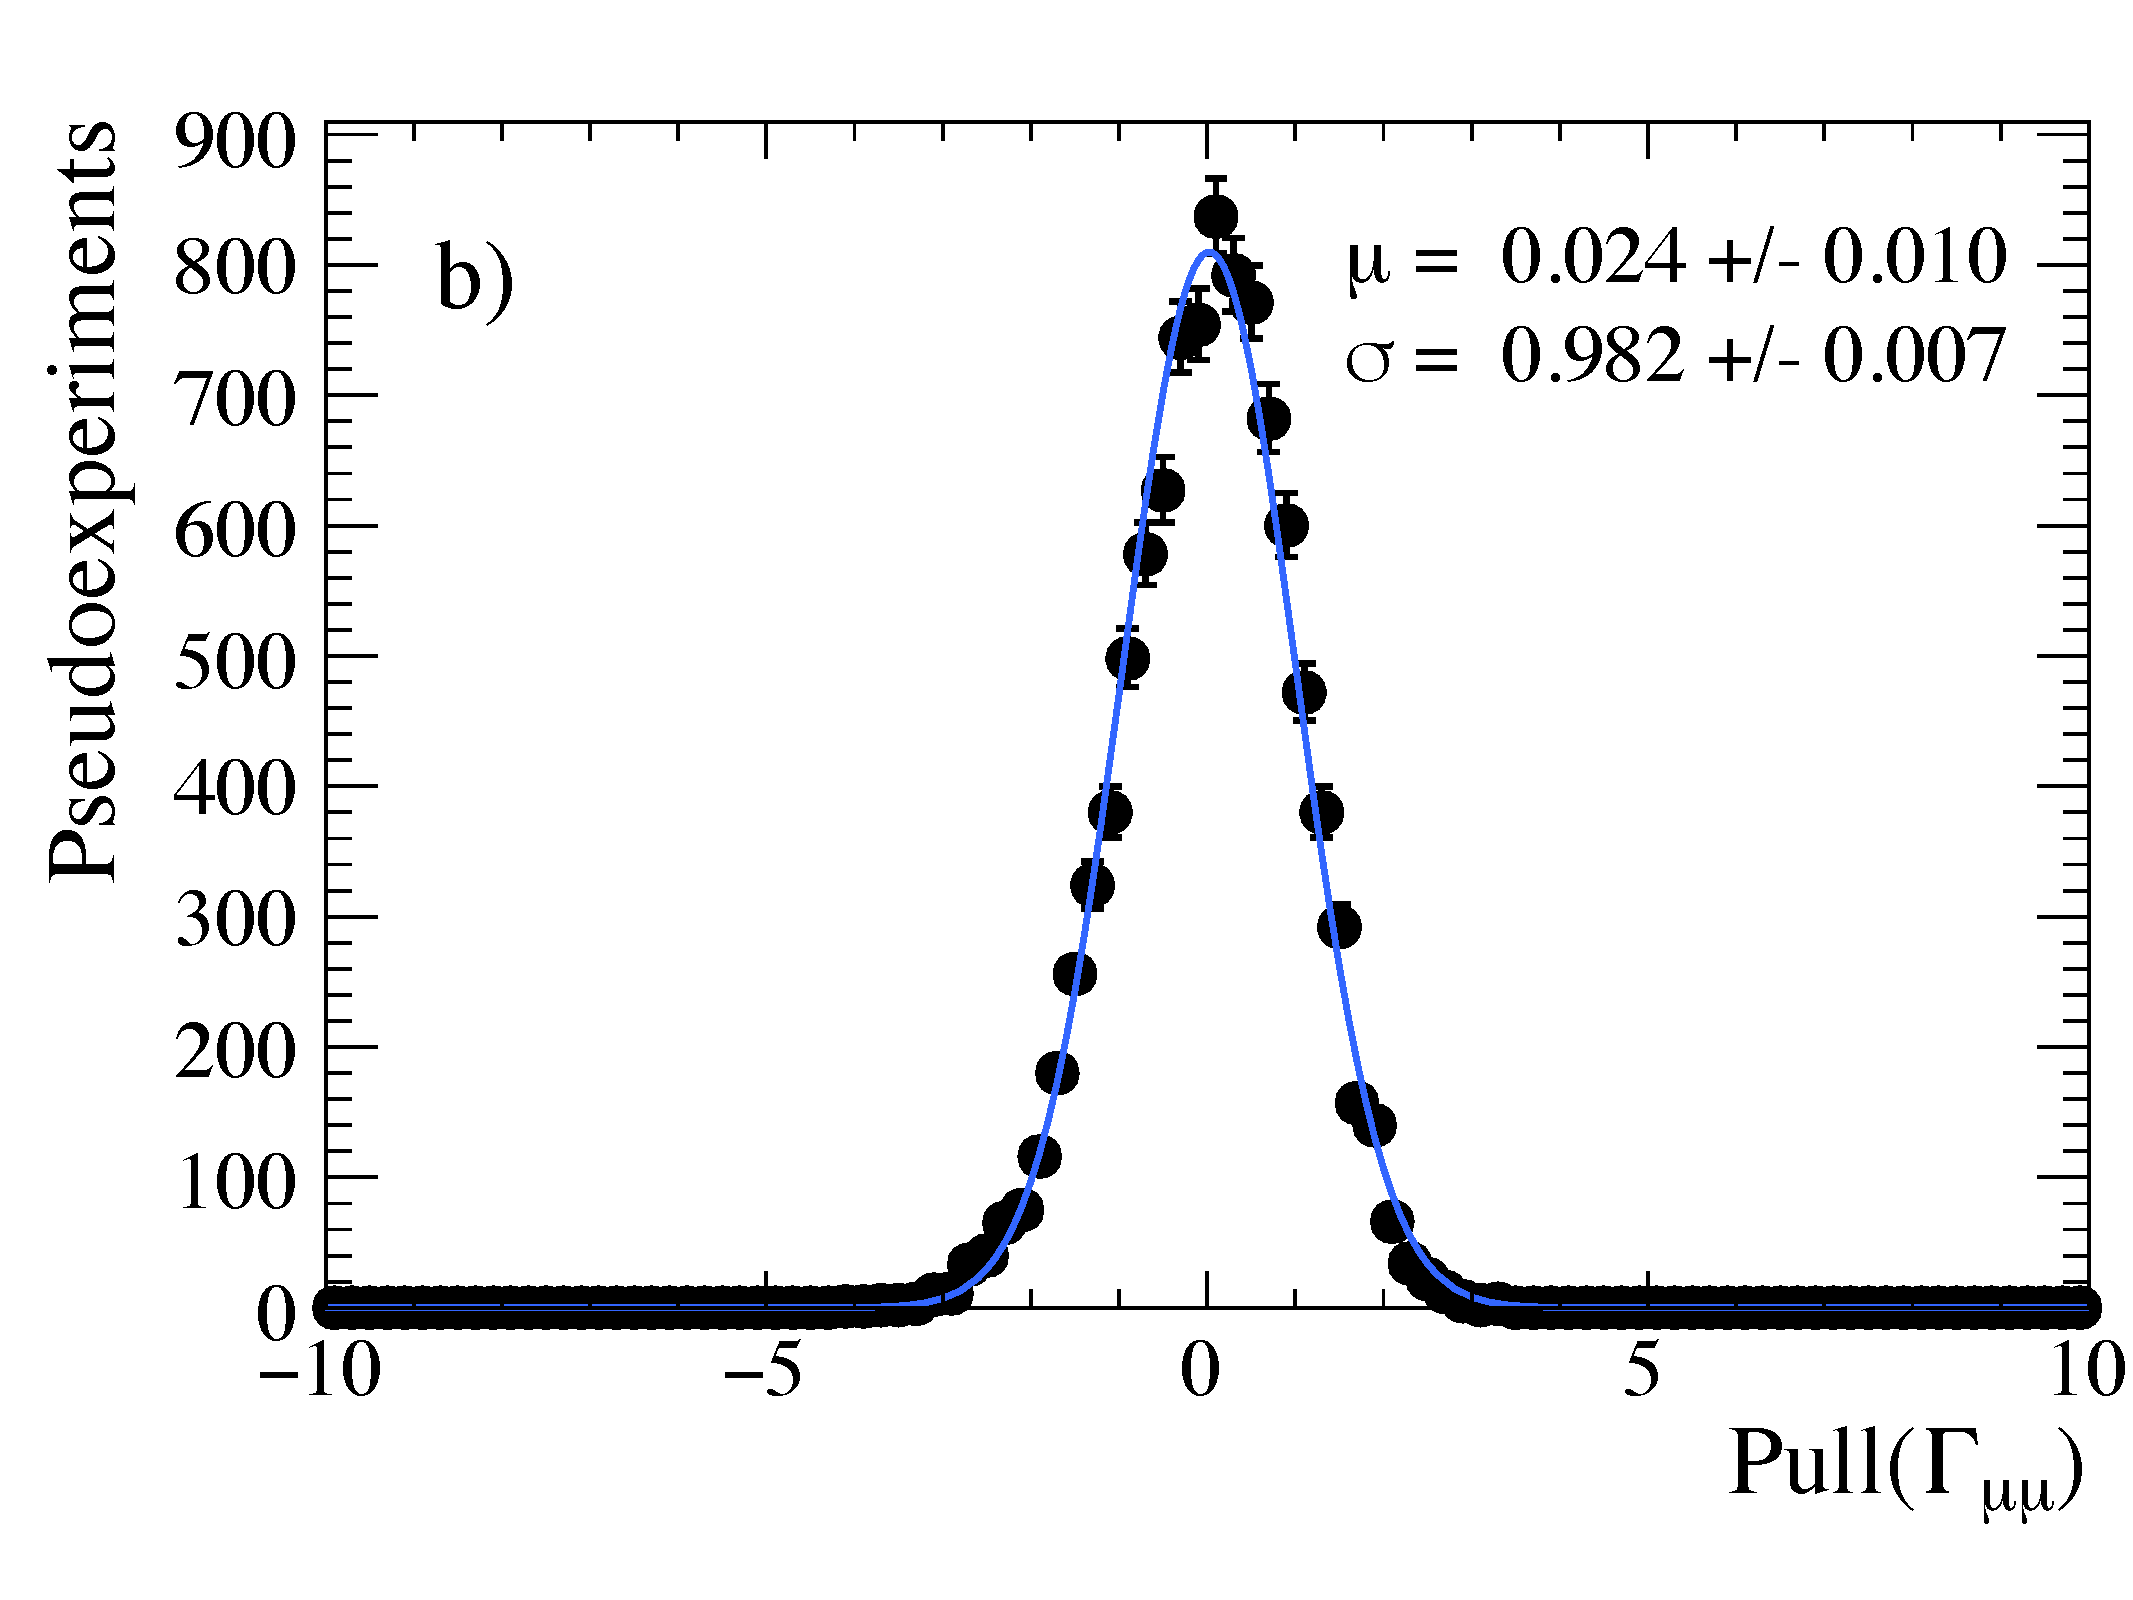
\includegraphics[width=0.49 \textwidth]{./Figs/LifetimeSystematics/5320_all_bkgnds_gamma_pull_CKM.pdf}
        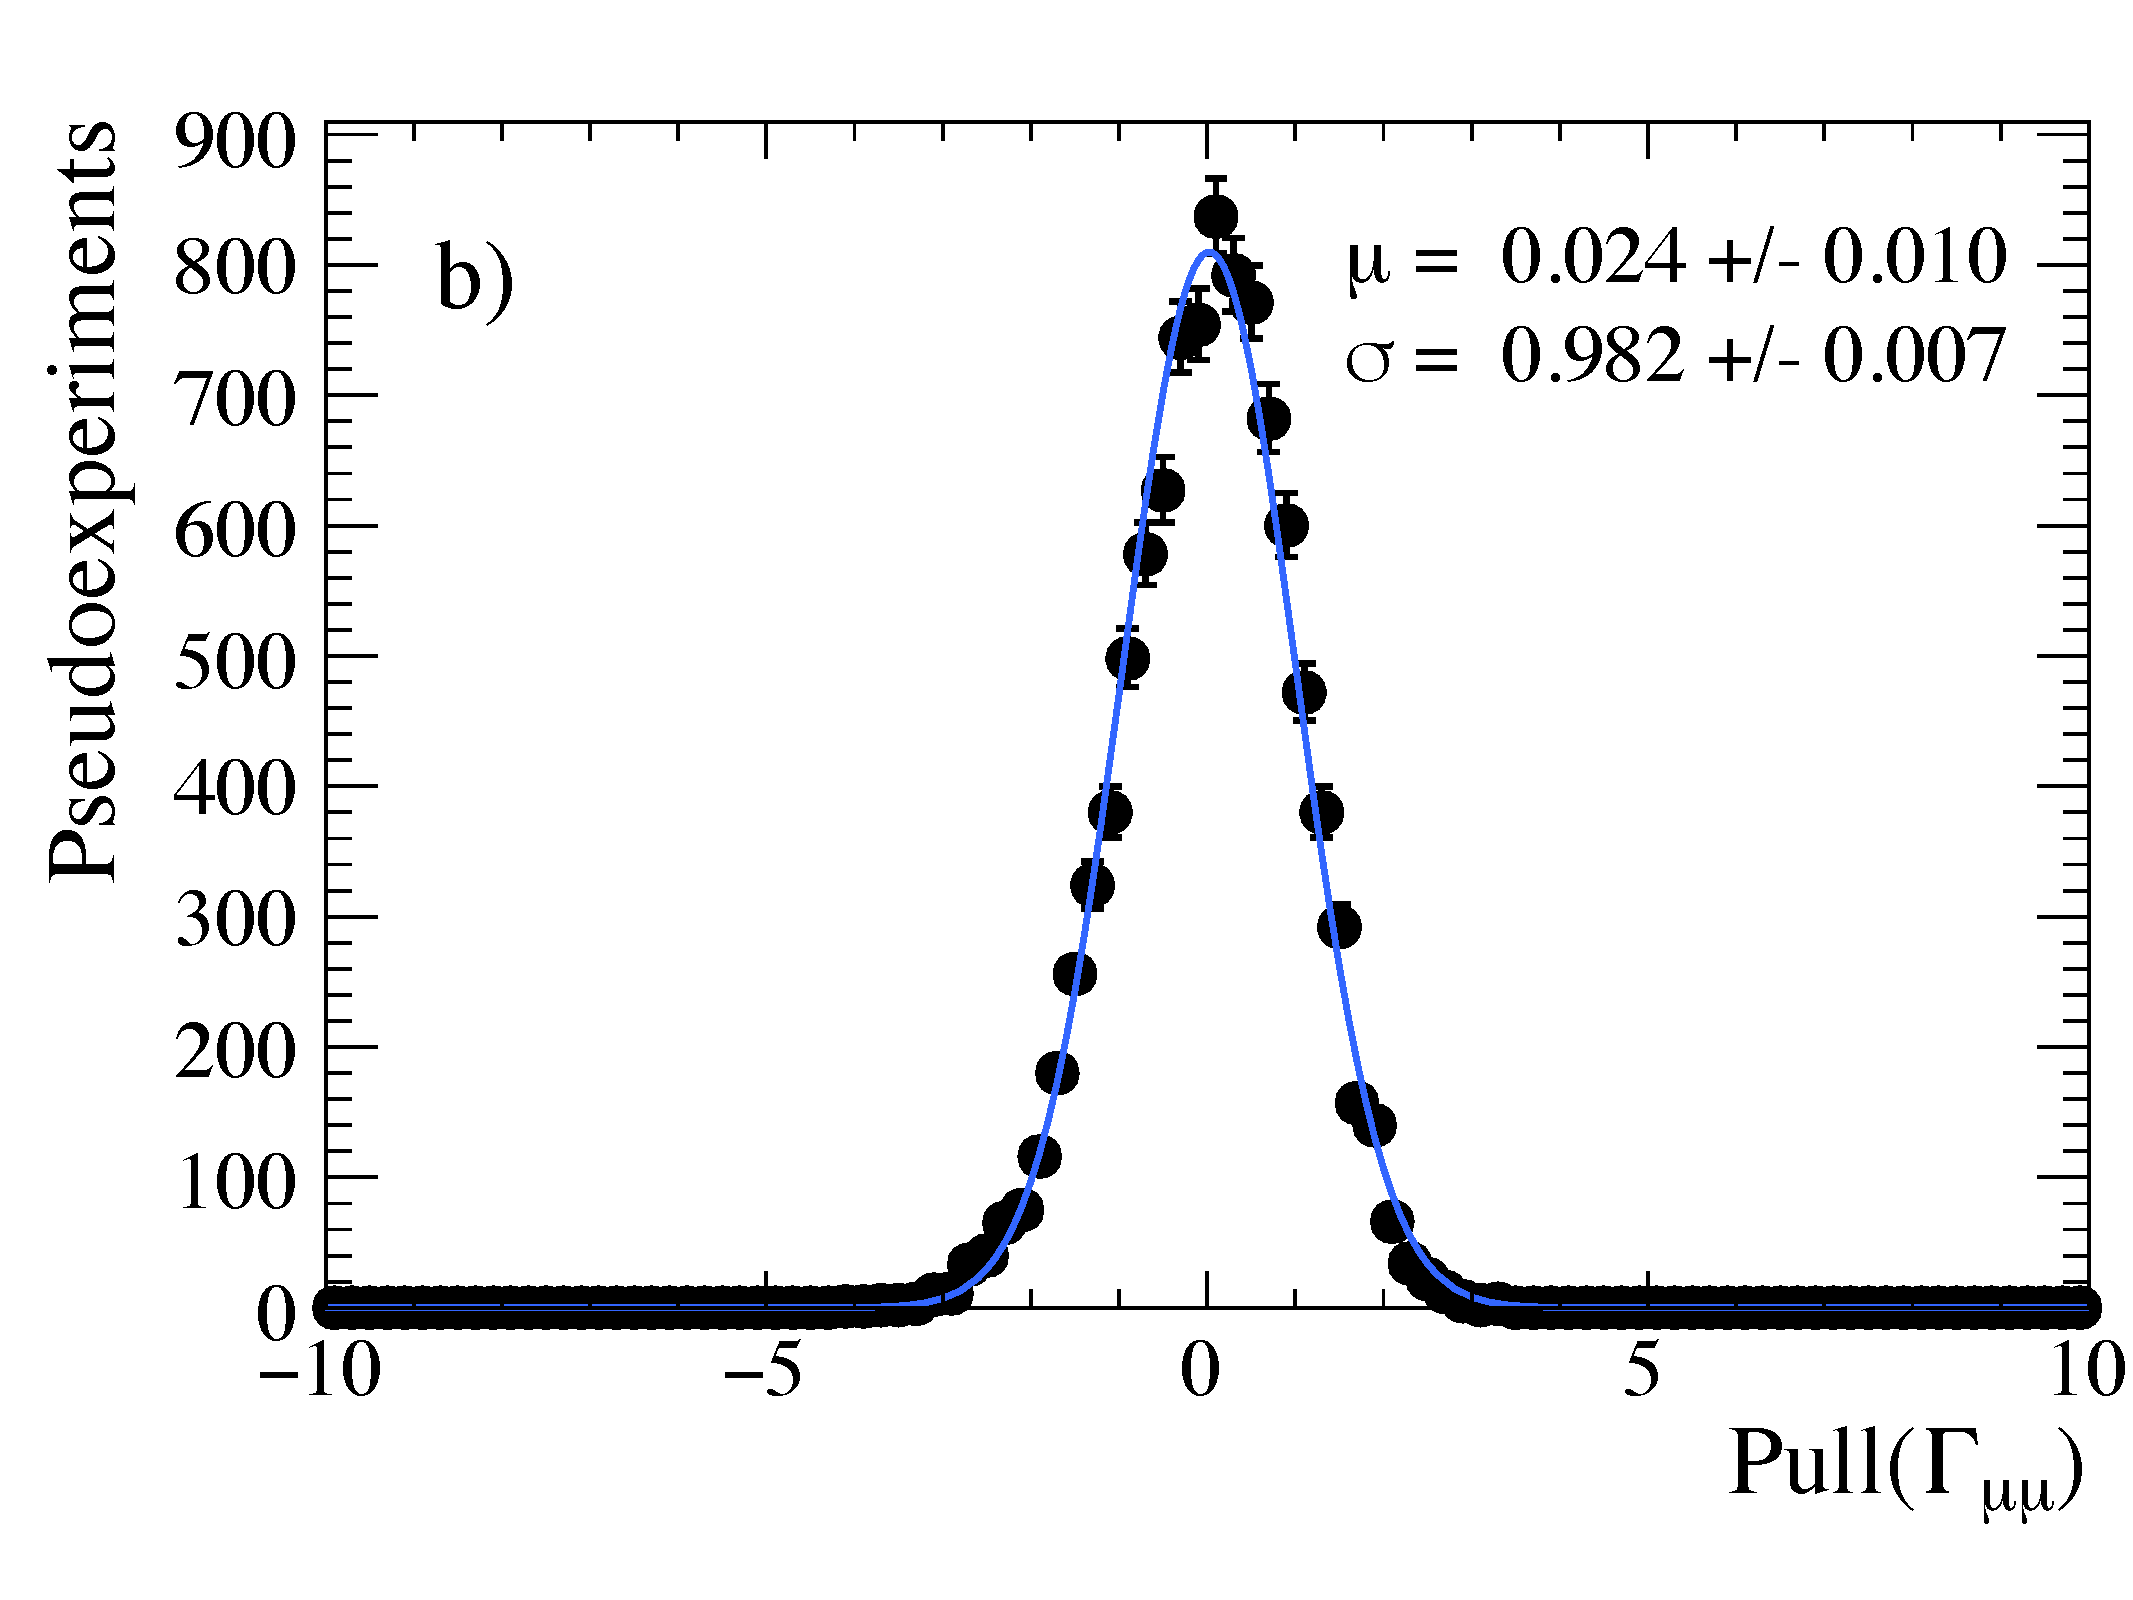
\includegraphics[width=0.49 \textwidth]{./Figs/LifetimeSystematics/5320_all_bkgnds_gamma_pull_CKM.pdf}
    \caption{Pull distribution for \Gmumu from 10,000 toy studies ....}
    \label{fig:bkdcontam}
\end{figure}

The expected number of \bsmumu and \bdmumu decays assumes the Standard Model branching fraction, however the current world averages (excluding the results presented in Chapter~\ref{sec:BFanalysis}) are different and the expected number of \bsmumu decays decreases and the expected number of \bdmumu decays increases, the changes in the yields are given in Table~\ref{tab:tabD}. The toy studies were repeated with the world average but the shift in the mean of the pull distribution was smaller, therefore the larger value from the SM predictions are used.
\begin{table}[htbp]
\begin{center}
\begin{tabular}{lcc}
\hline
Decay & \multicolumn{2}{c}{Expected yield in 5320 - 6000 \mevcc} \\ 
 & Standard Model & World average \\ \hline
\bsmumu & 30.5 & 22.5 \\ 
\bdmumu & 0.2& 0.7\\ 
\hline
\end{tabular}
\vspace{0.7cm}                                                                                                                                               
\caption{Number of expected decays in data passing the \bsmumu effective lifetime selection in the mass range 5320 - 6000 \mevcc, using the Standard Model and world average branching fraction values.}
\label{tab:tabD}
\end{center}
\vspace{-1.0cm}                                                                                                                                               
\end{table}

\subsection{Mass \pdf parameters}
\label{sec:massPDFsyst}
The data collected in Run~1 and Run~2 are combined for the measurement of the \bsmumu effective lifetime and the mass and decay time fits are applied to the combined data. However the parameters used in the mass \pdf in Table~\ref{} were evaluated specifically for Run~1 data and different parameters are available for Run~2 data. Therefore the influence of the choice of mass \pdf parameters on the measured \tmumu and \Gmumu values must be evaluated. 

Toy studies are performed to understand the size of the impact of the mass fit choice on the effective lifetime measurement. Only \bsmumu and combinatorial background decays are generated to separate mass \pdf effects from the contamination of mis-identified backgrounds and \bdmumu decays in the mass window. \bsmumu candidates are generated using the Run~1 parameters in Table~\ref{} but the mass fit is performed using the Run~2 parameters in Table~\ref{}. The pull distribution for 10,000 toy studies of \Gmumu from this configuration are compared with those from toy studies where Run~1 parameters are used to generate and fit the mass distribution. The change in the measured lifetime with the mass \pdf parameters is negligible as shown in Figure~\ref{fig:masspdfsyst} that overlays the pull distributions for the two toy configurations studied. Therefore no systematic uncertainty is assigned. 

\begin{figure}[htbp]
    \centering
        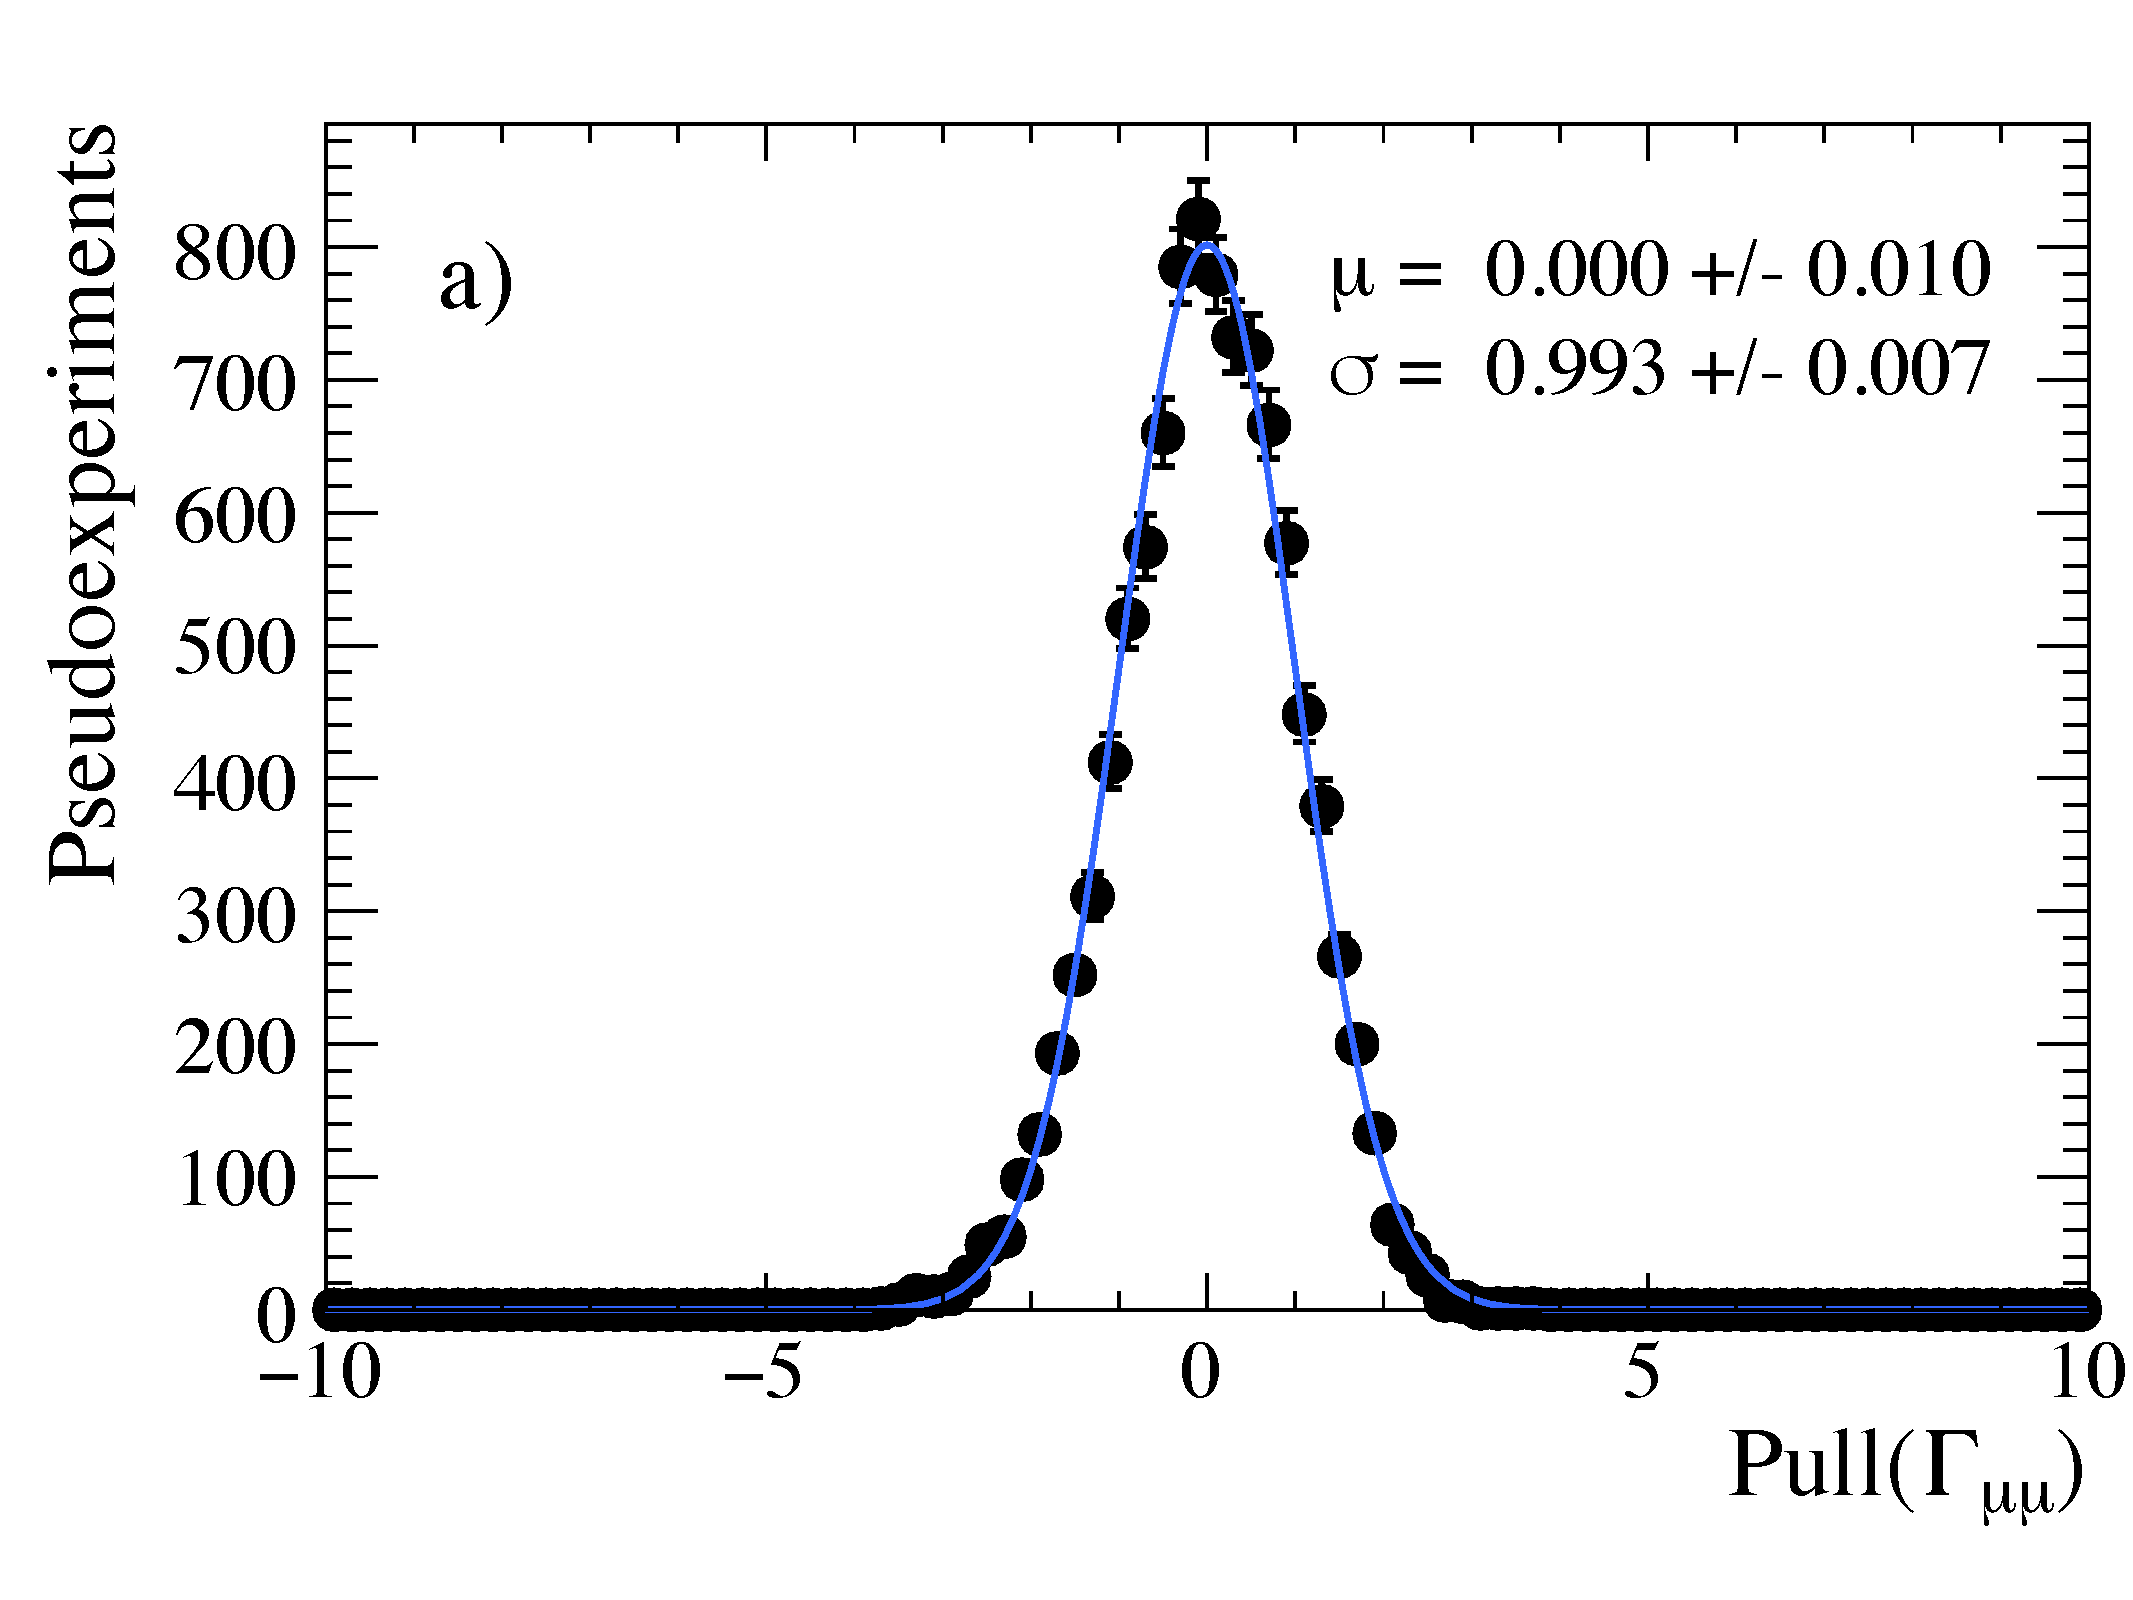
\includegraphics[width=0.49 \textwidth]{./Figs/LifetimeSystematics/Gamma_pull_mass_pdf_Run1.pdf}
        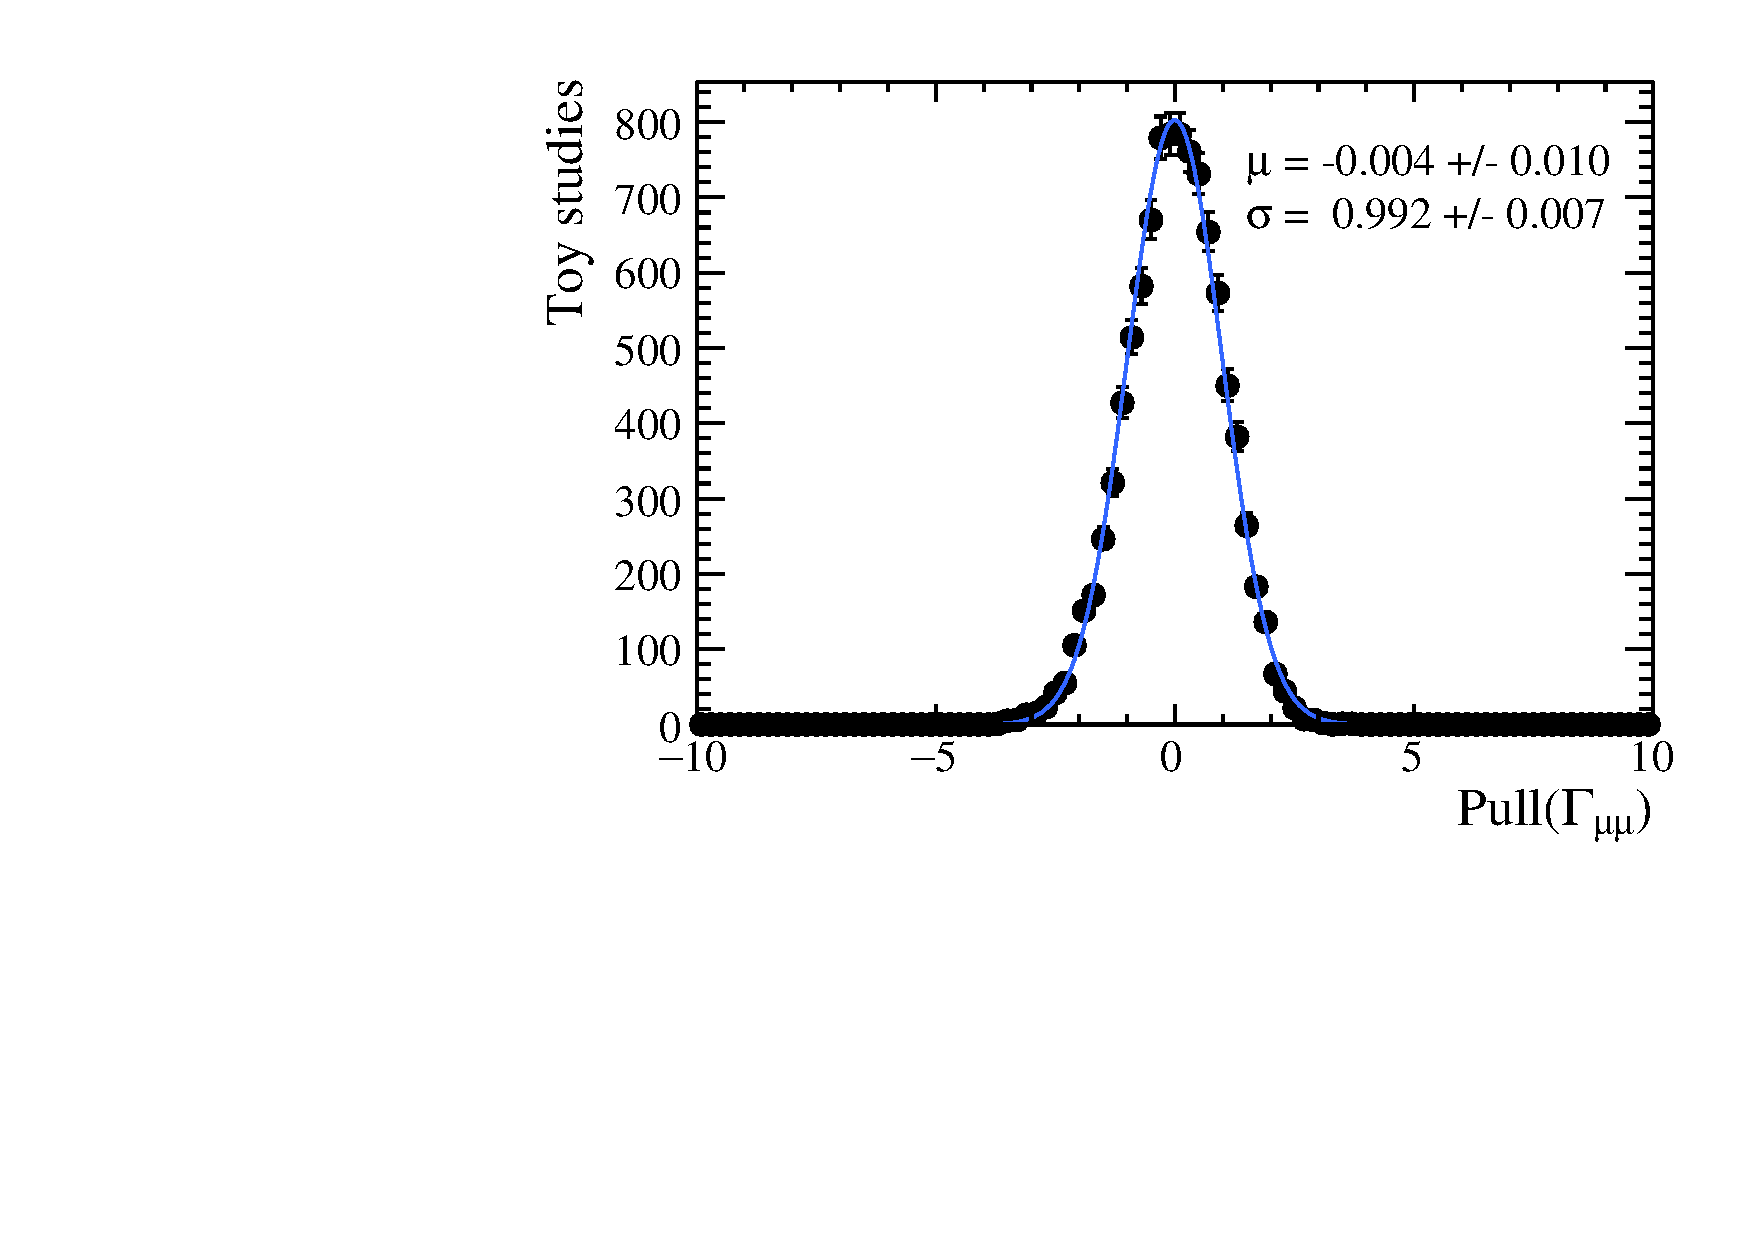
\includegraphics[width=0.49 \textwidth]{./Figs/LifetimeSystematics/Gamma_pull_mass_pdf_Run2.pdf}
    \caption{Pull distribution for \Gmumu from 10,000 toy studies where the \bsmumu mass distribution is generated using the Run~1 parameters in Table~\ref{} and the mass fit is performed using Run~1 parameters (left) and Run~2 parameters (right).}
    \label{fig:masspdfsyst}
\end{figure}


\subsection{Acceptance function accuracy}
\label{sec:accptsyst}
The decay tie acceptance comes from weighted simulated decays. This relies on the assumption that the weighted simulated decays model the data reasonable well. To test this assumption, as well as the strategy used to measure the \bsmumu effective lifetime, the lifetime of the more abundant \bdkpi and \bskk decays are measured.

\bdkpi decays have a much larger branching fraction the \bsmumu decays at XXX and are therefore more abundant in data. The selection requirements used to identify these decays in 2011, 2012, 2015 and 2016 data are detailed in Chapter~\ref{} and are kept very similar to the \bsmumu selection. All candidates are required to be TIS, although this considerably reduces the statistics, \bhh triggers are $\%$ efficient, the TIS triggers are relatively unbiased with respect to the decay time similarly to triggers that select \bsmumu decays. Whereas TOS triggers that identify \bhh decays create a large bias on the decay time distribution due to the dependence on the trigger lines on IP, IP \chisqd and flight distance variables. The DLL$_{K\pi}$ variable is used to separate \bdkpi decays from other \bhh decays, as detailed in Section~\ref{} and candidates are reconstructed with the daughter with the highest DLL$_{K\pi}$ value assigned the kaon mass hypothesis and the daughter particle with the lowest DLL$_{K\pi}$ value the pion mass hypothesis.

The measurement of the \bdki lifetime is performed in the same way as the \bsmumu effective lifetime measurement and all years of data are combined into one data set. An extended, unbinned maximum likelihood fit is performed to the \bdkpi mass distribution. Components for \bdkpi, \bskpi and combinatorial background decays are included in the mass fit. Both B meson decays are modelled by Crystal Ball functions with parameters taken from some source. Combinatorial background decays are modelled by an exponential function with the slope left free in the mass fit. The mass fit, shown in Figure~\ref{fig:bdkpimassfit}, is used to calculate sWeighted that are re-normalised using equation~\ref{}. The lifetime, $\tau_{K\pi}$, and the inverse lifetime $\Gamma_{K\pi}$, are measured from an unbinned maximum likelihood fir to the sWeighted decay time distribution. 

\begin{figure}[htbp]
\centering
  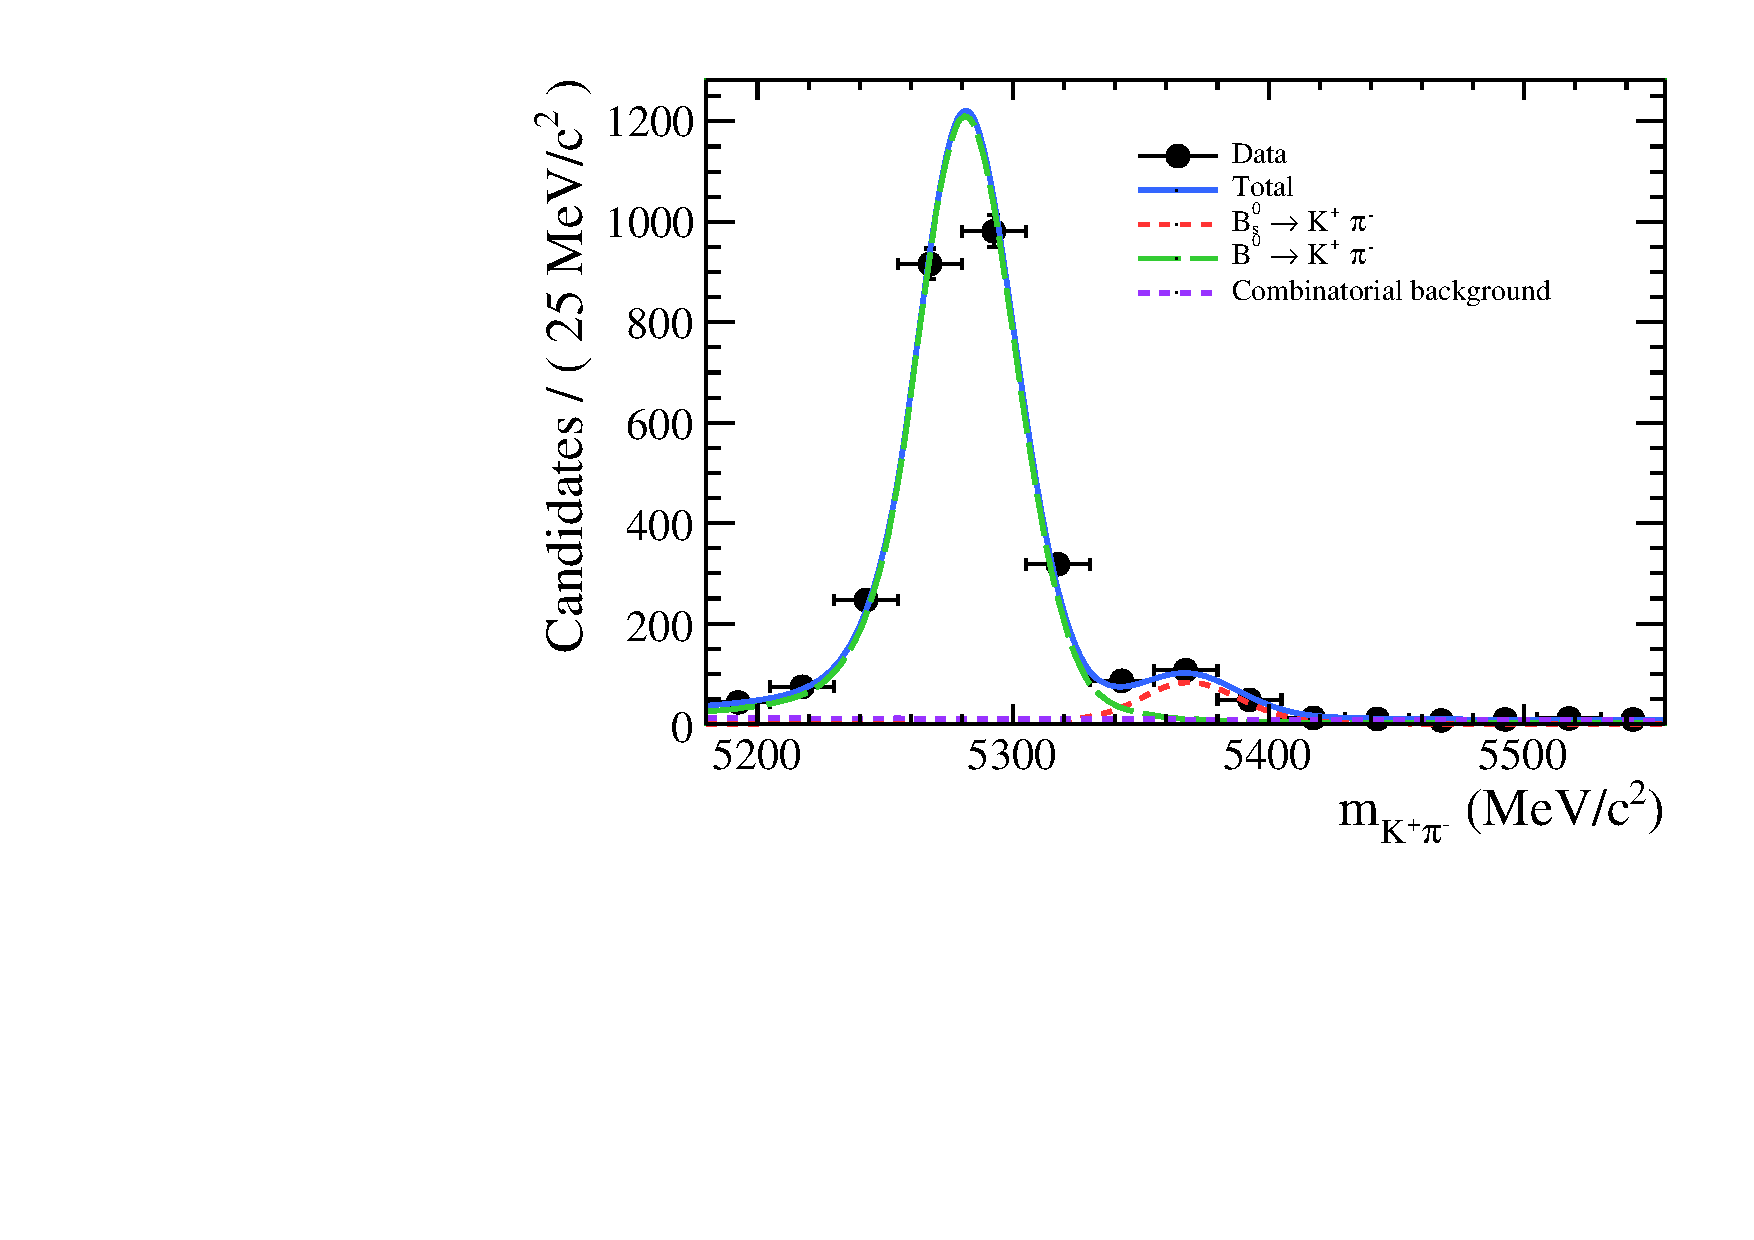
\includegraphics[width=0.6\textwidth]{./Figs/LifetimeSystematics/Bd2KPi_mass_fit.pdf}
\caption{Maximum likelihood fit to the mass distribution of \bdkpi decays for data taken in 2011, 2012, 2015 and 2016. Components for \bdkpi, \bskpi and combinatorial background decays are included in the mass fit. }
\label{fig:bdkpimassfit}
\end{figure}


The decay time \pdf has the same form as the one used for the \bsmumu decays in equation~\ref{} and the acceptance parameters are found from a fit to weighted '\bdkpi simulated decays using the same method described in Section~\ref{}. In the same way as \bsmumu decays the number of tracks in the event are re-weighted using the same weights as for \bsmumu decays. However the yearly weights applied to combined simulated \bdkpi decays from each year are not dependant on \bsjpsiphi decays. Since \bdkpi decays have a high yield in data, mass fits to each year are used to find the yields and combined the simulated decays from each year. The same mass \pdf used to fit the combined mass distribution is applied to each year. This simplifies the efficiency terms and the weights combining simulated decays in different years are then computed as
\begin{equation}
X = Y
\end{equation}

The acceptance function fit is shown in Figure~\ref{fig:bdkpiacceptancefit}. 

\begin{figure}[htbp]
\centering
  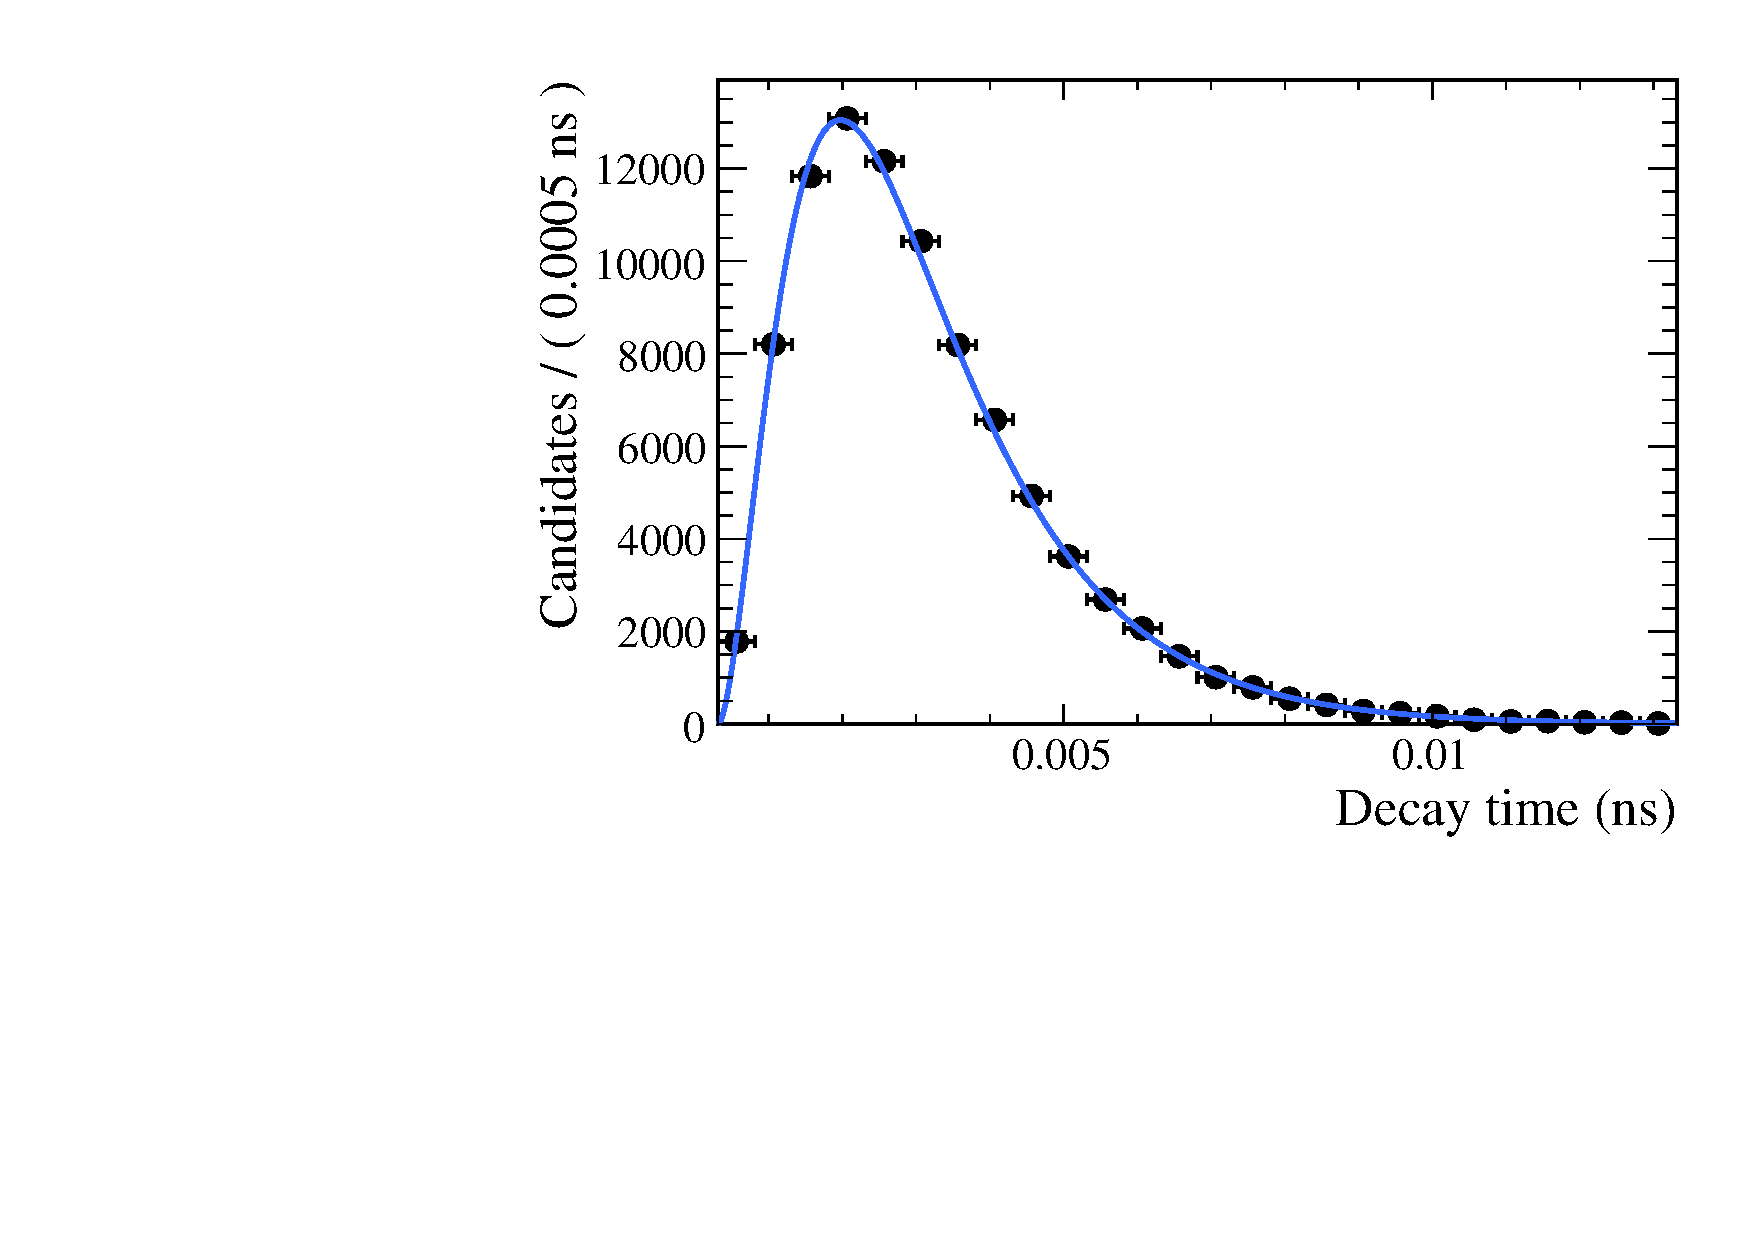
\includegraphics[width=0.6\textwidth]{./Figs/LifetimeSystematics/Bd2KPi_acceptance_fit.pdf}
\caption{Decay time distribution in weighted 2011, 2012, 2015 and 2016 simulated decays and the \ml fit results to determine the acceptance function parameters. }
\label{fig:bdkpiacceptancefit}
\end{figure}

The measured \bdkpi lifetime and inverse lifetime are
\begin{equation}
\tau_{K\pi} = 1.52 \pm 0.03  \text{ ps} 
\end{equation}
%%\begin{equation}
%\Gamma_{K\pi} = XX  \pm XX \text{ ps}^{-1}
%\end{equation}
where only the statistical uncertainty is given and the decay time fit is shown in Figure~\ref{fig:bdkpilifetimefit}. The measured results are consistent with the PDF value of 1.520 $\pm$ 0.004 \ps. Therefore the measurement strategy used to find the \bsmumu \el has been shown to work. The statistical uncertainty of the \bdkpi decay time fits are assigned as systematic uncertainties to provide a measure of how well the acceptance function can be determined from weighted simulated decays for measuring \tmumu and \Gmumu. 

\begin{figure}[htbp]
\centering
  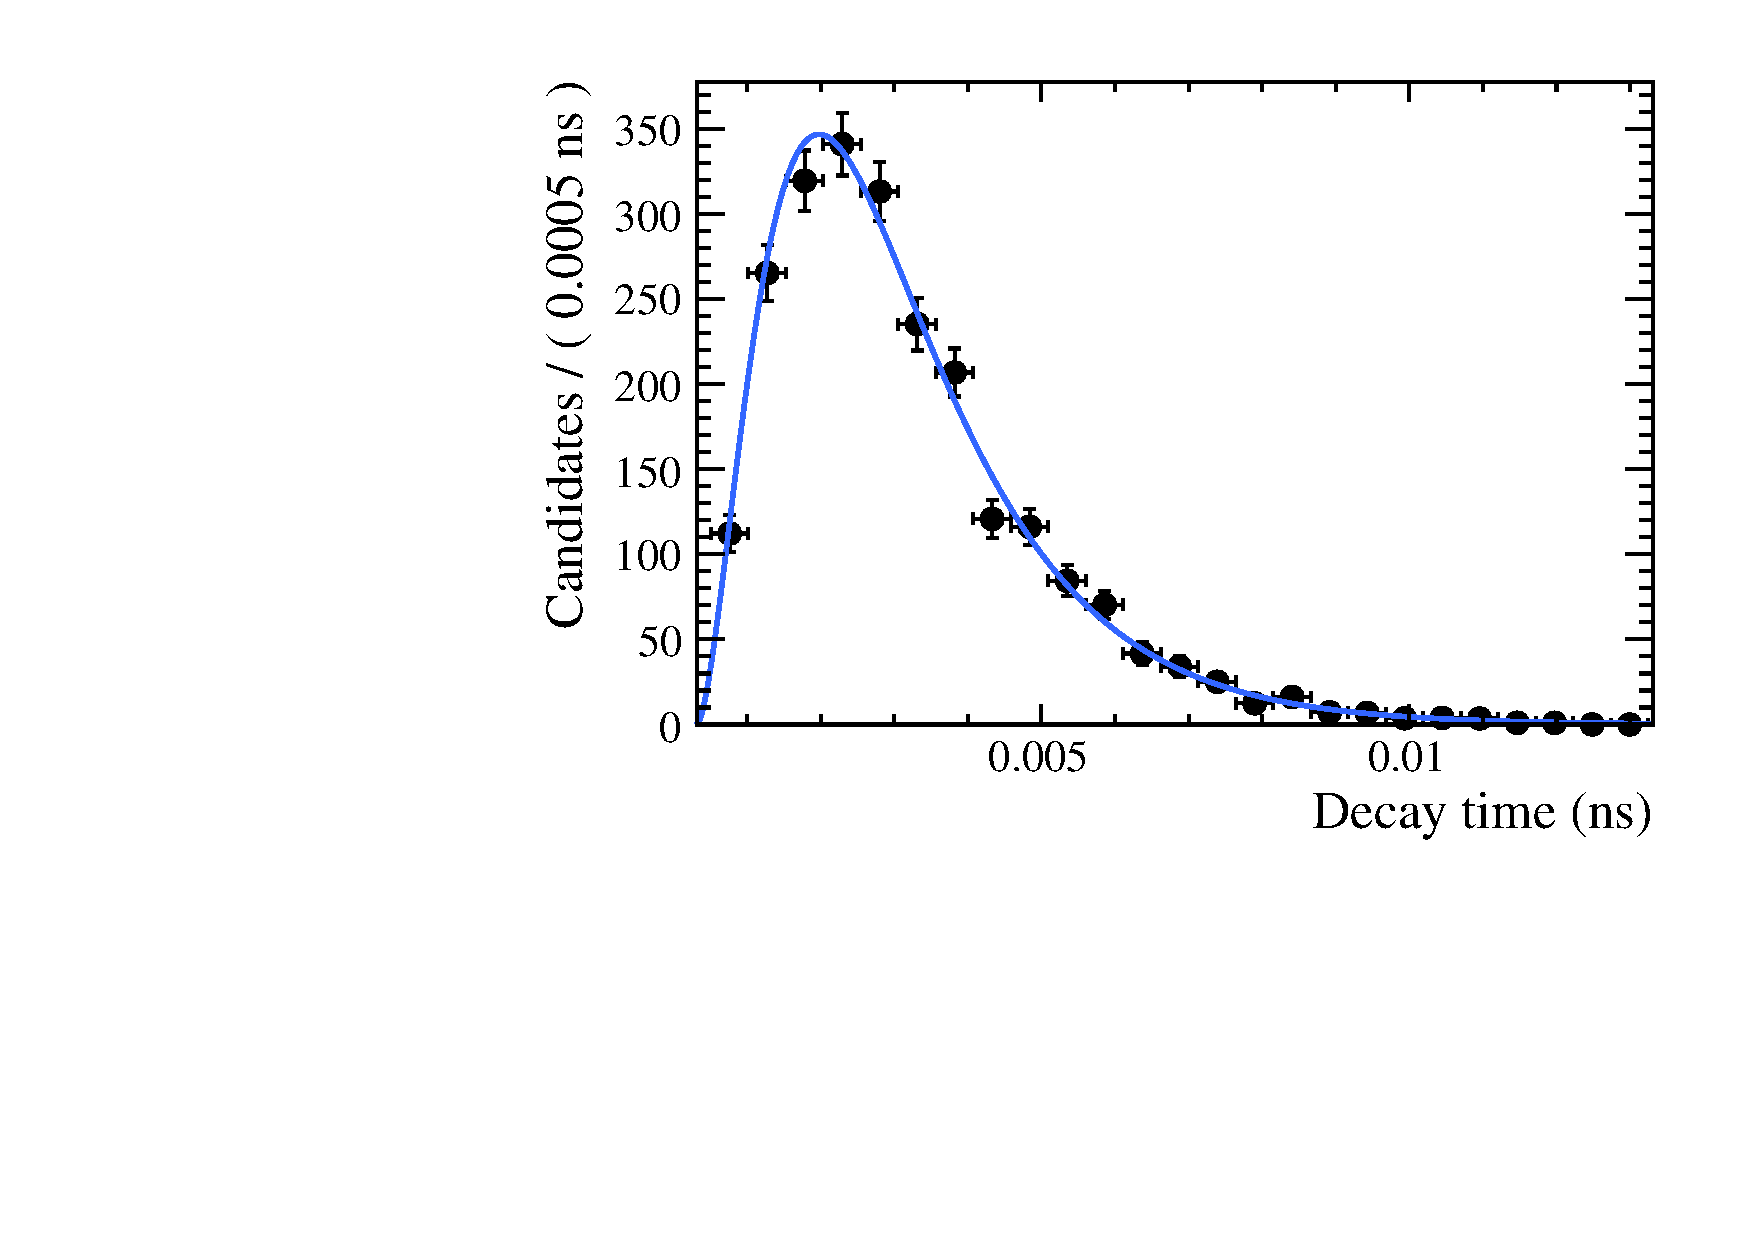
\includegraphics[width=0.6\textwidth]{./Figs/LifetimeSystematics/Bd2KPi_lifetime_fit.pdf}
\caption{Maximum likelihood fit to the signal weighted decay time distribution of \bdkpi decays for data taken in 2011, 2012, 2015 and 2016. }
\label{fig:bdkpilifetimefit}
\end{figure}

However, the determination of the \bsmumu acceptance function relies on weights taken from the number of tracks in an event fro \bdkpi decays in data and simulation. Although the measurement of the \bdkpi lifetime shows the procedure and weighting method works for \bdkpi decays it does not show that the weights taken from \bdkpi decays for the number of tracks in an event can be applied to other decays. Therefore as a cross check, the lifetime of \bskk decays is also measured. 

The same measurement strategy is used for \bskk decays as \bsmumu and \bdkpi and candidates in 2012 and 2015 data are identified using the selection requirements in Chapter~\ref{}. Once again TIS triggers are used to keep a lifetime unbiased trigger efficiency and candidates are reconstructed assuming both daughters are kaons. The mass \pdf includes \bskk and combinatorial background decays only and the same \pdf is used for \bskk as for \bskpi. An unbinned \ml fit used to extract the sWeights is shown in Figure~\ref{fig:bskkmassfit}. 

\begin{figure}[htbp]
\centering
  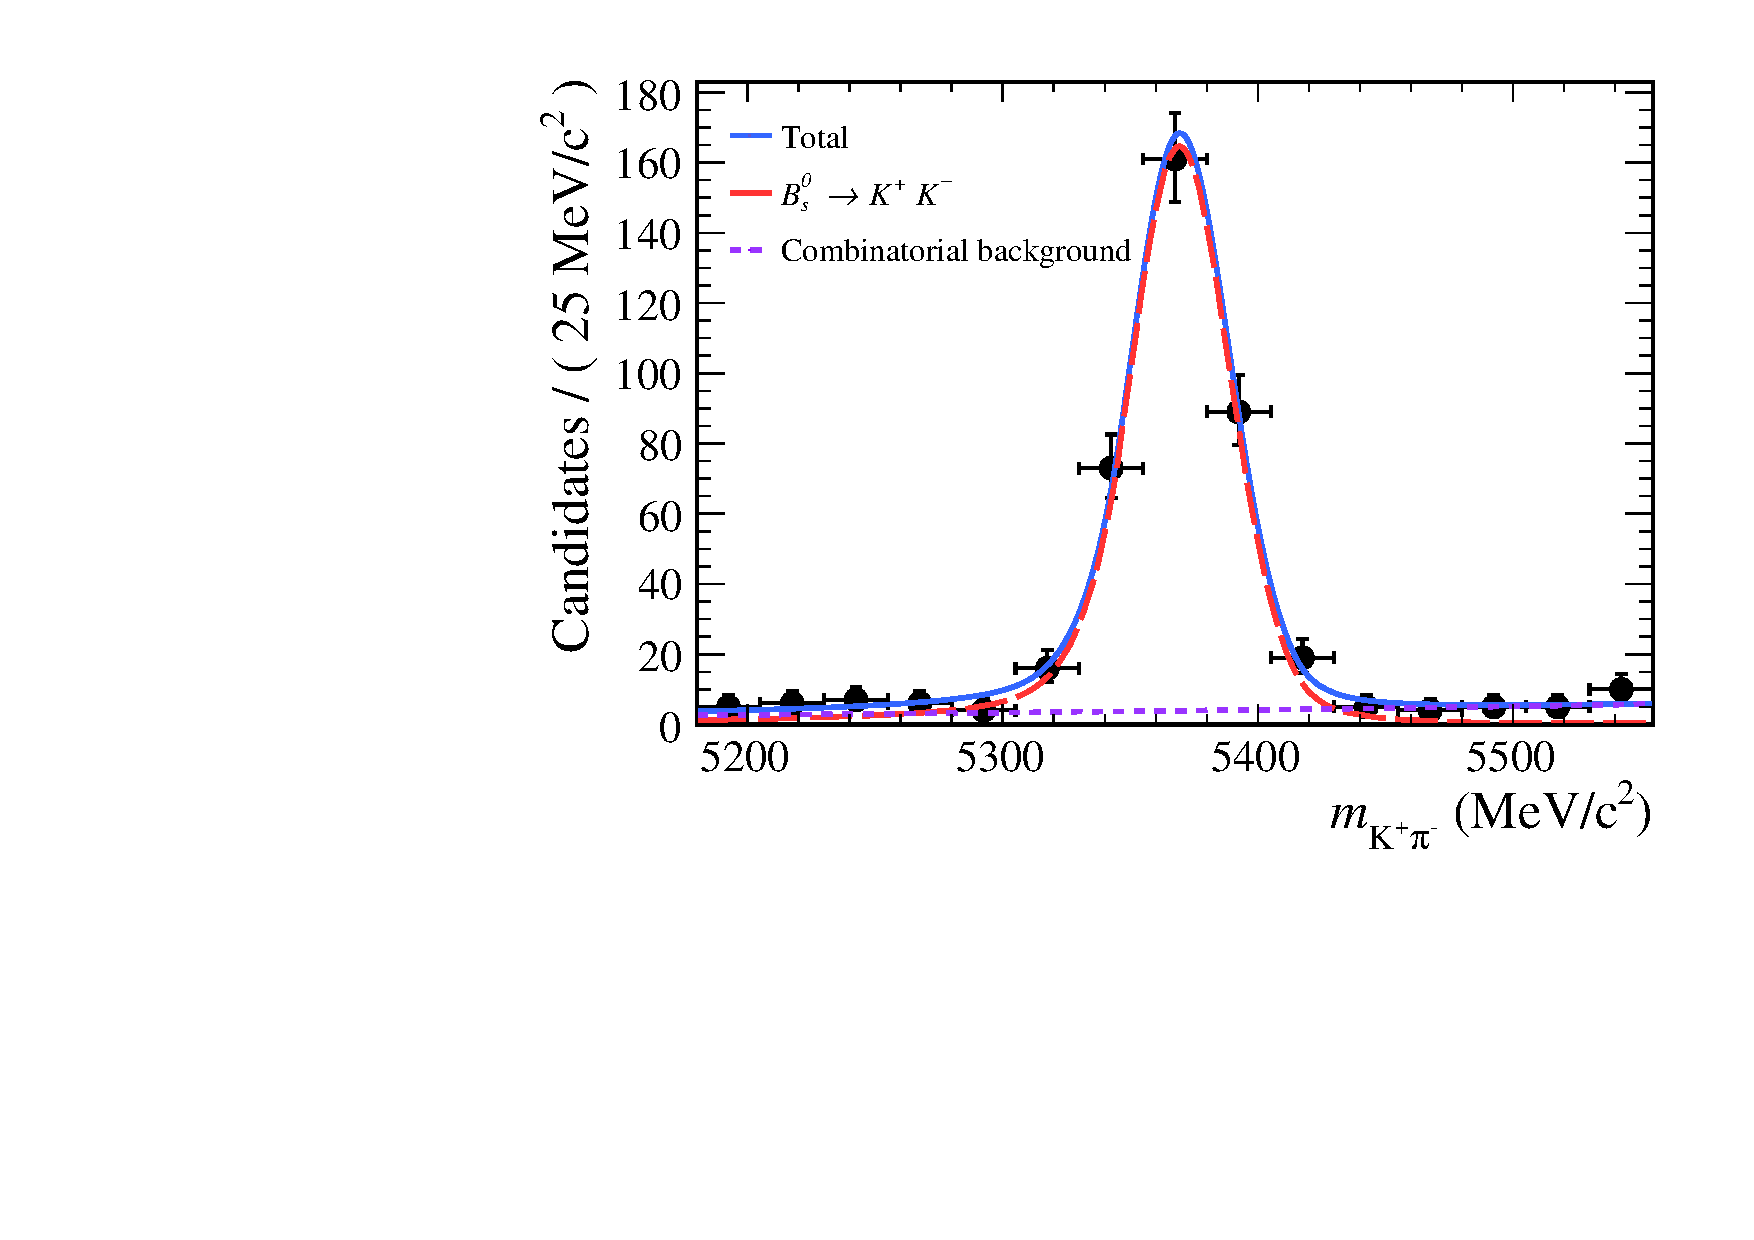
\includegraphics[width=0.6\textwidth]{./Figs/LifetimeSystematics/Bs2KK_mass_fit.pdf}
\caption{Maximum likelihood fit to the mass distribution of \bskk decays for data taken in 2012 and 2015. Components for \bskk and combinatorial background decays are included in the mass fit. }
\label{fig:bskkmassfit}
\end{figure}


The \bskk acceptance is found using the same method as \bsmumu with \bsjpisphi decays used to determine the relative proportions of decays in each year of data. Figure~\ref{fig:bskkacceptancefit} shows the acceptance function fit and the decay time fit to data. The measured values for the lifetime, $\tau_{KK}$ and the inverse lifetime $\Gamma_{KK}$ are
\begin{equation}
\tau_{KK} = 1.39 \pm 0.06  \text{ ps} 
\end{equation}
%\begin{equation}
%\Gamma_{KK} = XX  \pm XX \text{ ps}^{-1}
%\end{equation}
where only the statistical uncertainty is given and the fit results are shown in Figure~\ref{fig:bskklifetimefit}. The measured values are consistent with the predicted value of 1.395 $\pm$ 0.020 \ps \cite{} and therefore shows that \bdkpi weights can be used for other decays as well as \bdkpi. 

\begin{figure}[htbp]
\centering
  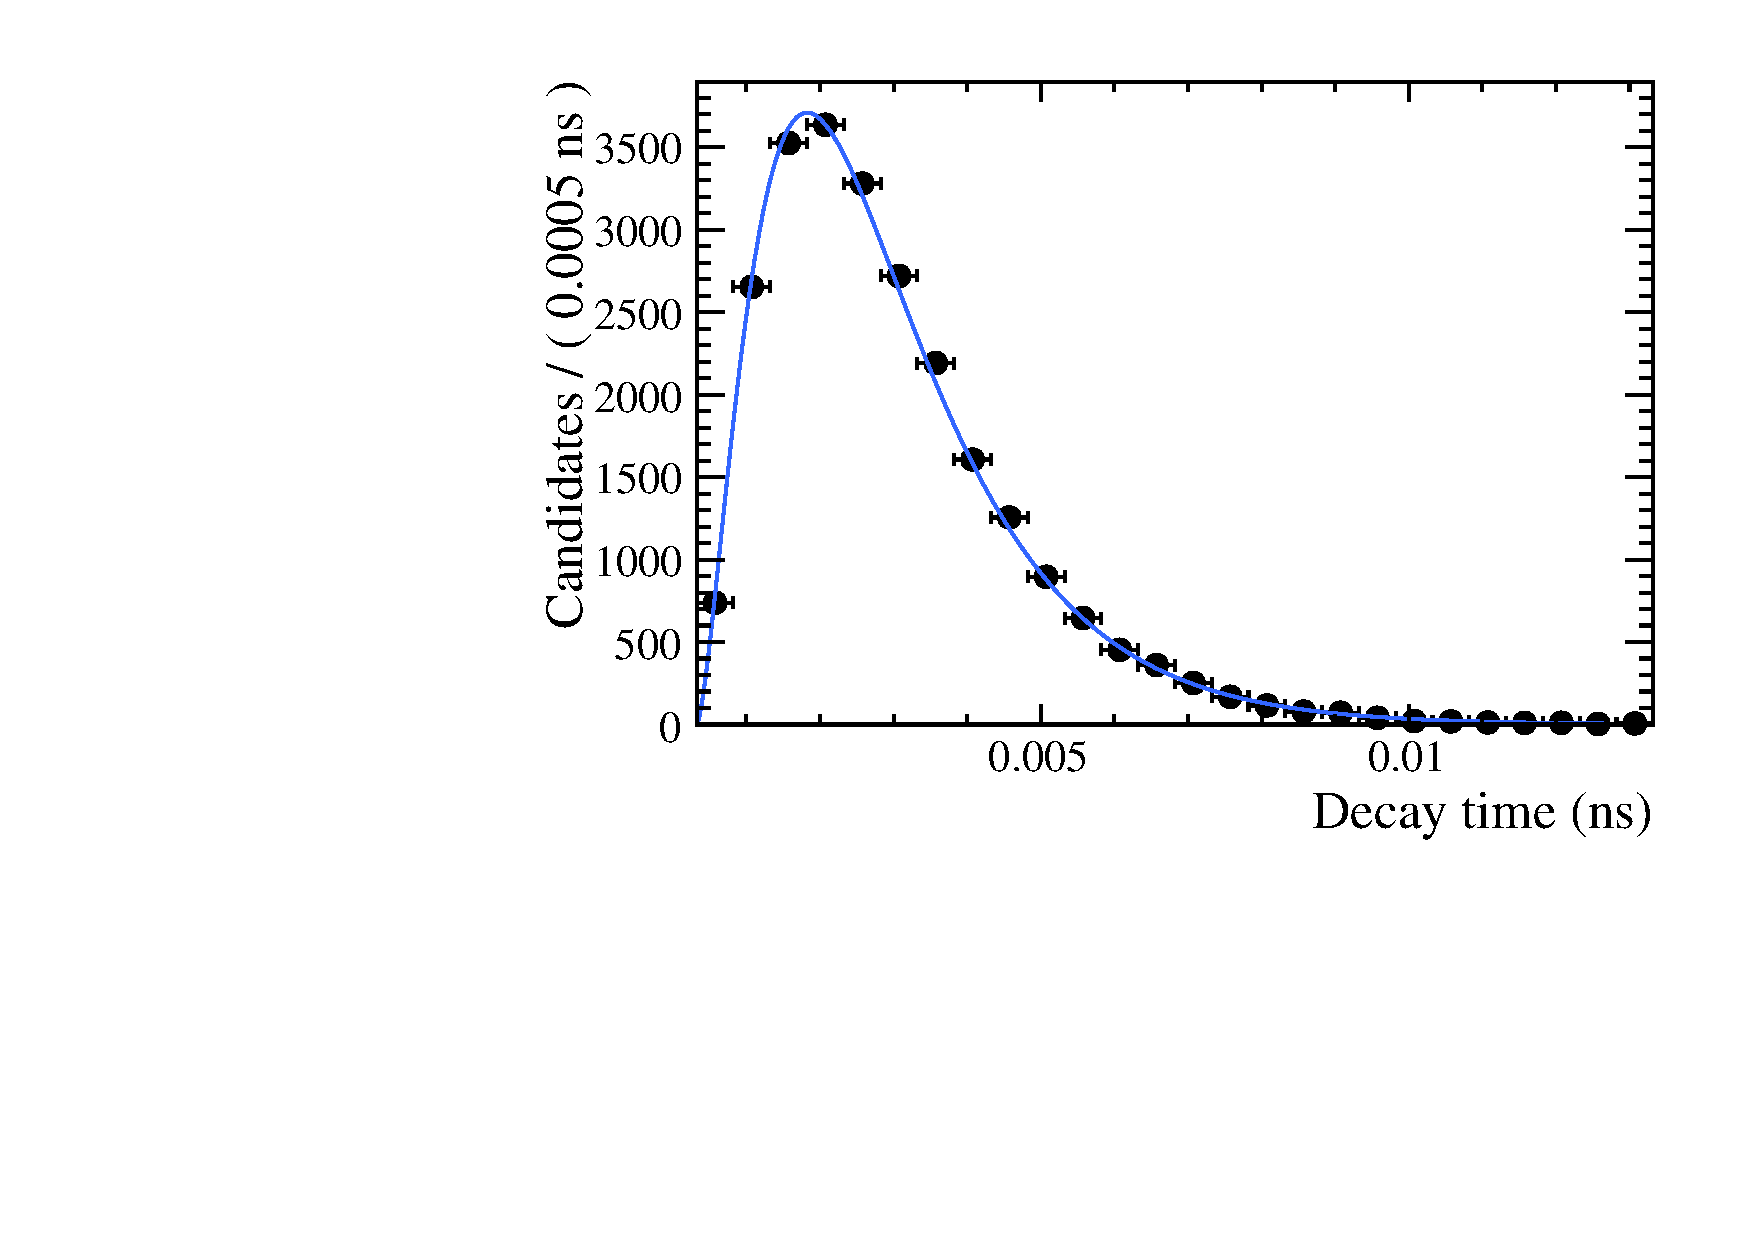
\includegraphics[width=0.6\textwidth]{./Figs/LifetimeSystematics/Bs2KK_acceptance_Fit.pdf}
\caption{Decay time distribution in weighted 2012 and 2015 simulated decays and the \ml fit results to determine the acceptance function parameters. }
\label{fig:bskkacceptancefit}
\end{figure}

\begin{figure}[htbp]
\centering
  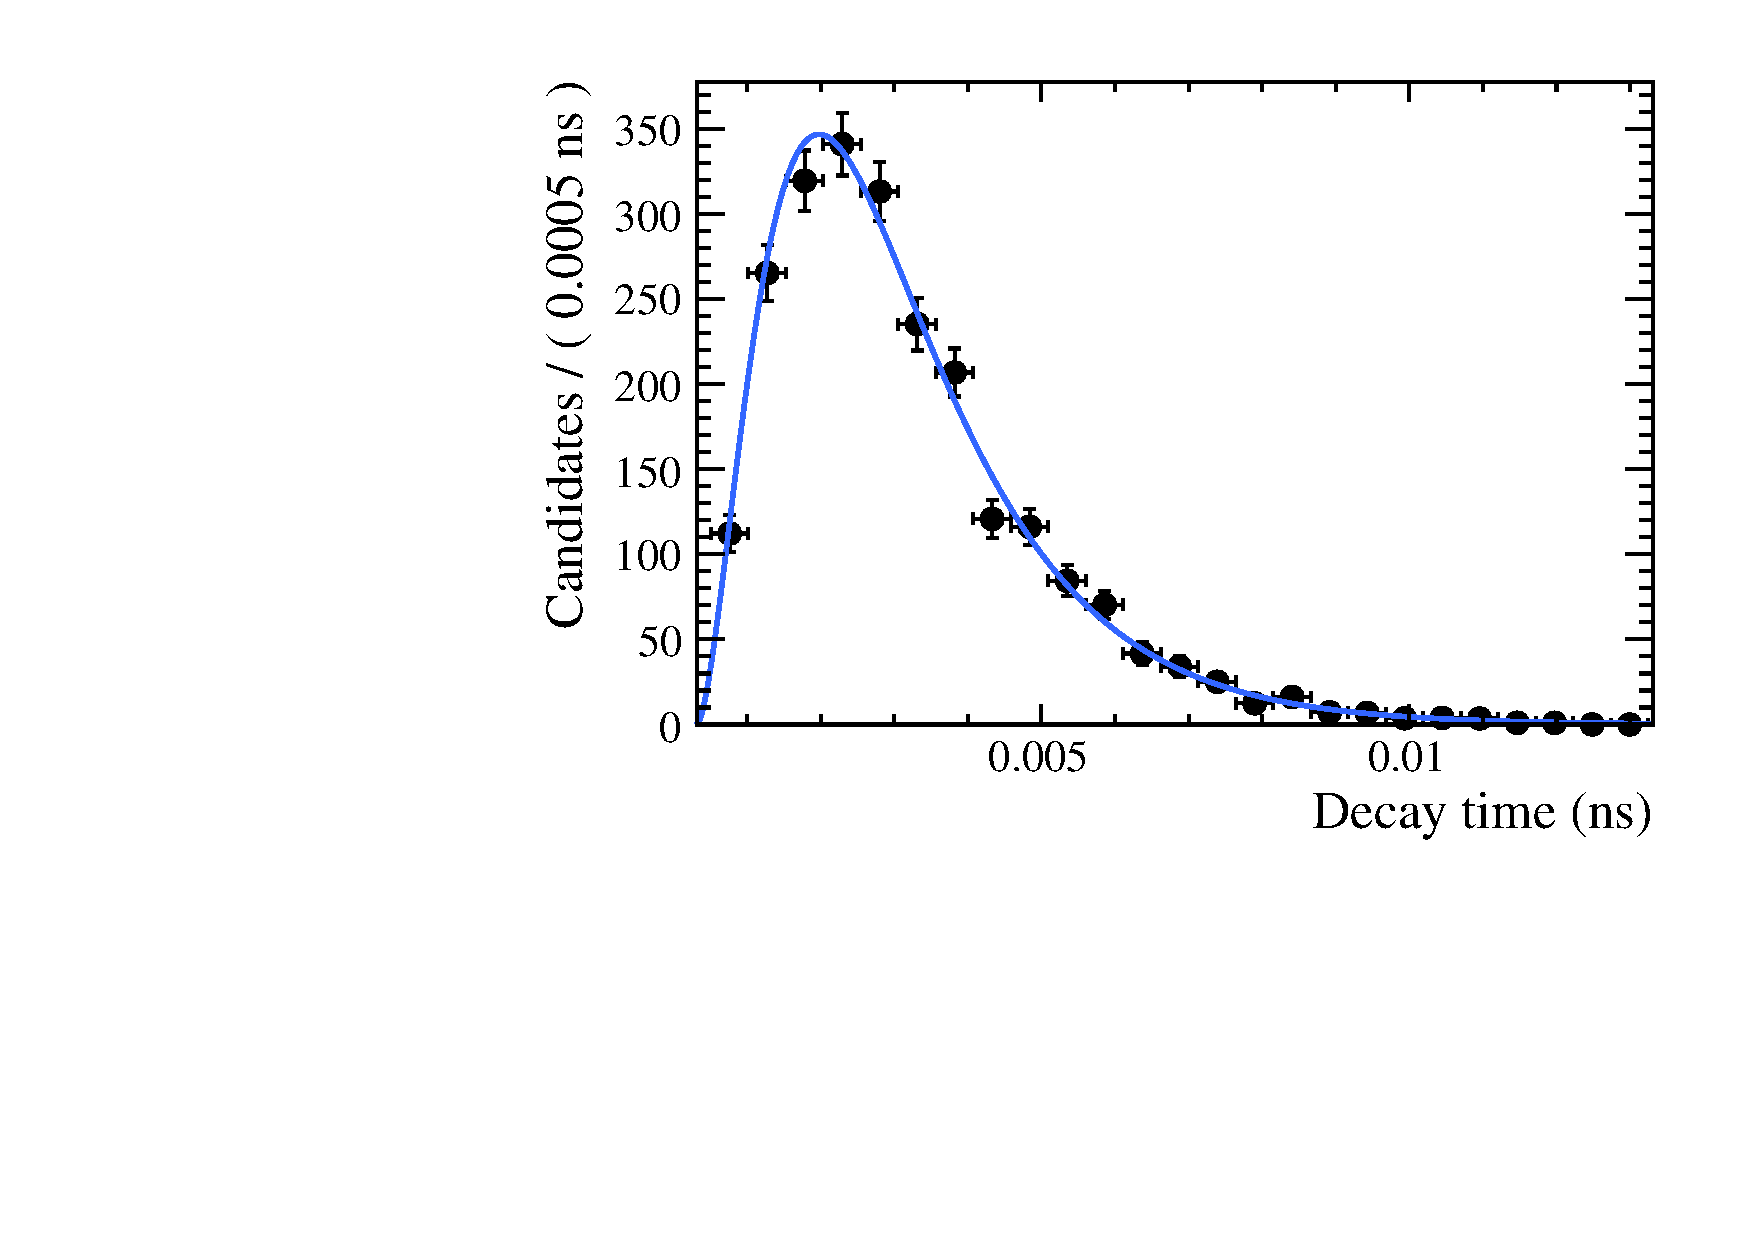
\includegraphics[width=0.6\textwidth]{./Figs/LifetimeSystematics/Bd2KPi_lifetime_fit.pdf}
\caption{Maximum likelihood fit to the signal weighted decay time distribution of \bskk decays for data taken in  2012 and 2015. }
\label{fig:bskklifetimefit}
\end{figure}

\section{Incorrectly assigned primary vertices and additional detector resolution effects}
\label{sec:PVcheck}
Measuring the \bsmumu effective lifetime accurately relies on the $B^{0}_{s}$ candidate being assigned to the correct primary vertex in the event, incorrect assignment would lead to the wrong value for the decay time of an event
In the papers \cite{Aaij:2016ohx,Aaij:2015vza} that study the lifetime of $B \to J/\psi X$ decays a component is included into the decay time fit to model the number of incorrectly assigned primary vertices (PVs). The decay time fit consists of a \pdf describing X convoluted by the sum of three Gaussian functions; two narrow Gaussian functions model the decay time resolution of the detector and a third wider Gaussian function corresponds to $<1\%$ of decays assigned incorrect PVs. The decay time fit to measure the \bsmumu \el does not explicitly model incorrectly assigned PVs or the detector resolution, however these effects will to some degree be included into the acceptance function. 

A similar model is the papers \citeP{ is used to check the affect of decays with incorrectly assigned PVs and detector resolution effects that are not included in the acceptance function on the measured lifetime. 

The weighted \bsmumu simulated decays used to compute the acceptance function parameters is used to determine the decay time resolution due to the detector resolution and incorrectly assigned PVs. The difference between the reconstructed decay time and the `true' decay time with which decays were generated is computed for each decay that pass the full selection, the resulting distribution is fitted with the resolution function composed of the sum of three Gaussian. The Gaussian have the same mean value, which is left free in the fit along with the widths and fraction of each Gaussian entering. The fit parameters are shown in Table \ref{tab:resolutionfit}.% and the total fit in Figure \ref{fig:resolution_fit_plot}. 
The fit results have a similar form to those used in \cite{Aaij:2016ohx,Aaij:2015vza}, where the detector resolution is modelled with two narrow Gaussian and the Gaussian for incorrectly assigned PVs is broader and describes a small fraction of events.

\begin{table}[ht]
\begin{center}
\begin{tabular}{|l|l|}
\hline
Parameter               & Fit value             \\ \hline
$\mu$ (ps)              & 0.00063 $\pm$ 0.00005 \\ \hline
$\sigma_{1} (ps)$       & 5.62$\pm$0.07         \\ 
$f_{1}$                 & 0.006               \\ \hline
$\sigma_{2} (ps)$       & 0.0573$\pm$ 0.0003    \\ 
$f_{2}$                 & 0.313                \\ \hline
$\sigma_{3} (ps)$       & 0.0294 $\pm$ 0.0001   \\ 
$f_{3}$                 & 0.681                \\ \hline


\end{tabular}
\caption{Parameters from fit to the difference between the reconstructed decay time and the true decay time of each event that passes the full selection for \bsmumu MC. The mean used for all Gaussian is is $\mu$ and $\sigma_{i}$ are the widths of each Gaussian which make up a fraction $f_{i}$ for the total sum.}
\label{tab:resolutionfit}
\end{center}
\end{table}

%\begin{figure}[htbp]
%\centering
%  
\includegraphics[width=0.49\textwidth]{./Figs/placeholder.jpeg}
%\caption{Fit of the sum of 3 Gaussian functions with a common mean to the difference between the reconstructed %decay time and the true decay time of each event that passes the full selection for \bsmumu MC. }
%\label{fig:resolution_fit_plot}
%\end{figure}

The following model is used to generate 1 million events
\begin{equation}
\epsilon (t) [\mathcal{R}(t) \otimes e^{-t/\tau}]
\end{equation}
where $\epsilon (t)$ is the acceptance function with parameters given in Table \ref{} and $\mathcal{R}(t)$ is the resolution function. Decays are generated assuming the \bsmumu effective lifetime is equal to the lifetime of the heavy $B^{0}_{s}$ mass eigenstate. A fit to the generated events is performed to extract the lifetime, in this fit the resolution is not included and only the acceptance function and the exponential for the lifetime. The results from the fit are $\tau\left(\Bs\right) = 1.6098\pm 0.0014 \ps$, which is consistent with the lifetime of generate events. The difference between the lifetime used to generate events and the fitted value is 0.0002 ps, a factor of 10 smaller than the lowest systematic uncertainty. This cross check shows that the presence of incorrectly assigned PVs or detector resolution effects that are not included in the acceptance function have a negligible effect on the \bsmumu effective lifetime.


 We assume that MC gives good estimate of the number of incorrectly assigned PVs, as a check Figure \ref{fig:Bd2KPi_nPVs_MC_data_comparison} shows the number of \bdkpi events passing the selection outlined in Section \ref{sec:lifetime_sys_acceptance} for MC and sWeighted data for each year. On average there are more PVs per event in MC compared to data therefore using MC would give an overestimation of the number of incorrectly assigned PVs expected in data. 

\begin{figure}[htbp]
  \centering
    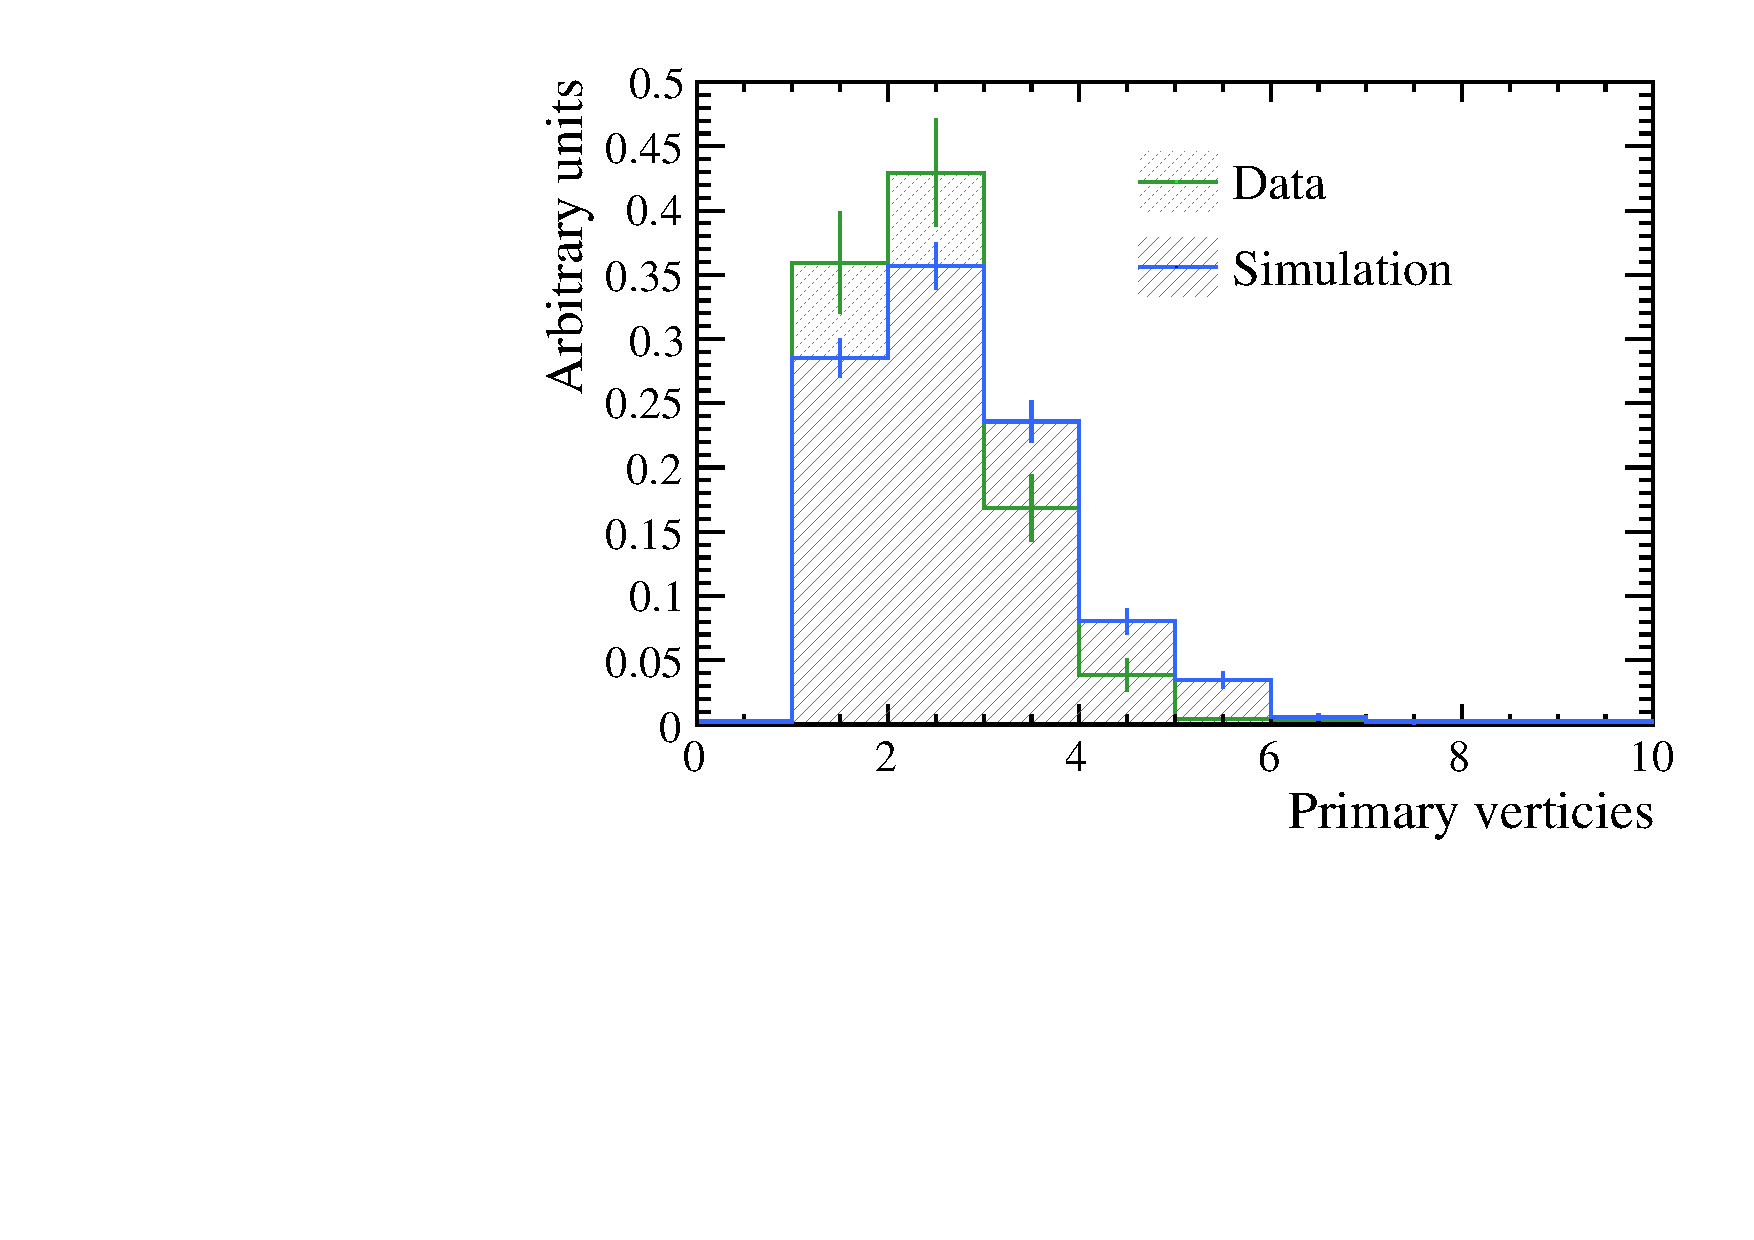
\includegraphics[width=0.49\textwidth]{./Figs/LifetimeSystematics/2011_nPVs.pdf}
    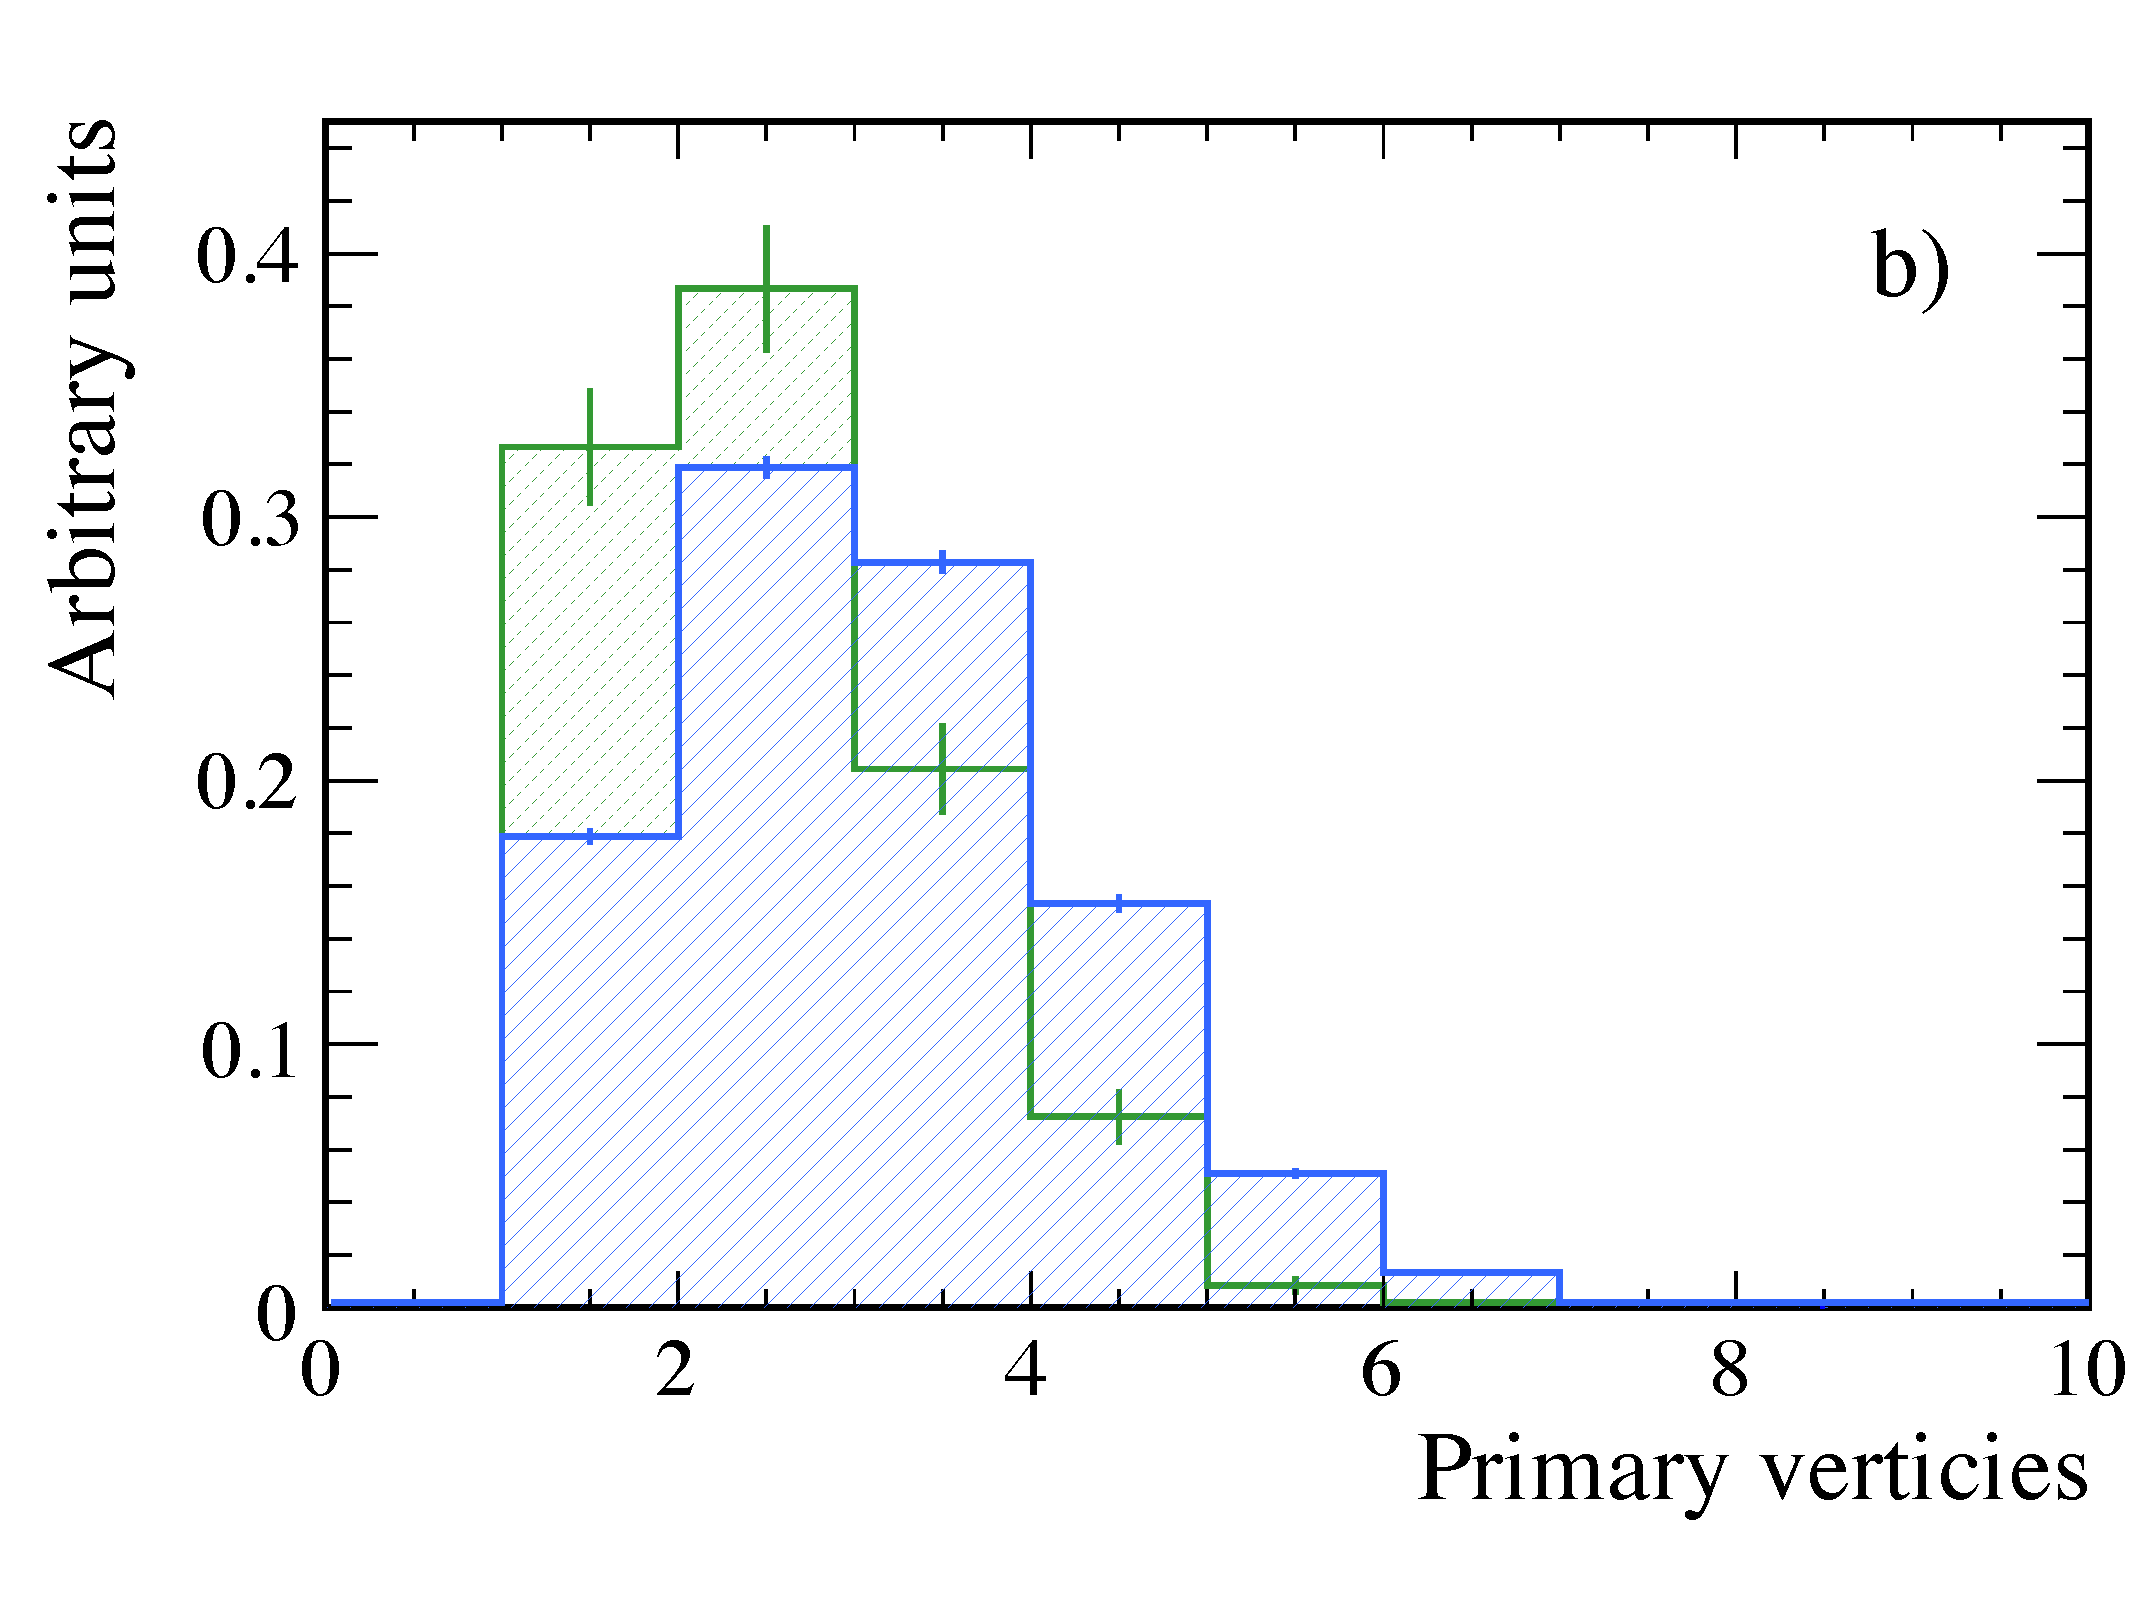
\includegraphics[width=0.49\textwidth]{./Figs/LifetimeSystematics/2012_nPVs.pdf}
    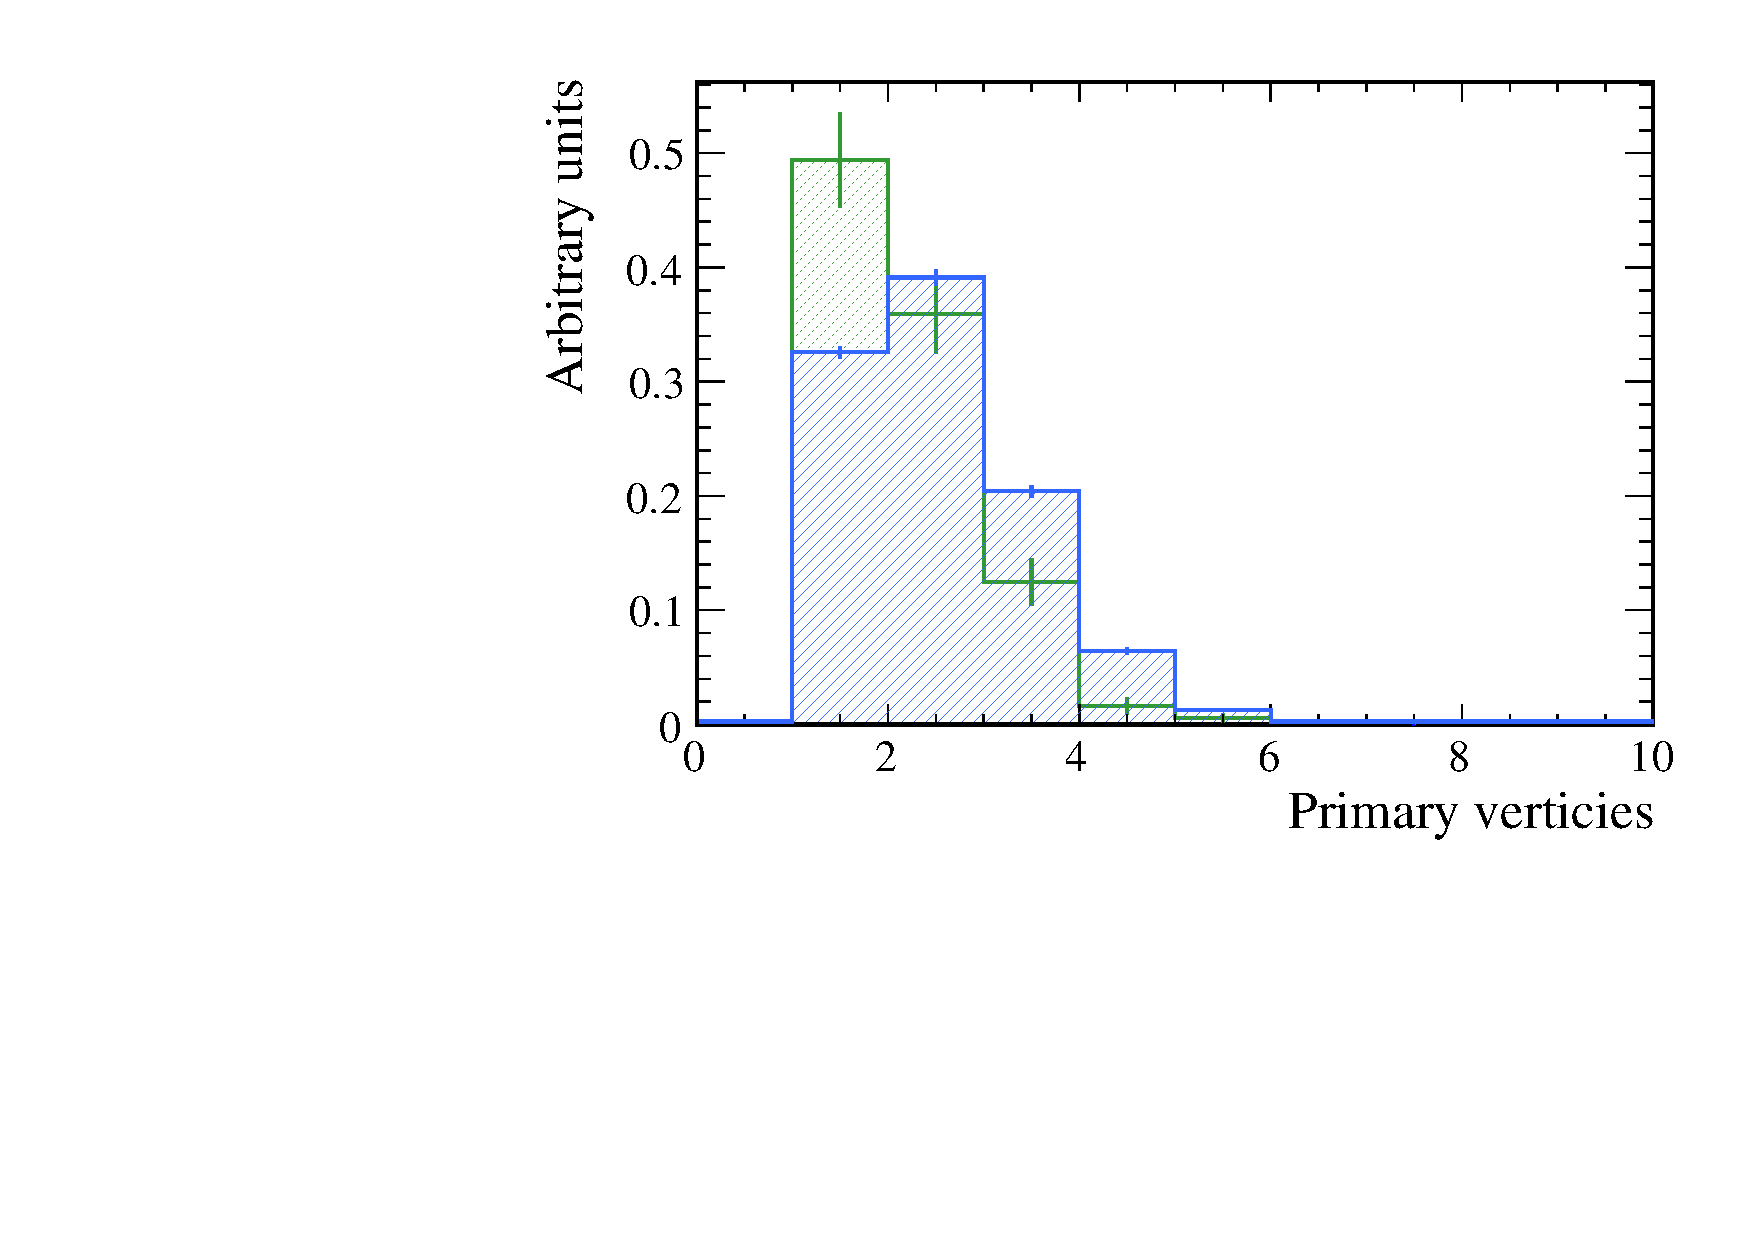
\includegraphics[width=0.49\textwidth]{./Figs/LifetimeSystematics/2015_nPVs.pdf}
    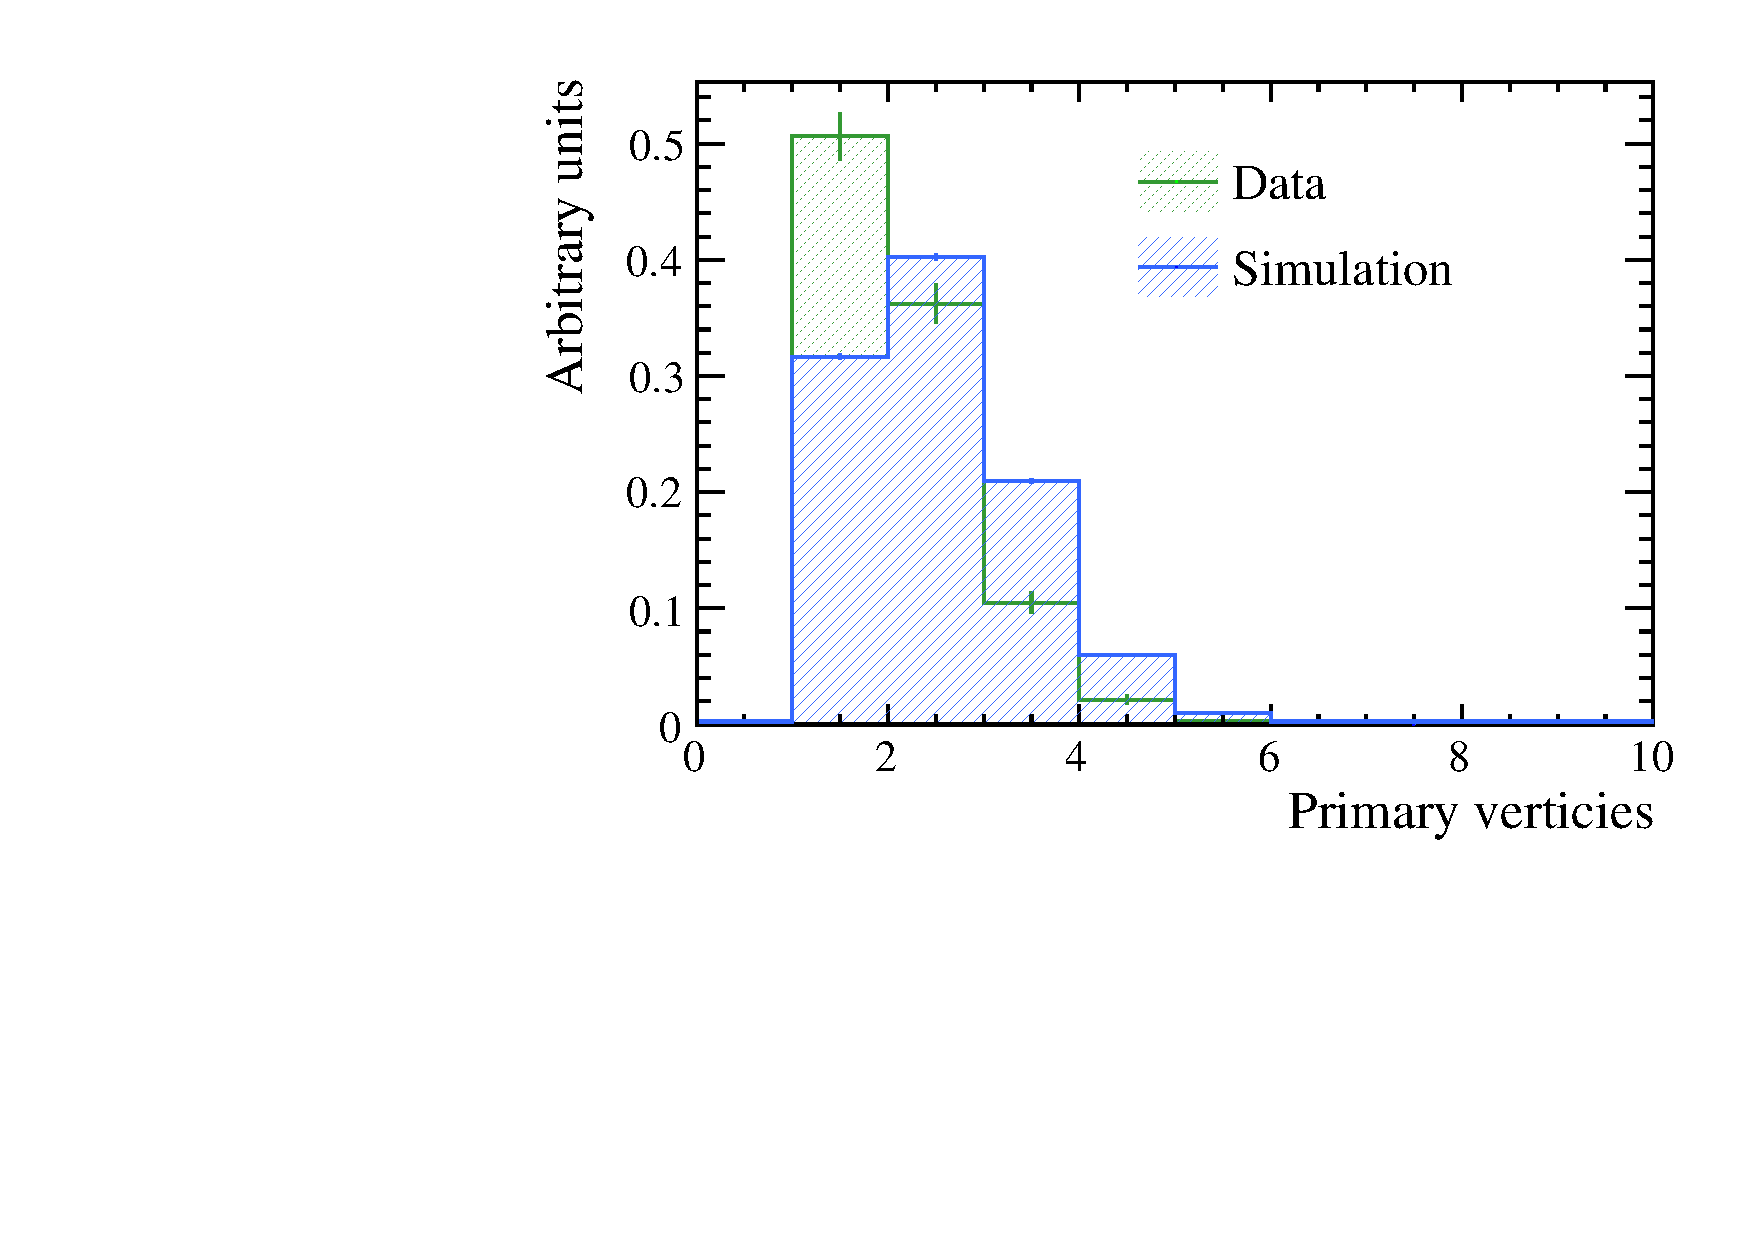
\includegraphics[width=0.49\textwidth]{./Figs/LifetimeSystematics/2016_nPVs.pdf}
  \caption{The distributions for the number of primary vertices in an event \bdkpi data (green triangles) and simulated candidates (blue squares) for 2011 (top left), 2012 (top right), 2015 (bottom left) and 2016 (bottom right), for events that pass the selection in Section \ref{sec:lifetime_sys_acceptance}.}
  \label{fig:Bd2KPi_nPVs_MC_data_comparison}
\end{figure}


\section{Combinatorial background decay time model}
\label{sec:CBGdecytimemodel}

The decay time distribution of combinatorial background decays is largely unknown due to the nature of the background, the model used for this distribution in the toy studies is described in Section~\ref{}. The decay time distribution of combinatorial background decays consists of mostly a short lived component with a lifetime of X \ps and a long lived conpoment with a lifetime of Y \ps.

The sWeighting method is sensitive to the background decay time components that are significantly longer lived than the signal lifetimes and can lead to biased estimated of \tmumu and \Gmumu. 
During the selection an upper decay time cut is applied to remove long-lived backgrounds, this cut is very effective at stopping the bias entering the final results. However the remaining effect must be evaluated.

As discussed in Section~\ref{} determining the decay time distribution of combinatorial background decays is challenging because there are too few decays left in either \bsmumu decay or \bbbarmumx simulated decays after the selection requirements to determine the decay time \pdf. Therefore the combinatorial background of \bhh decays in the mass range 5600 - 6000 \mevcc is used. The validity of used \bhh backgrounds to model \bsmumu combinatorial backgrounds is tested by studying the average lifetime of combinatorial background decays in bins of global BDT The results are shown in Table~\ref{tab:MeanDecayTimeBDTBins}, for decays in data passing the selection requirements for \bsmumu and \bhh decays and in the mass ranges 5447 - 6000 \mevcc and 5600 - 6000 \mevcc, respectively. At low values of the global BDT the average lifetimes are similar and for both \bsmumu and \bhh background the lifetime increases with the output of the global BDT. Overall \bhh combinatorial background decays are longer lived than \bsmumu combinatorial background decays therefore making the \bhh combinatorial background decay time model a conservative estimate for \bsmumu combinatorial background as far as the affect of long lived components in concerned. 
\begin{table}[htbp]
\begin{center}
\begin{tabular}{|l|c|c|c|c|}
\hline
      & \multicolumn{2}{c|}{\bsmumu} & \multicolumn{2}{c|}{\bhh} \\ \hline
BDT & mean decay      & Number of  & mean decay    & Number of \\
bin & time / \ps      & candidates & time / \ps    & candidates \\ \hline 
1 & $1.178 \pm 0.005$ & 50,695 & $1.124 \pm 0.001$ & 964,502 \\
2 & $1.936 \pm 0.098$ &    244 & $2.394 \pm 0.022$ & 8,838 \\
3 & $2.570 \pm 0.327$ &     46 & $2.781 \pm 0.051$ & 2,373 \\
4 & $2.210 \pm 0.361$ &     17 & $3.023 \pm 0.076$ & 1,125 \\
5 & $2.582 \pm 1.103$ &      4 & $3.417 \pm 0.112$ &   655\\
6 & $2.540 \pm 0.390$ &      3 & $3.978 \pm 0.187$ &   313\\
7 & $2.868 \pm 1.048$ &      2 & $4.626 \pm 0.363$ &   109\\
8 & -                 &      0 & $5.706 \pm 0.683$ &    35\\ \hline
\end{tabular}
\caption{The mean decay time of \bsmumu and \bhh candidates in bins of the global BDT output.}
\label{tab:MeanDecayTimeBDTBins}
\end{center}
\end{table}
The model used for the combinatorial background decay time currently introduced no bias into the pull distribution of \Gmumu for toy studies as shown in Figure~\ref{}. However the size of a systematic bias from the choice of the decay time distribution is estimated by two sets of toy studies. The first uses the background decay time distribution in Table~\ref{} and the second set uses the same decay time distribution of expect the lifetime of each component are made longer by 1 standard deviation and the fraction of the long lived component is increase by one standard deviation as well. For both sets of toy studies only combinatorial background and \bsmumu decays are generated and 10,000 studies are performed for each configuration. 

The resulting pull distribution for \Gmumu are shown in Figure~\ref{fig:CBGextreme}}, the difference in the mean value of the distributions for the two studies is negligible and the width changes by 0.008 \ps$^{-1}$ between the two studies. The change in the width is the largest and therefore is taken as the systematic uncertainty, assuming the median expected uncertainties for \Gmumu and \tmumu. Therefore the systematic uncertainties due to the combinatorial background decay time model are X \ps for \tmumu and Y \ps$^{-1}$ for \Gmumu.

\begin{figure}[htbp]
  \centering
    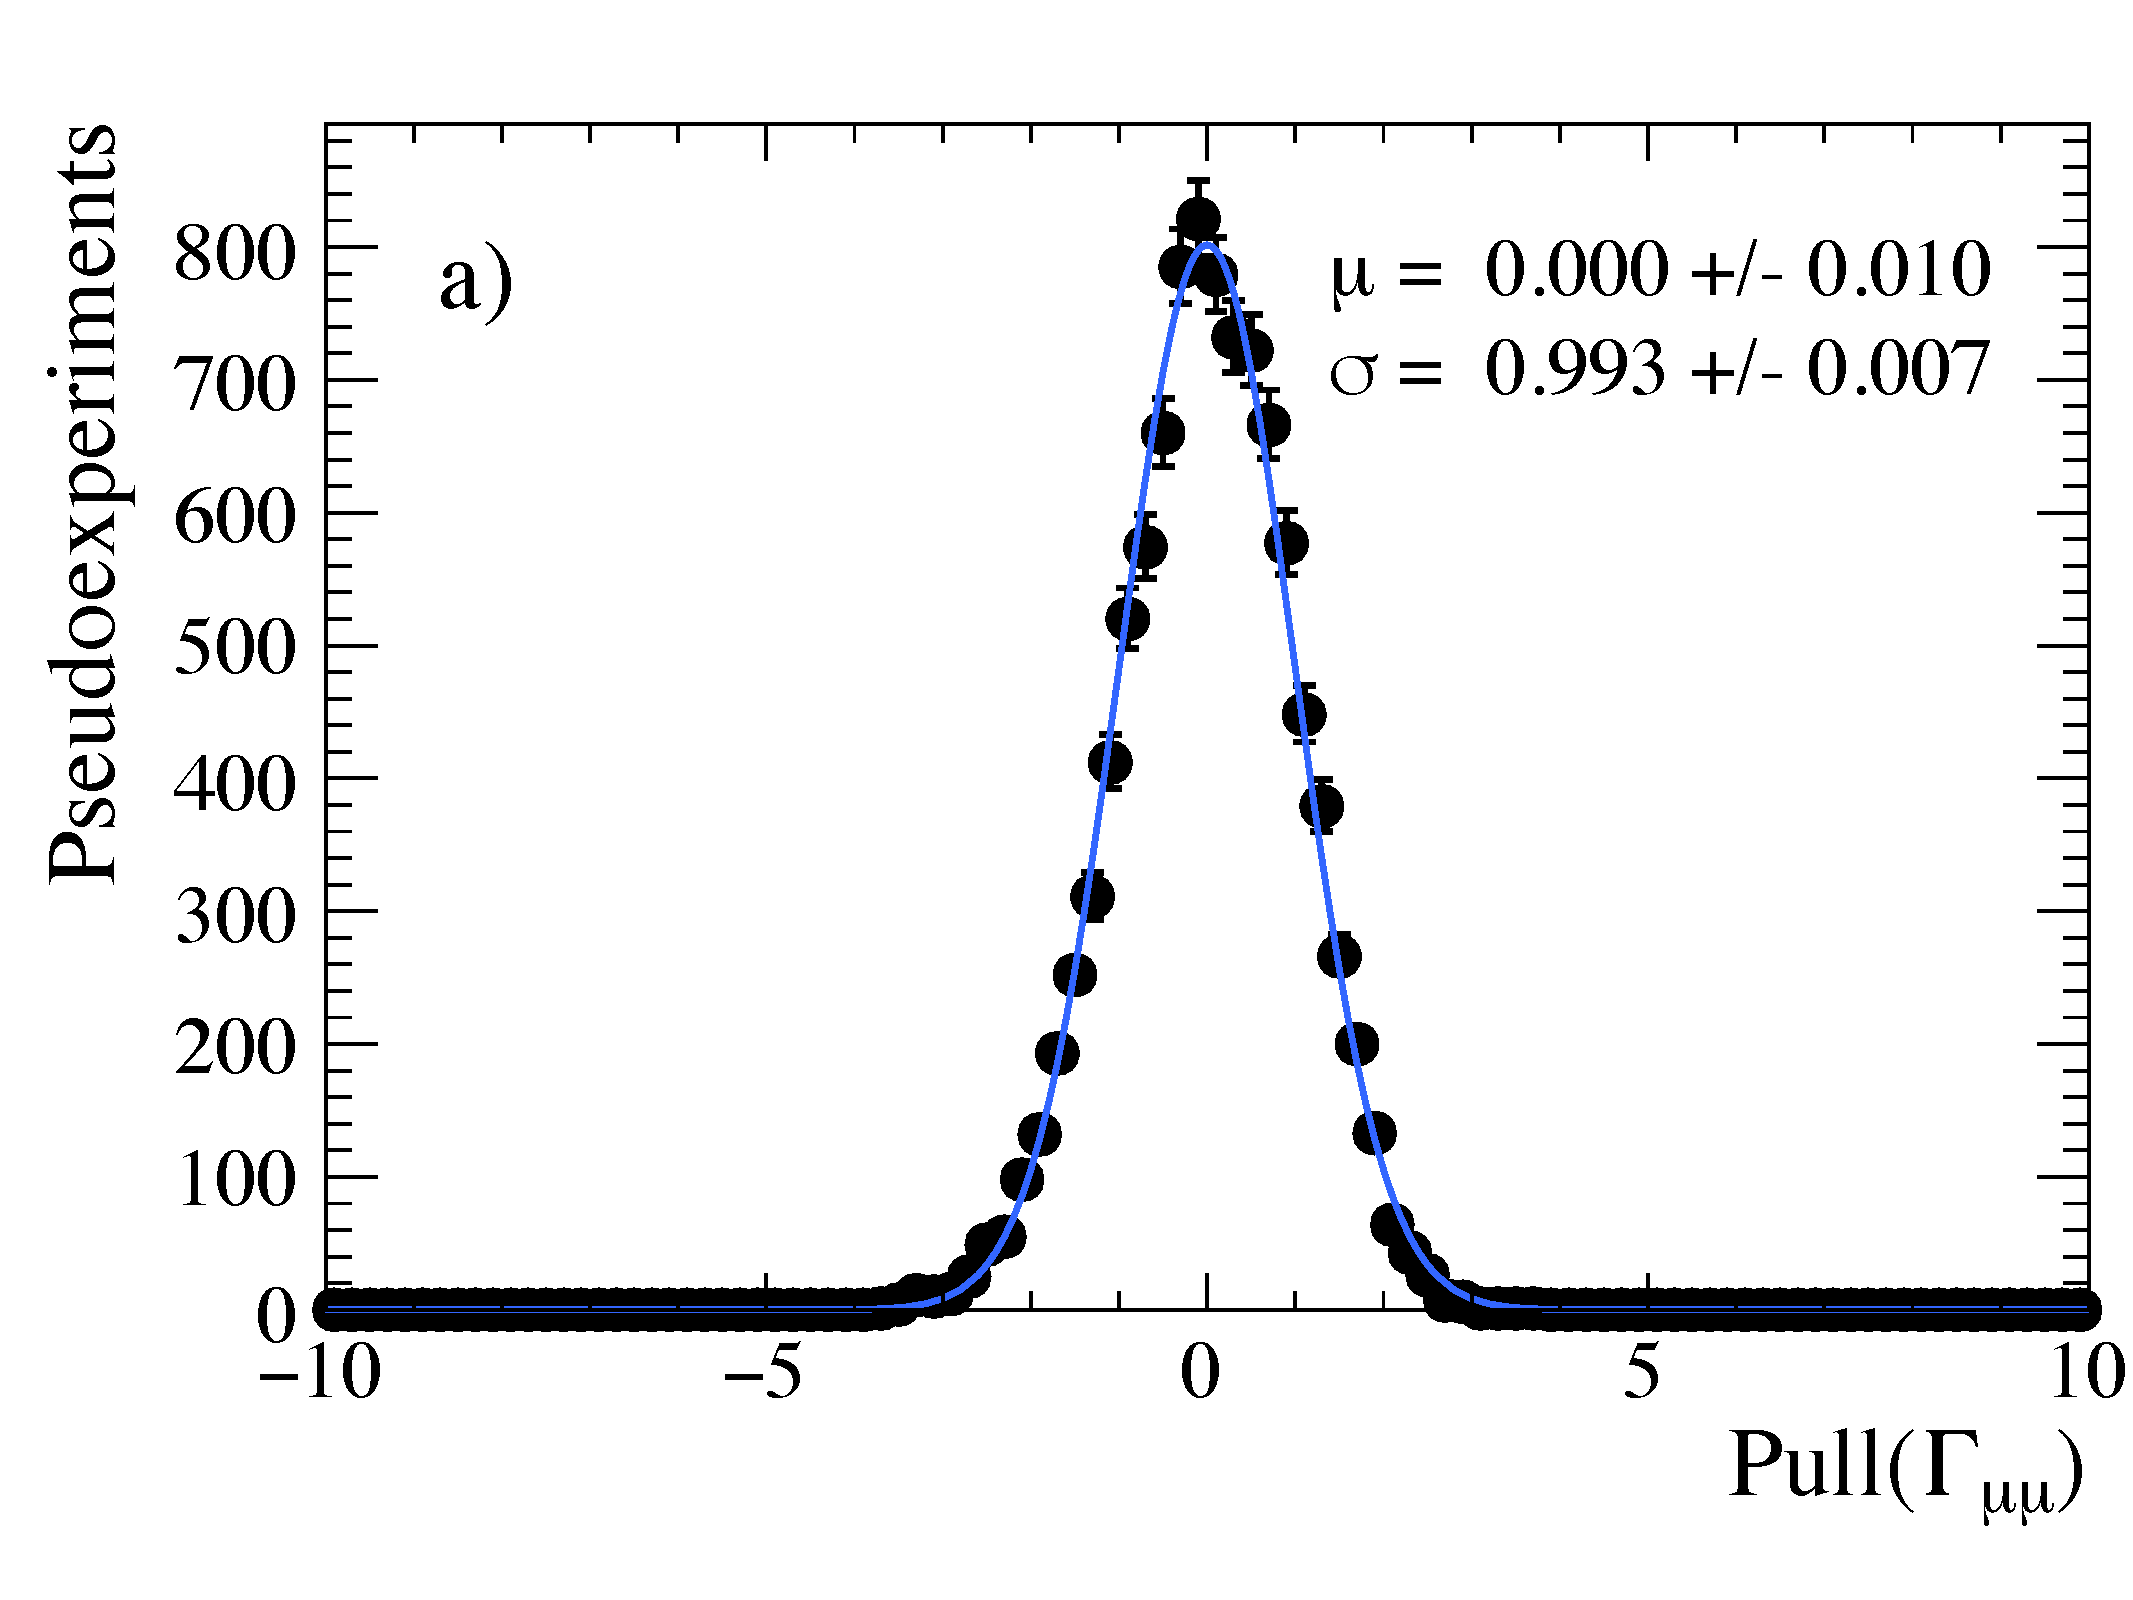
\includegraphics[width=0.49\textwidth]{./Figs/LifetimeSystematics/Gamma_pull_mass_pdf_Run1.pdf}
    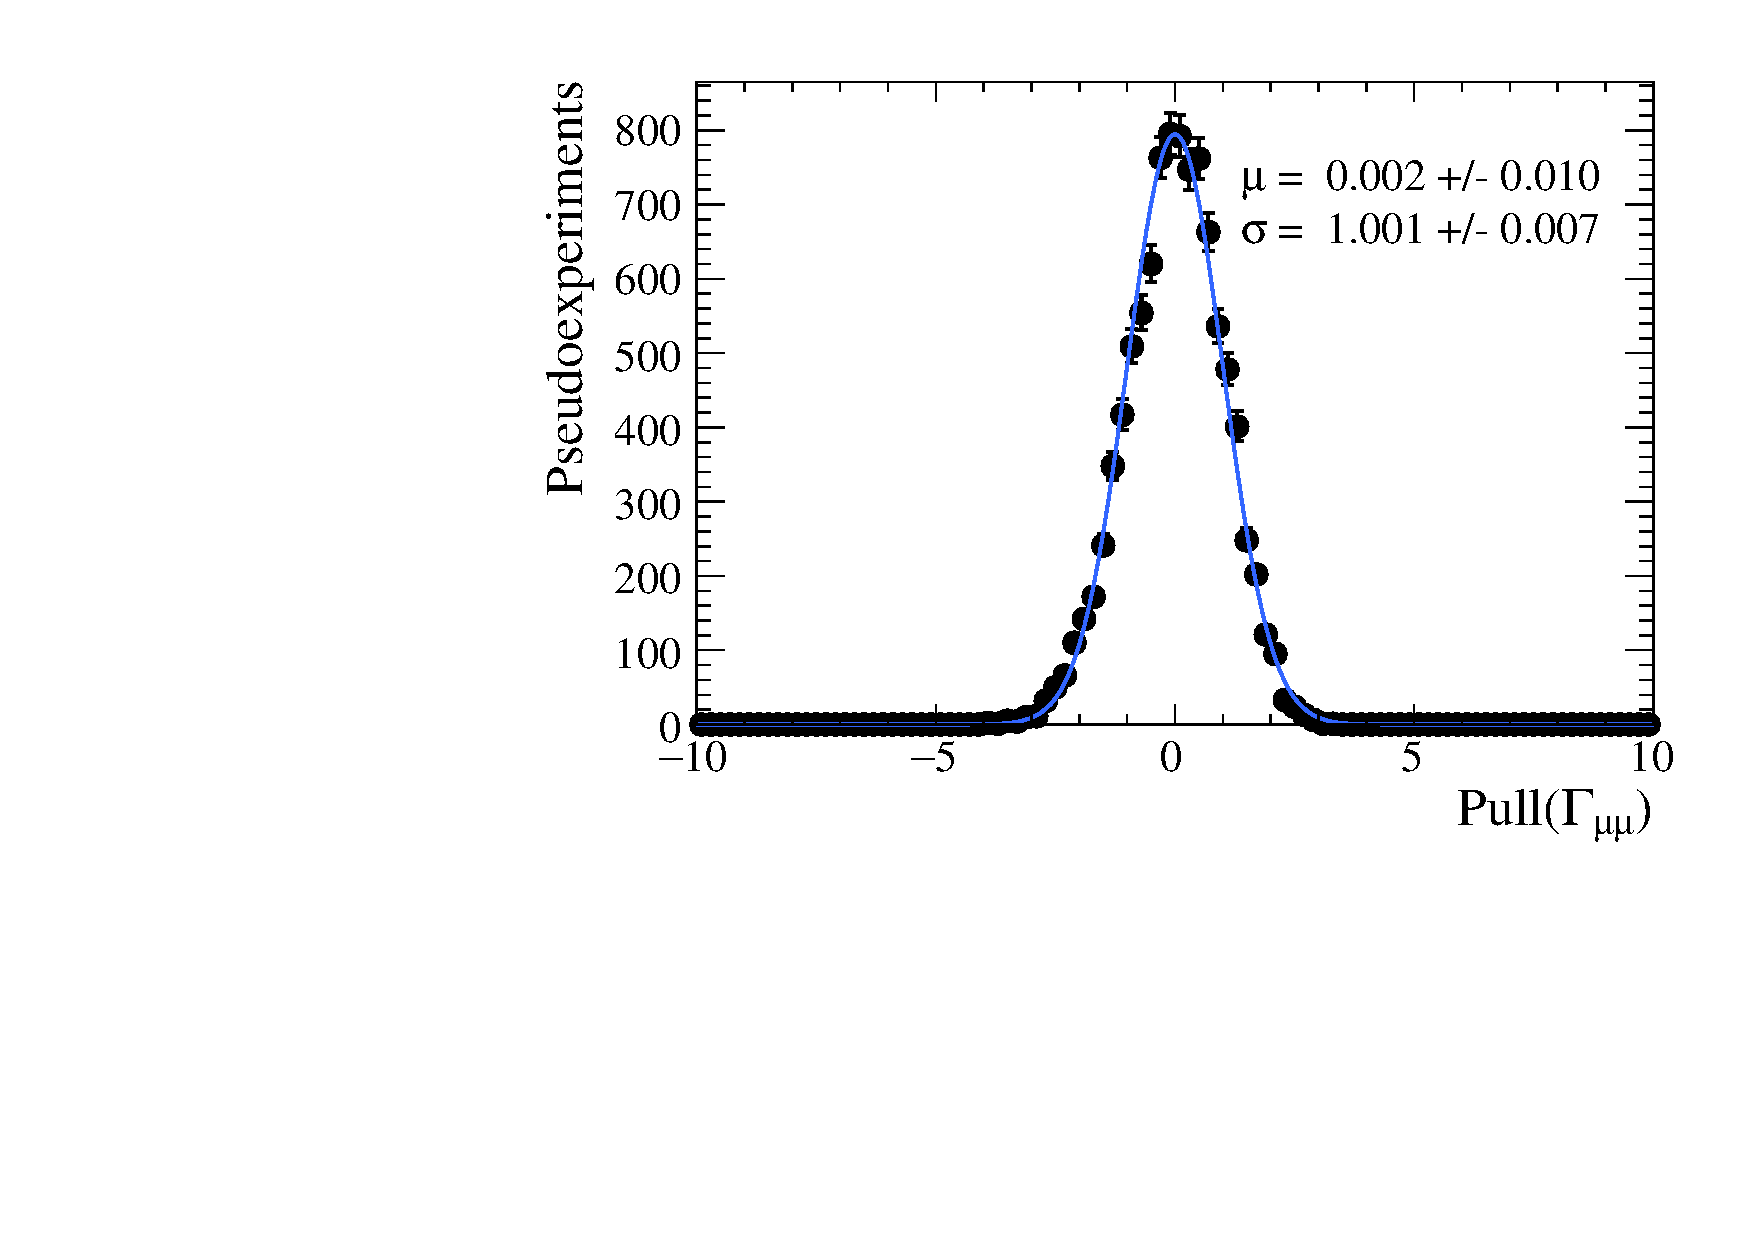
\includegraphics[width=0.49\textwidth]{./Figs/LifetimeSystematics/Bs2MuMu_gamma_pull_CKM_extremeCBG_DT.pdf}

  \caption{.}
  \label{fig:CBGextreme}
\end{figure}


\section{Mix of \bs mass eigenstates}
\label{sec:mixofeigenstates}

In the SM the \bsmumu \el is equal to the lifetime of the heavy \bs mass eigenstate. However the real \bsmumu \el could be between the lifetime of the light and heavy mass eigenstates. %The expected PDG values for the different lifetimes are \tH = and \tL = .

As shown in Section~\ref{} the selection efficiency used to identify \bsmumu decays in data is not uniform across the decay time range. The selection rejects a greater protpotuin of candidates with shown lifetimes compared to candidates with longer lifetimes. Therefore he oresenecce of any \bs light mass eigenstates decaying as \bsmumu in data could be masked by the bias in the decay time distribution. The efficiency to selection light \bs mass eigenstates is lower than the efficiency to select heavy \bs mass eigenstates.

The size of this effect has been estimated using two very simple toy studies. The first assumes that the selection has not bias on the decay time distribution and 1 million candidates are generated with equal contributions from the heavy and light \bs mass eigenstates.% Therefore assuming even missing of the light and heavy mass eigenstates contribution to \bsmumu decays. 
The second set a further 1 million candidates are generate with the same mix of eigenstates but with a more realistic model, using the acceptance function in equation~\ref{} and parameters from Table~\ref{}. The first set of candidates is fitted with a single exponential function and the second set with the acceptance function and exponential function in order to find \tmumu and \Gmumu for each distribution. The acceptance parameters are fixed in the fit.

The values of \tmumu are compared for the two studies and a systematic uncertainty is assigned for the change in \tmumu and values due to the inclusion of the acceptance function. The \ml fits used to measure \tmumu in the two toy studies are shown in Figure~\ref{fig:mixofstates} and the differences between the measured lifetimes for the two studies is 0.018 \ps and is assigned as the systematic uncertainty.

\begin{figure}[htbp]
  \centering
    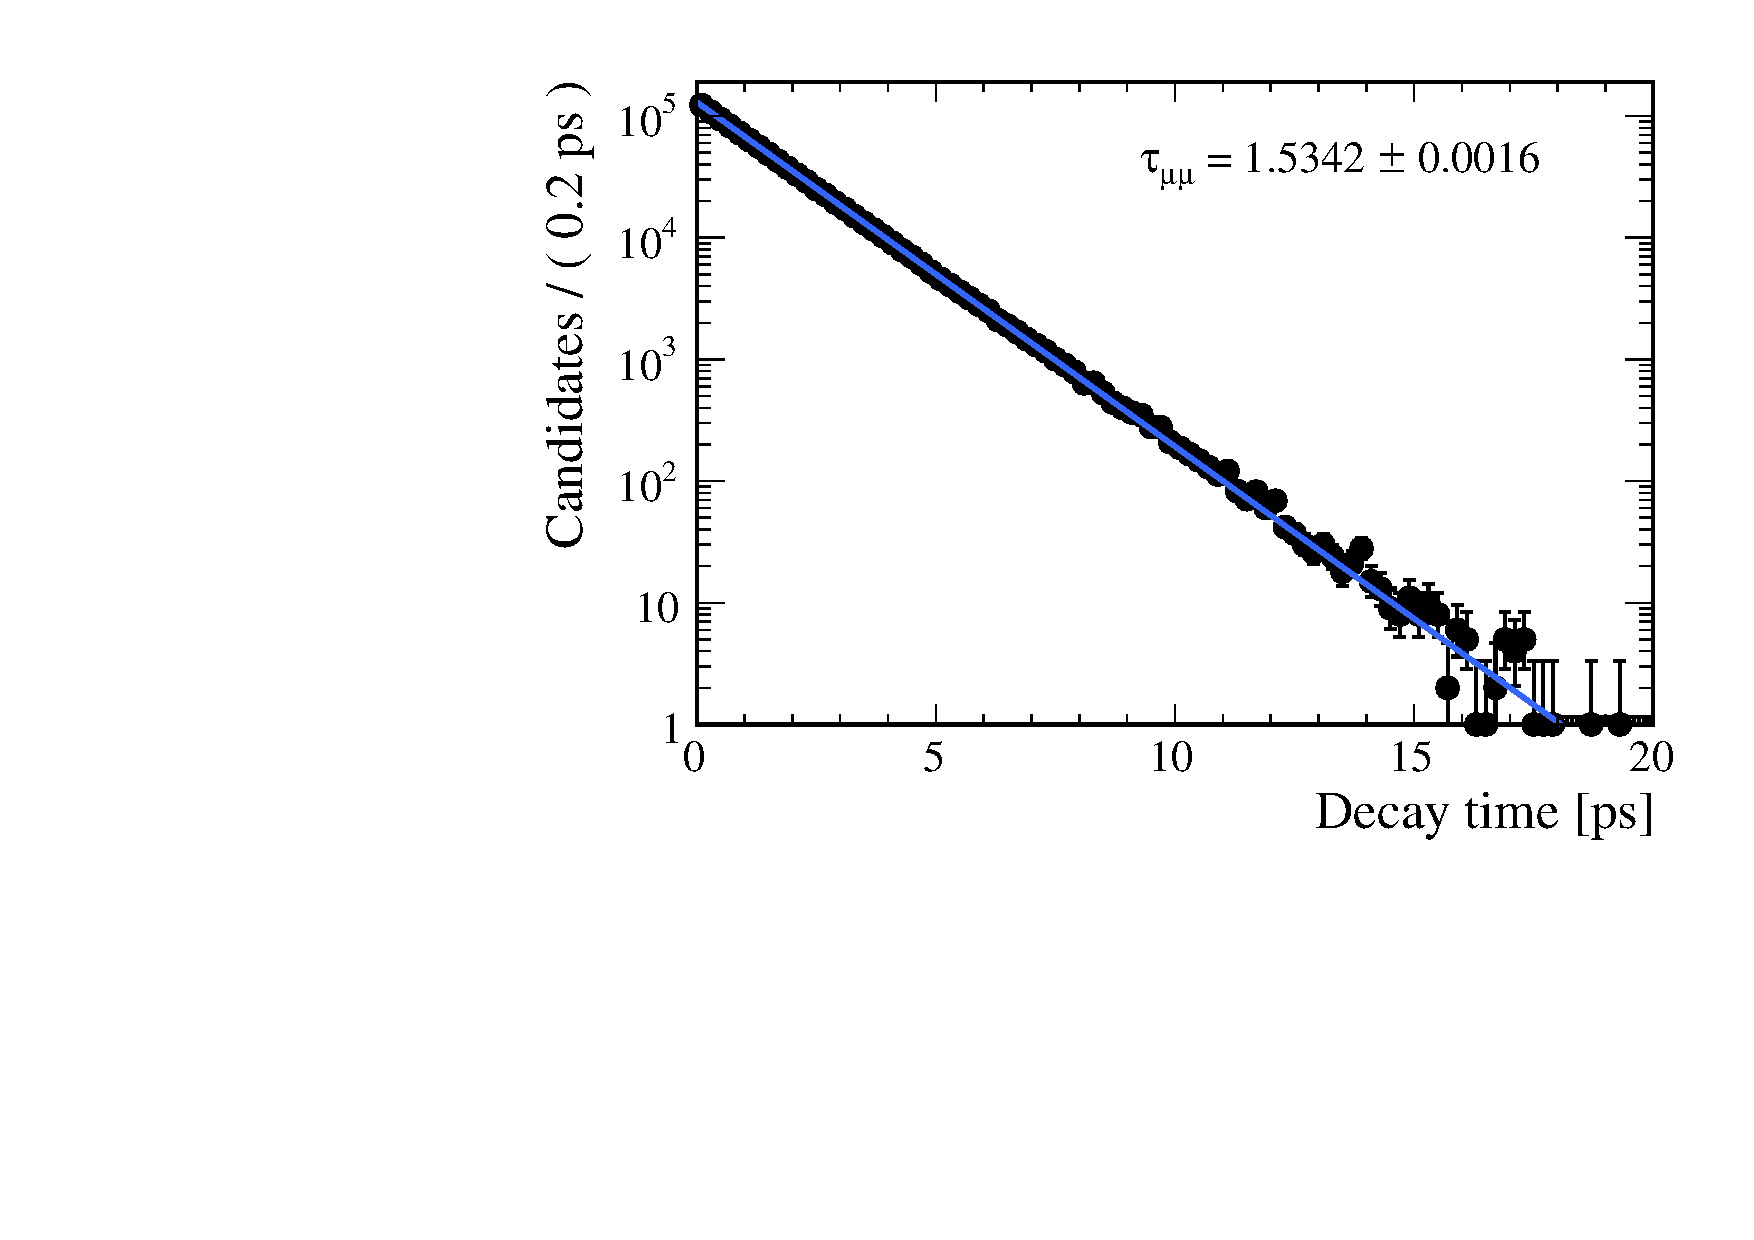
\includegraphics[width=0.49\textwidth]{./Figs/LifetimeSystematics/No_acc_fit.pdf}
    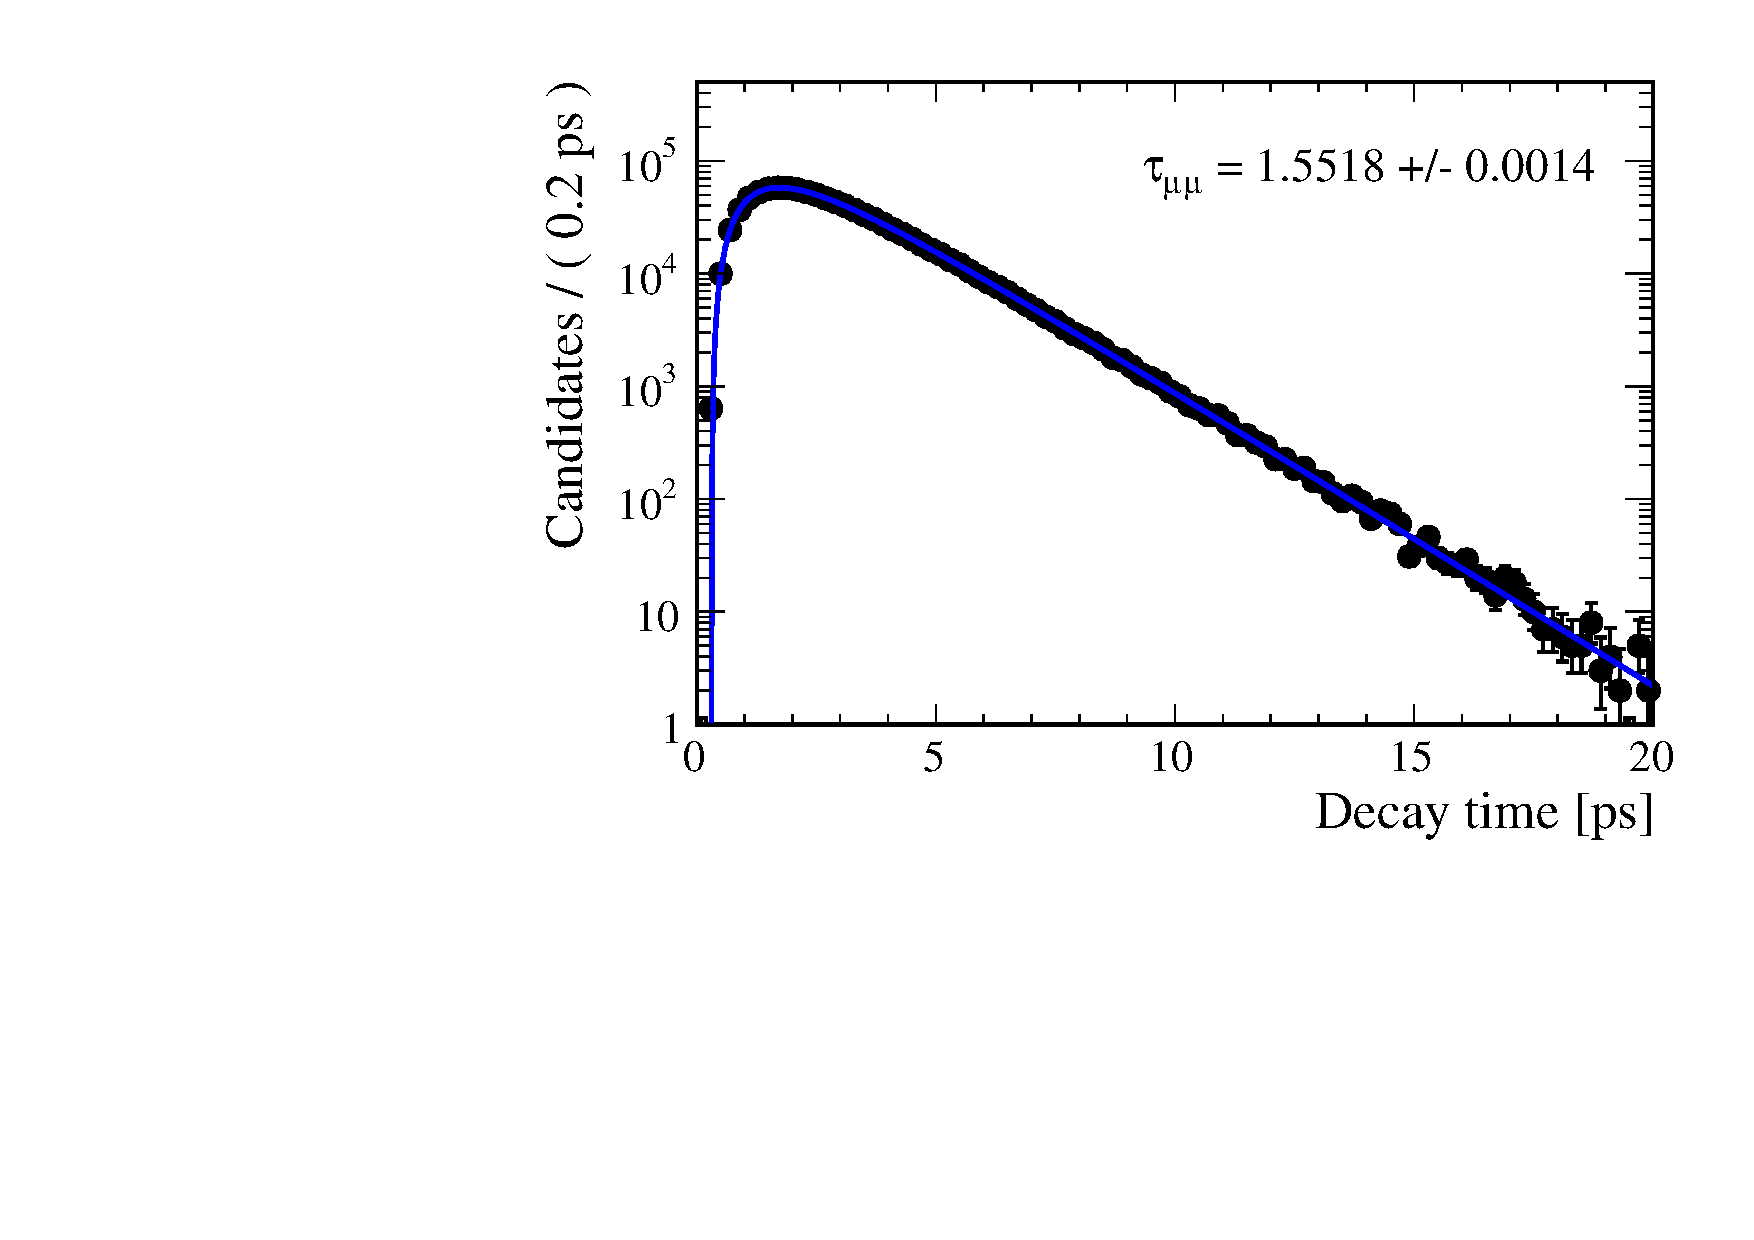
\includegraphics[width=0.49\textwidth]{./Figs/LifetimeSystematics/Acc_fit.pdf}
  \caption{Maximum likelihood fits to the decay time distribution to measure \tmumu for \bsmumu decays that are composed of an equal mix from the heavy and light mass eigenstates. Decay time distributions are generated assuming a flat acceptance function (left) and the acceptance function used to describe \bsmumu decays in data (right).}
  \label{fig:mixofstates}
\end{figure}


\section{Production asymmetry of \bs and $\bar{B_{s}^{0}}$}
\label{sec:productionasymetry}

\section{Summary}
\label{sec:systematicsSummary}

The complete list of systematic uncertainties for \tmumu and \Gmumu are summarised in Table~\ref{}. Adding the uncertainties in quadrature leads to a total uncertainty of X for \tmumu and Y for \Gmumu. The uncertainties correspond to X $\%$ and Y $\%$ of the observed statistical uncertainty for \tmumu and \Gmumu respectively. The small size of the total systematic uncertainties compared to the statistical uncertainties is expected given the observed number of decays. 

Although the systematic uncertainty of \tmumu is larger, it is only a small among larger than the uncertainty on \Gmumu and negligible compared to the statistical uncertainty, therefore is presents no barrier to the result being presented in terms of \tmumu.

%What is the percentage of the unceratines of the measured result? Both statistical and systematic?
